\mychapter{Analytic Functions}\label{ch5}

\section{Conformal invariance}\label{ch5_sec1}

\subsecbkm{ch5_sec1.1}{L\'evy's theorem}
\index{L\'evy's theorem|(}

The connection between two-dimensional Brownian motion and complex analysis comes about through the result of L\'evy that an analytic function composed with a two-dimensional Brownian motion is a time change of another Brownian motion. After describing some notation we will begin with this theorem.

Let $\C$\index{C@$\C$} denote the complex plane, $\D$\index{D@$\D$} the unit disk $\{z : |z| < 1\}$, and $H$ the half-plane $\{z : \Im z > 0\}$. We will let $Z_t$ denote two-dimensional Brownian motion. $Z_t$ can be considered either as $\Re Z_t + \im\Im Z_t$ or as $(\Re Z_t, \Im Z_t)$, depending on the context. We will write just $\tau$ for $\tau_D$ and $\tau_r$ for $\tau_{B(0,r)}$. $\partial_x$ denotes $\partial/\partial x$ and similarly $\partial_y$ denotes $\partial/\partial y$.

We will split L\'evy's theorem into two pieces. First, suppose that $f$ is not constant and that $f$ is entire, that is, analytic on all of $\C$.

\begin{theorem}\label{thm:ch5_1.1}
Let
\begin{equation}\label{eq:ch5_1.1}
A_s = \int_0^s |f'(Z_r)|^2 dr \qquad \text{and} \qquad \sigma_t = \inf\{s : A_s \geq t\}.
\end{equation}
Then $f(Z_{\sigma_t})$ is a two-dimensional Brownian motion.
\end{theorem}

\begin{proof}
If a function is analytic in a domain and its zeroes have a cluster point in the domain, then the function must be identically $0$ (\cite[][p.~127]{Ahlfors1979}). Since $f$ is not identically constant, $f'$ has at most countably many zeroes. Because two-dimensional Brownian motion does not hit a countable set (Proposition \chapref[I]{prop:ch1_5.8}), $A_s$ is strictly increasing. Hence $\sigma_t$ is continuous in $t$, a.s., and $f(Z_{\sigma_t})$ is a continuous process. By Exercise \ref{ex:ch5_1}, $A_s \to \infty$, a.s., as $s \to \infty$.

Suppose $f = u + \im v$. By It\^o's formula,
\begin{equation}\label{eq:ch5_1.2}
    u(Z_t) = u(Z_0) + \int_0^t \nabla u(Z_s) \cdot dZ_s
\end{equation}
and
\begin{equation}\label{eq:ch5_1.3}
    v(Z_t) = v(Z_0) + \int_0^t \nabla v(Z_s) \cdot dZ_s.
\end{equation}
In particular, $u(Z_t)$ and $v(Z_t)$ are martingales. By the Cauchy-Riemann equations we have $|\nabla u(z)|^2 = |\nabla v(z)|^2$ and $\nabla u(z) \cdot \nabla v(z) = 0$ for all $z$. Hence $\lrang{u(Z)}_t = \lrang{v(Z)}_t = A_t$ and $\lrang{u(Z),v(Z)}_t = 0$.

% Note: chnaged Theorem I.5.10 to Corollary I.5.10.

Therefore, $f(Z_{\sigma_t})$ is a continuous two-dimensional process, each of its components is a martingale, $\lrang{u(Z_{\sigma_{\cdot}})}_t = \lrang{v(Z_{\sigma_{\cdot}})}_t = t$, and $\lrang{u(Z_{\sigma_{\cdot}}), (Z_{\sigma_{\cdot}})}_t \allowbreak = 0$. By Corollary \chapref[I]{cor:ch1_5.10}, $f(Z_{\sigma_t})$ is a two-dimensional Brownian motion.
\end{proof}

We next give the version of L\'evy's theorem for functions that are analytic in a domain $D$.

\begin{theorem}\label{thm:ch5_1.2}
Suppose $f$ is analytic in a domain $D$. Let $A_s$ and $\sigma_t$ be as above. If $F_t = f(Z(\sigma_{t \wedge \tau_D}))$, then $F_{t \wedge \tau(f(D))}$ is a two-dimensional Brownian motion stopped on exiting $f(D)$.
\end{theorem}

\begin{proof}
As in the proof of Theorem \ref{thm:ch5_1.1}, $F_t$ is a continuous martingale with $\lrang{\Re F}_t = \lrang{\Im F}_t = t \wedge \tau_D$ and $\lrang{\Re F, \Im F}_t = 0$. Let $W_t$ be a two-dimensional Brownian motion started at $0$ and independent of $Z_t$ and define

\[
    F'_t = \begin{cases}
        F_t, & t \leq \tau_D; \\
        F_{\tau_D} + W_{t-\tau_D}, & t > \tau_D.
    \end{cases}
\]

It is easy to check that $\lrang{\Re F'}_t = \lrang{\Im F'}_t = t$ and $\lrang{\Re F', \Im F'}_t = 0$, and so $F'_t$ is a two-dimensional Brownian motion. It is not hard to see that $f(Z_t)$ first hits $\partial f(D)$ either at the same time or before $Z_t$ first hits $\partial D$. So $F_{t \wedge \tau(f(D))}$ is two-dimensional Brownian motion stopped at the hitting time of $\partial f(D)$.
\end{proof}

\index{L\'evy's theorem|)}

If $f$ is one to one, then in fact the hitting time of $\partial f(D)$ by $f(Z_t)$ is equal to the hitting time of $\partial D$ by $Z_t$.

\subsecbkm{ch5_sec1.2}{Fundamental theorem of algebra}
\index{Fundamental theorem of algebra|(}

For a first application, let us give a probabilistic proof of the fundamental theorem of algebra.

\begin{theorem}\label{thm:ch5_1.3}
Let $P(z)$ be a nonconstant polynomial in $z$. Then there is at least one point $z_0$ such that $P(z_0) = 0$.
\end{theorem}

\begin{proof}
If $P(z) = a_nz^n + a_{n-1}z^{n-1} + \cdots + a_0$ with $a_n \neq 0$, then
\[
    |P(z)| = |a_n||z|^n\Big|1 + \frac{a_{n-1}}{a_n}z^{-1} + \cdots \frac{a_0}{a_n}z^{-n}\Big| \to \infty
\]
as $|z| \to \infty$. Pick $R$ such that $|P(z)| \geq 1$ if $|z| \geq R$.

Suppose $P(z)$ never equals $0$. Since $P(\overline{B(0,R)})$ is compact, hence closed, there is a neighborhood $V$ of $0$ that is disjoint from it. By taking $V$ to have diameter less than $1/2$, $V \cap P(\C) = \emptyset$. However, $P(Z_t)$ is a time change of two-dimensional Brownian motion. Since $P$ is nonconstant, Exercise \ref{ex:ch5_1} says that $\lrang{P(Z)}_t \to \infty$ as $t \to \infty$. That means $P(Z_t)$ hits every neighborhood infinitely often; in particular it hits $V$, a contradiction to $V \cap P(\C) = 0$.
\end{proof}

\index{Fundamental theorem of algebra|)}

\subsecbkm{ch5_sec1.3}{Exit distributions}
\index{Exit distribution|(}

As we saw in Chap.\ \ref{ch2}, if we know the exit distribution of Brownian motion for a domain, we can give an explicit solution to the Dirichlet problem. From L\'evy's theorem, we can compute the exit distribution of two-dimensional Brownian motion in a number of domains. In principle, it can be done for any simply connected region by virtue of the Riemann mapping theorem (see Theorem \ref{thm:ch5_1.14}), but in practice it is not easy except for certain simple domains.

\begin{proposition}\label{prop:ch5_1.4}
Let $W_\alpha$ be the wedge $\{re^{\im\theta} : r > 0, 0 < \theta < \alpha\}$, $0 < \alpha < 2\pi$, and suppose $z_0 \in W_\alpha$. Then
\begin{equation}\label{eq:ch5_1.4}
    \P^{z_0}(Z_{\tau(W_\alpha)} \in (dt,0)) = \alpha^{-1}t^{\pi/\alpha-1}\frac{\Im(z_0^{\pi/\alpha})}{|z_0^{\pi/\alpha} - t^{\pi/\alpha}|^2}dt.
\end{equation}
\end{proposition}

\begin{proof}
The mapping $f(z) = z^{\pi/\alpha}$ maps $W_\alpha$ onto the half-space $H = \{\Im z > 0\}$. Since $0 \notin W_\alpha$, $f$ is analytic on $W_\alpha$. If $C_u = [0,u] \times \{0\}$, then
\[
    \P^{z_0}(Z_{\tau(W_\alpha)} \in C_u) = \P^{f(z_0)}(f(Z_{\tau(W_\alpha)}) \in f(C_u)).
\]
Since $f(Z_t)$ is the time change of a two-dimensional Brownian motion, the place where $f(Z_t)$ exits the domain $H$ and where a two-dimensional Brownian motion exits $H$ are the same. So we need to compute
\mpagebreak
\[
    \P^{z_0^{\pi/\alpha}}(Z'_{\tau_H} \in [0,u^{\pi/\alpha}] \times \{0\}),
\]
where $Z'_t$ is another two-dimensional Brownian motion. By \chapeqref[II]{eq:ch2_1.17}, this is
\[
    \int_0^{u^{\pi/\alpha}} \frac{1}{\pi} \frac{\Im z_0^{\pi/\alpha}}{|w - z_0^{\pi/\alpha}|^2}dw.
\]
Differentiating in $u$ gives (\ref{eq:ch5_1.4}).
\end{proof}

The mapping $f(z) = \exp(z)$ maps the strip $S = \{0 < \Im z < \pi/2\}$ onto the half-plane $H$. The same method of proof gives the exit distribution of a strip (Exercise \ref{ex:ch5_3}).

Sometimes a combination of conformal mapping and other techniques is useful. For example, to find the exit distribution of $W_\alpha \cap B(0,M)$ or $\{0 < \Im z < \pi/2, \Re z < M\}$, conformal mapping reduces the problem to finding the exit distribution of $H \cap B(0,N)$ for suitable $N$. This is easily done by the reflection principle. For later, we only need the following bound.

\begin{proposition}\label{prop:ch5_1.5}
There exists $c$ independent of $N$ such that if $z_0$ is in $H \cap B(0,N/2)$, then
\[
    \P^{z_0}(Z_{\tau(H \cap B(0,N))} \in \partial B(0,N)) \leq c|z_0|/N.
\]
\end{proposition}

\begin{proof}
\[
    h_1(z) = \P^z(Z_{\tau(B(0,N))} \in H \cap \partial B(0,N))
\]
is harmonic in $B(0,N)$. If $z = x + \im y$ and $h_2(z) = h_1(x-\im y)$, then by symmetry considerations and the fact that $\overline{Z_t}$, the complex conjugate of $Z_t$, is another Brownian motion,
\[
    h_2(z) = \P^{x+\im y}(\overline{Z}_{\tau(B(0,N))} \in H^c \cap \partial B(0,N))
\]
is harmonic in $B(0,N)$. (This is the reflection principle in disguise.) The difference $h = h_1 - h_2$ is harmonic in $B(0,N)$, takes boundary value $1$ on $H \cap \partial B(0,N)$ and takes the value $0$ on $\partial H \cap B(0,N)$. Therefore $h(z) = \P^z(Z_{\tau(H \cap B(0,N))} \in \partial B(0,N))$ for $z \in H \cap B(0,N)$. By Corollary \chapref[II]{cor:ch2_1.4}, $|\nabla h|$ is bounded by $c/N$ in $H \cap B(0,N/2)$. Since $h(0) = 0$, the proposition follows.
\end{proof}

\index{Exit distribution|)}

\subsecbkm{ch5_sec1.4}{Maximum modulus principle}
\index{Maximum modulus principle|(}

If $u$ is harmonic in $D$ and continuous on $\overline{D}$, and $D$ is a bounded domain, then $\sup_{\overline{D}} u = \sup_{\partial D} u$. The same is true for analytic functions. Recall from the remarks following Definition \chapref[II]{def:ch2_6.6} that $f$ is subharmonic if $-f$ is superharmonic.

\begin{proposition}[Maximum modulus principle]\label{prop:ch5_1.6}
If $D$ is a bounded domain and $f$ is analytic in $D$ and continuous in $\overline{D}$, then $\sup_{\overline{D}} |f| = \sup_{\partial D} |f|$.
\end{proposition}

\begin{proof}
If $f = u + \im v$ where $u$ and $v$ are harmonic, then $|f|^2 = u^2 + v^2$ is subharmonic, since $\Delta(u^2) = 2|\nabla u|^2 \geq 0$ and the same for $\Delta(v^2)$. So $|f(z)|^2 \leq \E^z|f(Z_{\tau_D})|^2 \leq \sup_{\partial D} |f|^2$ for $z \in D$. Taking square roots gives our result.
\end{proof}

% Note: changed "...theorem say" in the following paragraph

If $D$ is not bounded, this need not be true at all. For example, let $D = H$ and $f(z) = e^{-\im z} = e^{-\im x+y}$. This is bounded on $\partial H$, but not on $H$. The Phragm\'en-Lindel\"of theorem\index{Phragm\'en-Lindel\"of theorem|(} says that if $f$ also satisfies a growth condition, the maximum modulus result still holds.

First we need a lemma. Although one has to be careful when defining $\log f(z)$ so as to avoid the zeroes of $f$, $|f(z)|$ is a nonnegative real number and there is no problem defining $\log^+ |f(z)|$, where $\log^+ x = 0 \vee \log x$.

\index{Maximum modulus principle|)}

\begin{lemma}\label{lem:ch5_1.7}
If $f$ is analytic in $D$, then $\log^+ |f(z)|$ is subharmonic and continuous in $D$.
\end{lemma}

\begin{proof}
If $|f(z_0)| \leq 1/2$ for some $z_0 \in D$, then by the continuity of $f$, $|f(z)| < 1$ in a neighborhood of $z_0$ and so $\log^+ |f(z)| = 0$ in a neighborhood of $z_0$. If $|f(z_0)| > 1/2$ for some $z_0 \in D$, the same will be true for $z$ in a neighborhood of $z_0$. A direct calculation shows that $\log |f(z)|$ is harmonic in this neighborhood (cf.\ Sect.\ \chapref[II]{ch2_sec3}), and so $\log^+ |f(z)|$ is subharmonic and continuous. Therefore $\log^+ |f(z)|$ is subharmonic and continuous in a neighborhood of every point in $D$.
\end{proof}

\begin{theorem}\label{thm:ch5_1.8}
Suppose $f$ is analytic in $H$, continuous on $\overline{H}$, and bounded by $K$ on $\partial H$. If for some $\alpha < 1$,
\[
    |f(z)| \leq c\exp(|z|^\alpha),
\]
then $|f(z)| \leq K$ for all $z \in H$.
\end{theorem}

\begin{proof}
By multiplying $f$ by a constant, we may suppose that $K \geq 1$. Fix $z_0 \in H$. Let $\epsilon > 0$. Let $u(z) = \log^+ |f(z)|$. By our growth assumption on $f$, there exists $M > 2|z_0|$ large such that $u(z) \leq \epsilon|z|$ if $|z| \geq M$. Then by Proposition \ref{prop:ch5_1.5}
\begin{align*}
    u(z_0) &\leq \E^{z_0} u(Z_{\tau(B(0,M)\cap H)}) \\
    &\leq (\log K)\P^{z_0}(Z_{\tau(B(0,M)\cap H)} \in \partial H) \\
    &\qquad+ \epsilon M\P^{z_0}(Z_{\tau(B(0,M)\cap H)} \in \partial B(0,M) \cap H) \\
    &\leq \log K + c\epsilon.
\end{align*}
    Since $\epsilon$ is arbitrary, $u(z_0) \leq \log K$.
\end{proof}

As a corollary, if $S$ is the strip $\{0 < \Im z < \pi/2\}$, we have

\begin{corollary}\label{cor:ch5_1.9}
Suppose $f$ is analytic in a strip $S$ and continuous on $\overline{S}$. Sup\-pose $|f|$ is bounded by $K$ on $\partial S$. If for some $\alpha < 1$, $|f(z)| \leq c\exp(|\exp(\alpha z)|)$ for all $z \in S$, then $|f|$ is bounded by $K$ in $S$.
\end{corollary}

\begin{proof}
Let $F(z) = \log z$. Then $|f(F(z))|$ is bounded by $K$ on $H$ and $|f(F(z))| \leq c\exp(|z|^\alpha)$. By Theorem \ref{thm:ch5_1.8}, $|f(F(z))| \leq K$ on $\partial H$, which implies $|f|$ is bounded by $K$ in $S$.
\end{proof}

\index{Phragm\'en-Lindel\"of theorem|)}

% Note: changed Theorem 1.9 to Corollary 1.9 in the next paragraoh

One application of the Phragm\'en-Lindel\"of result is to the interpolation of linear operators. We use Corollary \ref{cor:ch5_1.9} to prove the ``three lines lemma,''\index{Three lines lemma} which could also be derived as a consequence of the maximum modulus principle.

\begin{lemma}\label{lem:ch5_1.10}
Suppose $\varphi$ is bounded on the strip $\{0 \leq \Re z \leq 1\}$ and analytic in the interior. If $|\varphi| \leq M_0$ on $\{\Re z = 0\}$, $|\varphi| \leq M_1$ on $\{\Re z = 1\}$, and $t \in (0,1)$, then $|\varphi| \leq M_0^{1-t}M_1^t$ on $\{\Re z = t\}$.
\end{lemma}

\begin{proof}
Let $\psi(z) = \varphi(z)M_0^{z-1}M_1^{-z}$. Since $M_0^z = e^{z\log M_0}$, then  $|M_0^z| = e^{\Re(z\log M_0)}\le c$ on the strip. Similarly $M_1^{-z}$ is bounded on the strip, hence $\psi$ is bounded and continuous on the strip and analytic in the interior. When $\Re z = 0$, $|\psi(z)|\le 1$ and the same is true when $\Re z = 1$. By a rotation, scaling, and Corollary \ref{cor:ch5_1.9}, $|\psi|$ is bounded by $1$ on the strip. Therefore $|\varphi(z)| \leq |M_0^{1-z}||M_1^z| = M_0^{1-t}M_1^t$ if $\Re z = t$.
\end{proof}

This leads to the Riesz-Thorin interpolation theorem\index{Riesz-Thorin interpolation theorem|(}.

\begin{theorem}\label{thm:ch5_1.11}
Suppose $T$ is a bounded linear functional on $L^p$ and on $L^q$. Suppose $1 \leq p < r < q \leq \infty$. Then $T$ is a bounded linear functional on $L^r$ and $\|T\|_r \leq \|T\|_p^{1-t}\|T\|_q^t$ if $1/r = (1-t)/p + t/q$.
\end{theorem}

\begin{proof}
Let $M_0 = \|T\|_p$, $M_1 = \|T\|_q$. The key step is to show
\begin{equation}\label{eq:ch5_1.5}
    \int (Tf)g \leq M_0^{1-t}M_1^t
\end{equation}
if $f \in L^r$ with $\|f\|_r = 1$ and $g \in L^{r'}$ with $\|g\|_{r'} = 1$, where $r'$ is the conjugate exponent to $r$ (that is, $1/r + 1/r' = 1$), and $f$ and $g$ are simple functions. For then, if \eqref{eq:ch5_1.5} holds, taking the supremum over such simple functions $g$ implies that $\|Tf\|_r \leq M_0^{1-t}M_1^t$.

To prove \eqref{eq:ch5_1.5}, let us write $f = \sum_{j=1}^n a_j1_{A_j}$ and $g = \sum_{k=1}^m b_k1_{B_k}$, where the $A_j$s are disjoint and so are the $B_k$s. If $a_j = |a_j|e^{\im\alpha_j}$ and $b_k = |b_k|e^{\im\beta_k}$, let
\[
    f_z = \sum |a_j|^{s(z)/s(t)}e^{\im\alpha_j}1_{A_j}
\]
and
\[
    g_z = \sum |b_k|^{(1-s(z))/(1-s(t))}e^{\im\beta_k}1_{B_k},
\]
where
\mpagebreak
\[
    s(z) = \frac{1-z}{p} + \frac{z}{q}
\]
and $s(t)$ denotes $s(t + 0\im)$. Let
\begin{align*}
    \varphi(z) &= \int (Tf_z)g_z \\
    &=\sum_{j,k}|a_j|^{s(z)/s(t)}|b_k|^{(1-s(z))/(1-s(t))}e^{\im (\alpha_j+\beta_k)}\int (T1_{A_j})1_{B_k}.
\end{align*}

$\varphi$ is an entire function of $z$. Note $\varphi(t) = \int (Tf)g$. Also, the exponents of $|a_j|$ and $|b_k|$ have bounded real parts, hence $\varphi$ is bounded on the strip $\{0\le \Re z \le 1\}$.

If we write $z=x+\im y$, then when $\Re z = 0$,
\[
    s(z)=\frac{1-\im y}{p}+\frac{\im y}{q}=\frac{1}{p}+\im y\Big(\frac{1}{q}-\frac{1}{p}\Big)
\]
and so $f_{\im y}=|f|^{(1/p)/s(t)}=|f|^{r/p}$. Therefore
\[
    \|f_{\im y}\|_p^p = \Big(\int |f_{\im y}|^p\Big)^{1/p} = \Big(\int  |f|^r\Big)^{1/p} = 1
\]
by our normalization. Similarly, if $p'$ is the conjugate exponent to $p$, $\|g_{\im y}\|_{p'}=1$, By H\"older's inequality,
\[
    |\varphi(\im y)|=\|T f_{\im y}\|_p\|g_{\im y}\|_{p'}\leq M_0\|f_{\im y}\|_p\|g_{\im y}\|_{p'}\leq M_0.
\]
So $\varphi$ is bounded by $M_0$ on $\{\Re z = 0\}$. Similarly, it is bounded by $M_1$ on $\{\Re z = 1\}$. By Lemma \ref{lem:ch5_1.10}, $\varphi(z)$ is bounded on $\{\Re z = t\}$ by $M_0^{1-t}M_1^t$.
\end{proof}

\index{Riesz-Thorin interpolation theorem|)}

The Marckinkiewicz interpolation theorem\index{Marcinkiewicz interpolation theorem} (Theorem \chapref[IV]{thm:ch4_7.21}) says that if $T$ is sublinear, i.e., $|T(f + g)| \leq |T(f)| + |T(g)|$ and $|T(cf)| = |c||T(f)|$, and $T$ is weak type $(p,p)$ and weak type $(q,q)$, then $T$ is strong type $(r,r)$. Weak type $(p,p)$ means that $|\{x : |Tf(x)| > \lambda\}| \leq c\|f\|_p^p/\lambda^p$ for all $\lambda > 0$, while strong type $(r,r)$ simply means that $T$ is a bounded linear functional on $L^r$. By Chebyshev's inequality, if an operator is strong type $(p,p)$, it is also weak type $(p,p)$. Note the Marckinkiewicz interpolation theorem has weaker assumptions than the Riesz-Thorin theorem. However the bound on $\|T\|_r$ from the Riesz-Thorin theorem is much better.

Both interpolation theorems can be modified to handle the case where $T : L^{p_1} \to L^{p_2}$ and $T : L^{q_1} \to L^{q_2}$ to conclude $T : L^{r_1} \to L^{r_2}$ if $p_1,p_2,q_1,q_2,r_1$, and $r_2$ are chosen appropriately. Both theorems have been extended to quite abstract settings, and the Riesz-Thorin theorem and the Marckinkiewicz theorem are the basis for the complex and real methods of interpolation, respectively; see \cite{BerghLofstrom1976}.

\subsecbkm{ch5_sec1.5}{Riemann mapping theorem}

We now use some ideas from Chap.\ \ref{ch2} to give a proof of the Riemann mapping theorem, which says that any simply connected domain other than the whole plane can be mapped one to one onto the unit disk. One nice feature of the construction we give here is that it is somewhat constructive.

First we recall the argument principle\index{Argument principle}: if $\gamma$ is a simple closed curve enclosing a domain $D$, $f$ is analytic in a domain $D'$ containing $\overline{D}$, and $f$ has no zeroes on $\gamma$, then
\[
    \frac{1}{2\pi \im}\int_\gamma \frac{f'(z)}{f(z)}dz
    % Note: replaced i with \im
\]
is equal to the number of zeroes of $f$ in $D$, counted according to their multiplicity (\cite[see][p.~151]{Ahlfors1979}).

We will need the following corollary.

\begin{corollary}[Rouch\'e's theorem\index{Rouch\'e's theorem}]\label{cor:ch5_1.12}
Let $\gamma$ and $D$ be as above. Suppose $f$ and $g$ are analytic in a domain $D'$ containing $\overline{D}$ and $|f(z) - g(z)| < |f(z)|$ on $\gamma$. Then $f$ and $g$ have the same number of zeroes in $D$.
\end{corollary}

\begin{proof}
Let $F(z) = g(z)/f(z)$. The hypothesis implies that $|F(z) - 1| < 1$. By the maximum modulus principle applied to $F - 1$, $|F - 1| < 1$ on $D$, and so $F$ has no zeroes in $D$. Therefore $F'/F$ is analytic in $D$. Applying Cauchy's integral theorem and the argument principle, we see $F$ has no zeroes in $D$. Since $F$ is analytic in $D$, that implies that $f$ and $g$ must have zeroes at the same places with the same multiplicity.
\end{proof}

\index{Green function!Two-dimensional Brownian motion|(}

Since most of the results in Sect.\ \chapref[II]{ch2_sec3} were for $d$-dimensional Brownian motion with $d \geq 3$, we take a few moments to present some facts about Green functions for two-dimensional Brownian motion. For simplicity, we will only consider domains $D$ such that every point of $\partial D$ is regular for $D^c$ and such that $D$ is contained in some half-plane (see \cite{PortStone1978} for the full story). By a change of coordinate systems, we may suppose $D \subseteq H$.

Let
\begin{equation}\label{eq:ch5_1.6}
    u_H(x,y) = -\pi^{-1}\log|x-y| + \pi^{-1}\log|\overline{x}-y|, \qquad x,y \in H.
\end{equation}
Since $|\overline{x}-y| = |x-\overline{y}|$, $u_H$ is symmetric in $x$ and $y$. If we let $\widehat{Z}_t$ be two-dimensional Brownian motion killed on exiting $H$, then by Exercise \chapref[II.8]{ex:ch2_44},
\[
    \E^x\int_0^\infty f(\widehat{Z}_t)dt = \int_H u_H(x,y)f(y)dy
\]
if $f$ is nonnegative and measurable. Set
\begin{equation}\label{eq:ch5_1.7}
    g_D(x,y) = u_H(x,y) - \E^xu_H(\widehat{Z}_{\tau_D},y), \qquad x,y \in D,
\end{equation}
and $g_D(x,y) = 0$ if $x$ or $y$ is in $D^c$. We call $g_D$ the Green function for $D$.

\begin{proposition}\label{prop:ch5_1.13}
Suppose $D \subseteq H$ and every point of $\partial D$ is regular for $D^c$.
\begin{enumerate}
    \item If $f \geq 0$, then $\int g_D(x,y)f(y)dy = \E^x\int_0^{\tau_D} f(\widehat{Z}_t)dt$.
    \item $g_D(x,y)$ differs from $-\pi^{-1}\log|x-y|$ by a function that is harmonic in $D$.
    \item $g_D(x,y)$ is symmetric in $x$ and $y$.
\end{enumerate}
\end{proposition}

\begin{proof}
(a) follows by the argument used in equations \chapeqref[II]{eq:ch2_3.14} through \chapeqref[II]{eq:ch2_3.16} with $u$ replaced by $u_H$. For each $y$, $\E^xu_H(\widehat{Z}_{\tau_D},y)$ is harmonic in $x$ on the set $D$. Hence $g_D$ differs from $u_H$ by a function that is harmonic in $D$. (b) follows, since $-\pi^{-1}\log|x-\overline{y}|$ is harmonic in $x$ on the set $H$. To prove (c), note that the transition density of $\widehat{Z}_t$ is symmetric in $x$ and $y$ by Exercise \chapref[II.8]{ex:ch2_43}. So just as in the proof of Proposition \chapref[II]{prop:ch2_4.1},
\[
    \int_C \P^x(\widehat{Z}_t \in A, \tau_D \geq t)dx = \int_A \P^x(\widehat{Z}_t \in C, \tau_D \geq t)dx.
\]
If we integrate this over $t$ from $0$ to $\infty$, on the left we obtain
\[
    \int_C \E^x\int_0^{\tau_D} 1_A(\widehat{Z}_t)dt\, dx = \int_C\int_A g_D(x,y)dy\, dx.
\]
Similarly, on the right we have $\int_A\int_C g_D(x,y)dy\, dx$, from which we con\-clude that $g_D(x,y) = g_D(y,x)$ for almost every pair $(x,y)$. Also, $g_D(x,y)$ is continuous in $x$ on the set $D-\{y\}$ since it is harmonic there, and it is continuous in $y$ on the set $D-\{x\}$ by the continuity of $u_H$ in $y$. (c) follows.
\end{proof}

\index{Green function!Two-dimensional Brownian motion|)}

We now prove the Riemann mapping theorem\index{Riemann mapping theorem|(}. Recall that a domain $D$ is simply connected\index{Simply connected domain} if $D^c$ consists of a single unbounded component.

\begin{theorem}\label{thm:ch5_1.14}
If $D$ is a simply connected domain other than the entire plane and $z_0 \in D$, then there exists $f$ analytic in $D$ mapping $D$ one to one onto the unit disk with $f(z_0) = 0$ and $f'(z_0) > 0$.
\end{theorem}

It is not hard to show that $f$ must be unique; \cite[see][p.~222]{Ahlfors1979}.

\tweakpage{0.5}

\begin{proof}
We first show that we may take $D$ to be bounded. Suppose $D$ is unbounded. If $D$ is not the entire complex plane, there is at least one point not in $D$. Let us suppose that point is $0$. Since $D$ is simply connected, we can define a single-valued branch of $\log z$, namely, we connect a fixed point $z_0$ in $D$ to $z$ by a curve $\gamma$ and let $\log z = \int_\gamma dz/z + \log|z_0|$. We can define $f_1(z) = z^{1/2} = e^{(1/2)\log z}$ as a single-valued analytic function in $D$. $f_1$ is one to one, since it has an inverse, namely, $z^2$. Let $D' = f_1(D)$.

There exists a point $z_1$ and a neighborhood $U$ of $z_1$ contained in $D'$. We claim $-U$ is disjoint from $D'$. For if $z \in -U$ and $z \in D'$, then $z^2$ and $(-z)^2$ would both be in $D$, contradicting the fact that $f_1$ is one to one. Therefore the complement of $D'$ contains some ball, say $B(z_2,\epsilon)$. Let $f_2$ be inversion in the ball $B(z_2,\epsilon)$; we set $f_2(z) = \epsilon^2/(z-z_2)$. $f_2$ is clearly one to one and analytic and now $D'' = f_2(D') \subseteq B(z_2,\epsilon)$. We have thus reduced the problem to the case of $D$ bounded.

% Note: replaced i with \im in the following paragraph

Now suppose $D$ is bounded. We proceed to define $f$. By Proposition \chapref[II]{prop:ch2_1.14}, every point of $\partial D$ is regular for $D^c$. Let $g(z) = g_D(z_0,z)$ be the Green function for $D$. Then $g(z) = 0$ if $z \in \partial D$. What we would like to do is to let $\widetilde{g}$ be the conjugate harmonic function to $g$ on $D-\{z_0\}$. Then we would let $f(z) = \exp(-\pi[g(z) + \im\widetilde{g}(z)])$. Since $g(z) \geq 0$, then $|f(z)| \leq 1$ and $f$ maps $D$ into the unit disk. The difficulty is that $g$ is harmonic in $D-\{z_0\}$, not in $D$, and $D-\{z_0\}$ is not simply connected. So a single-valued conjugate harmonic function need not exist in $D-\{z_0\}$ (e.g., $\log|z|$ is harmonic in $\D-\{0\}$ without a single-valued conjugate harmonic function in that domain).

What we do is fix $z_1 \in D-\{z_0\}$ and if $z \in D$, we connect $z_1$ to $z$ by a curve $\psi$ lying in $D-\{z_0\}$. Then let
\begin{equation}\label{eq:ch5_1.8}
    \widetilde{g}(z) = \int_\psi (-\partial_y g + \im\partial_x g)dz, \qquad f(z) = \exp(-\pi[g(z) + \im\widetilde{g}(z)]).
\end{equation}
Although $\widetilde{g}$ is not uniquely defined, $f$ is nevertheless single valued (see Exercise \ref{ex:ch5_4}).

We show $f$ is analytic in $D$. $f$ is clearly analytic if $z \neq z_0$. By Proposition \ref{prop:ch5_1.13}, $|g(z) - (-\pi^{-1}\log|z-z_0|)|$ remains bounded in a neighborhood of $z_0$. Therefore $f$ is bounded in a neighborhood of $z_0$. It follows that $z_0$ is a removable singularity for $f$. Since $\lim_{z \to z_0} f(z) = 0$ by \eqref{eq:ch5_1.8}, $f(z_0) = 0$ as we wished. Since $g(z) \to \infty$ only if $z \to z_0$, in fact $z_0$ is the only zero of $f$.

Note $g(z) = -\pi^{-1}\log|z-z_0|$ plus a harmonic function, say $u$. Since $f$ has a zero at $z_0$, it follows that $f(z)=(z-z_0)h(z)$, where $h$ is analytic and $|h(z)|=e^{-\pi u(z)}$. Since $u$ is harmonic at $z_0$, it is differentiable there, which implies $f'(z_0) \neq 0$. So the zero at $z_0$ is a simple one. If we follow $f$ by the application of the appropriate linear fractional transformation, we can arrange $f'(z_0)$ to be real and positive.

\tweakpage{0.5}

Let us show $f$ is one to one. Suppose $f(z_1) = w$. Then $g(z_1) = -\pi^{-1}\log|w|$. Since $g(z) \to \infty$ as $z \to z_0$ and $g(z) \to 0$ as $z$ tends to the boundary, $\{z : g(z) = w\}$ is a positive distance from $\partial D$ and from $z_0$. For each $z \in D-\{z_0\}$, there is a neighborhood of $z$ in which $\widetilde{g}$, the conjugate harmonic function to $g$, is single-valued. $g+\im\widetilde{g}$ is analytic in this neighborhood, hence the derivative is analytic. Since $g$ cannot be constant in a subdomain (Exercise \chapref[III.6]{ex:ch3_25}), $\nabla g$ is zero for only countably many points inside this neighborhood. Therefore there are only countably many points in $D-\{z_0\}$ at which $\nabla g$ is zero. Let $\epsilon > 0$ be small and let $\gamma$ be the set $\{z : g(z) = -\pi^{-1}\log|w|-\epsilon\}$. We can choose $\epsilon$ so that $\gamma$ contains no zero of $\nabla g$. By the implicit function theorem, $\gamma$ is a smooth curve. We claim $\gamma$ is a simple closed curve. It is closed, because if not, we could find a curve $\psi$ connecting $z_0$ to $\partial D$ avoiding $\gamma$; this is impossible because $g(z_0) = \infty$, $g = 0$ on $\partial D$, and $g$ is continuous in $D-\{z_0\}$. Suppose $\gamma$ were not simple. Then there is a piece of $\gamma$ that encloses a subdomain $D'$, with $z_0 \notin D'$. Since $g$ is constant on $\gamma$, hence on $\partial D'$, then by the maximum principle, $g$ is constant in $D'$. Then $\nabla g=0$ in $D'$, contradicting what we had earlier.

Let us now apply Rouch\'e's theorem to the curve $\gamma$ and the functions $f$ and $f-w$. On $\gamma$,
\[
    |f-(f-w)| = |w|.
\]
On $\gamma$, $|f(z)| = e^{-\pi g(z)} = e^{\pi\epsilon}|w| > |w|$. So by Rouch\'e's theorem, $f$ and $f-w$ have the same number of zeroes inside $\gamma$. Since $f$ is zero only at $z_0$, this says $f-w$ has only one zero.

That $f$ is onto the unit disk comes from the same proof. Pick $w$ in the unit disk and define $\gamma$ as above. Since $f-w$ has exactly one zero in $D$, there must exist a point $z_1$ such that $f(z_1) = w$.
\end{proof}

\index{Riemann mapping theorem|)}

It is not necessarily true that $f$ can be extended continuously to $\overline{D}$ (suppose $D$ is the slit disk). However if $\partial D$ is a simple closed curve, then $f$ can be extended continuously to $\overline{D}$ (\cite{Pommerenke1975}). If $\partial D$ is even smoother, one can ask about further smoothness of $f$, for example, does $f'$ exist? See Sect.\ \ref{ch5_sec5}.

\section{Range of analytic functions}\label{ch5_sec2}

In this section we give probabilistic proofs of Picard's little theorem and the Koebe distortion theorem. The first says that the range of an entire function is either all of $\C$ or else $\C$ minus at most one point. The second says that the range of a one to one analytic function on $\D$ contains a ball of a certain size.

\subsecbkm{ch5_sec2.1}{Picard's theorem}

Picard's little theorem\index{Picard's theorem|(} says the following.

\begin{theorem}\label{thm:ch5_2.1}
If $f$ is an entire function and nonconstant, then the range of $f$ consists of $\C$ minus at most one point.
\end{theorem}

The analytic proof of this fact takes some doing. We give an elegant proof due to \cite{Davis1975}.

Recall that two closed curves $\gamma_1$ and $\gamma_2$ are homotopic\index{Homotopic|(} in a domain $D$ if $\gamma_1$ can be stretched continuously to $\gamma_2$. More precisely, suppose $\gamma_1$ and $\gamma_2$ are continuous mappings of $[0,1]$ into a domain $D$ with $\gamma_i(0) = \gamma_i(1)$, $i = 1,2$. $\gamma_1$ and $\gamma_2$ are homotopic if there exists $F$ mapping $[0,1]^2$ into $D$ such that $F$ is continuous, $F(s,0) = \gamma_1(s)$ for all $s \in [0,1]$, $F(s,1) = \gamma_2(s)$ for all $s \in [0,1]$, and $F(0,t) = F(1,t)$ for all $t \in [0,1]$. The set of curves homotopic to each other is easily seen to be an equivalence class. Also, if $\gamma_1$ and $\gamma_2$ are homotopic to each other and $f$ is continuous, then $f(\gamma_1)$ and $f(\gamma_2)$ are homotopic to each other. In a simply connected domain each closed curve is homotopic to the curve $\gamma_0$ that is a single point in the domain.

\begin{proof}[Proof of Theorem \ref{thm:ch5_2.1}]
If $f(\C)$ omits more than one point of $\C$, we can assume without loss of generality that two of the points it omits are $-a$ and $b$, where $a$ and $b$ are positive reals, and that $f(0) = 0$. Since $f$ is entire, $|f'| > 0$ except for a countable set, and by the recurrence of Brownian motion, $\int_0^t |f'(Z_s)|^2ds \to \infty$ as $t \to \infty$ (cf.\ Exercise \ref{ex:ch5_1}). Hence $f(Z_t)$ is the time change of a Brownian motion (not killed or stopped).

Let $\epsilon$ be small so that if $|z| < \epsilon$, $f(z)$ can be connected to $0$ by a curve lying in $f(\C) \cap B(0,(a \wedge b)/2)$. Infinitely often $Z_t \in B(0,\epsilon)$. Let $L_t$ be the straight line segment connecting $Z_t$ to $0$. The curve consisting of adding the line segment $L_t$ to the end of $Z_t$ is a closed curve homotopic to the single point $0$. So the curve consisting of adding $f(L_t)$ to the end of $f(Z_t)$ must also be homotopic to a single point. By Proposition \ref{prop:ch5_2.2}, for $t$ sufficiently large, this curve is not homotopic to a single point, a contradiction.
\end{proof}

\begin{proposition}\label{prop:ch5_2.2}
Let $L_t$ be as in the proof above. With probability one, there exists $t_0$ (depending on $\omega$) such that if $t > t_0$, the curve formed by adding $f(L_t)$ to the end of $f(Z_t)$ is not homotopic to a single point.
\end{proposition}

\index{Homotopic|)}

\textbf{Warning:} Although this proof is obviously modeled after the account in \cite{Durrett1984}, there are significant differences. For example, the definition of reduced sequences is different.

\begin{proof}
Let
{\setlength{\abovedisplayskip}{0em}
\begin{align*}
    A_0 &= \{-a < x < b, y = 0\}, \\
    A_1 &= \{x < -a, y = 0\}, \\
    A_2 &= \{x > b, y = 0\}, \\
    A_3 &= \{x = -a~\text{or}~x = b, y > 0\}, \\
    A_4 &= \{x = -a~\text{or}~x = b, y < 0\}.
\end{align*}
}

Let $T_1 = 0$. Let $b_i \in \{0,1,2,3,4\}$ be such that $f(Z_{T_i}) \in A_{b_i}$, and
\[
    T_{i+1} = \inf\{t > T_i : f(Z_t) \in \cup_{j=0}^4 A_j - A_{b_i}\}.
\]

Thus the $T_i$s are the times to hit one of the sets $A_j$ different from the last one hit.

\tweakpage{0.5}

We form the sequence $0b_1b_2\ldots b_n$, and then form the reduced sequence\index{Reduced sequence|(} as follows:
\begin{enumerate}
    \item If our sequence ends in $030$ or $040$, delete the last two entries.
    \item If the last entry is the same as the second from the last and the next to the last entry is not $0$, delete the last two entries. (So $\ldots 0424$ becomes $\ldots 04$, but $\ldots 3404$ does not become $\ldots 34$.)
    \mpagebreak
    \item If the sequence ends in a $0$ and has the form $\ldots 0b_{i_1}\ldots b_{i_j}0b_{i_j}\ldots b_{i_1}0$ (i.e., the piece between the next to the last $0$ and the end is the same as the piece from the second from the last $0$ and the next to the last $0$ in reverse order), eliminate everything after the second to the last 0$0$. For example, $\ldots 04231401324$ becomes $\ldots 0$.
\end{enumerate}

We apply the rules (a), (b), (c) until the sequence cannot be reduced any further, and that is our reduced sequence.

\index{Reduced sequence|)}

\bigskip
\begin{figure}[ht]
    \centering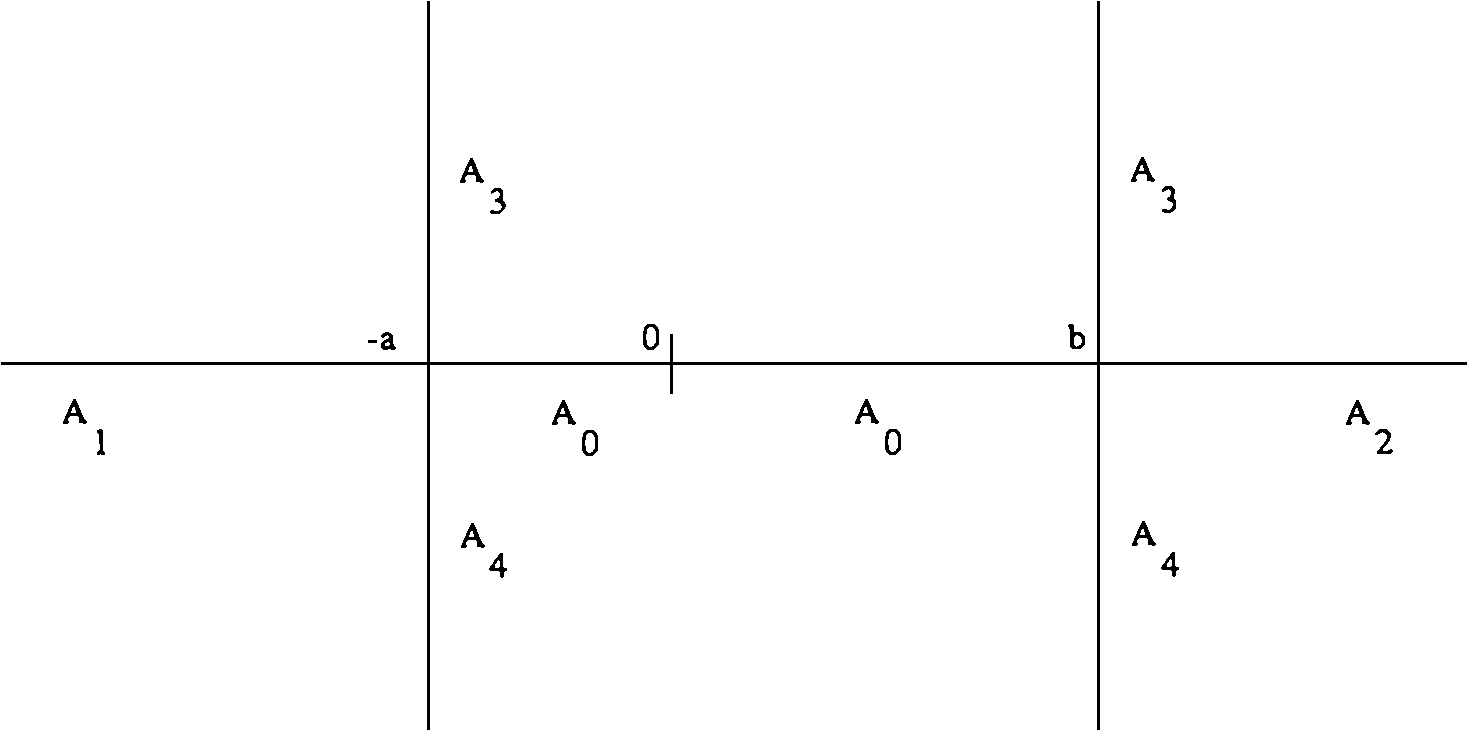
\includegraphics{Images/Img10.png}
    \caption{The sets $A_i$, $i=0,\ldots,4$.}
    \label{fig:ch5_2.1}
\end{figure}

The reduced sequence completely describes the homotopy class for $f(Z_t)$ with $f(L_t)$ added on whenever $Z_t \in B(0,\epsilon)$, and for this curve to be homotopic to a point, it is necessary that the reduced sequence consist of the single entry $0$. So to prove our proposition, it suffices to prove that the number of $0$s in the reduced sequence tends to $\infty$, a.s. Define a block to be a portion of a reduced sequence starting and ending with a $0$ and with no $0$s in the middle.

Suppose our last block in the reduced sequence is $\ldots 03140$. In order to reduce the number of $0$s, the next block must be $04130$. By symmetry about the $y = 0$ line, we are equally likely to have $03140$, which increases the number of $0$s by one. Also, by the support theorem, there is positive probability bounded away from $0$ that the next block will be $03240$ or $04230$, each of which increases the number of $0$s. A similar symmetry argument can be given no matter what the last block is, and so there exists $\delta > 0$ such that
\[
    \P(\text{number of $0$s increases by}~1) \geq 1/2 + \delta
\]
and
\[
    \P(\text{number of $0$s decreases by}~1) \leq 1/2 - \delta.
\]
By Exercise \ref{ex:ch5_5}, the number of 0s increases to $\infty$, a.s.
\end{proof}

\index{Picard's theorem|)}

\subsecbkm{ch5_sec2.2}{Distortion theorem}

We now give a probabilistic proof of what is known as the distortion theorem\index{Distortion theorem} or Koebe's $1/4$ theorem\index{Koebe's $1/4$ theorem}.

\begin{theorem}\label{thm:ch5_2.3}
Suppose $f$ is analytic and one to one on $\D$ with $f(0) = 0$ and $|f'(0)| = 1$. Then there exists $a$ (not depending on $f$) such that $B(0,a) \subseteq \allowbreak f(\D)$.
\end{theorem}

The best constant possible is $a = 1/4$, which explains the name of the theorem. The Koebe function $f(z) = z/(1-z)^2$ shows that the constant is attained. We will give a probabilistic proof of Theorem \ref{thm:ch5_2.3}; the constant we obtain is not as good as the one obtained from an analytic proof.

First we need an elementary fact about one to one analytic functions.

\begin{lemma}\label{lem:ch5_2.4}
If $f$ is one to one on a domain $D$, then $f'$ never vanishes on $D$.
\end{lemma}

\begin{proof}
Suppose $f'$ vanishes at some point of $D$. Without loss of generality, let us suppose that the point is $0 \in D$, and by adding a constant, we may assume $f(0) = 0$. Then in a neighborhood of 0, $f(z) = z^ng(z)$ where $n$ is an integer greater than or equal to 2 and $g$ is analytic in this neighborhood with $g(0) \neq 0$. By continuity, $g$ is not zero in a neighborhood of $0$, and so we can define $g^{1/n}$ as a single-valued analytic function there. Let $h(z) = zg(z)^{1/n}$, and we have $f(z) = [h(z)]^n$ in a neighborhood of $0$. Note $h(0) = 0$ and $h'(0) = g(0)^{1/n} \neq 0$. Since $h'(0) \neq 0$, the inverse of $h$ exists in a neighborhood of $h(0)$ by the inverse function theorem. Thus if $\epsilon$ is a sufficiently small positive real and $\omega = e^{\im 2\pi/n}$, there exist distinct points $z_1$ and $z_2$ such that $h(z_1) = \epsilon$ and $h(z_2) = \epsilon\omega$. Then $f(z_1) = f(z_2) = \epsilon^n$, contradicting the fact that $f$ is one to one.
\end{proof}

Next we have the following lemma.

\begin{lemma}\label{lem:ch5_2.5}
Suppose $|f'(0)| = 1$. There exists $\delta$ independent of $f$ such that
\begin{equation}\label{eq:ch5_2.1}
    \P^0\Big(\int_0^{\tau} |f'(Z_s)|^2ds > \delta\Big) \geq \delta.
\end{equation}
\end{lemma}

\begin{proof}
Let
\[
    g(r) = \frac{1}{2\pi}\int_0^{2\pi} |f'(re^{\im\theta})|^2d\theta.
\]
Since $|f'|^2 = |\partial_xu|^2 + |\partial_yu|^2$ and $\partial_xu$ and $\partial_yu$ are both harmonic, then $|f'|^2$ is subharmonic. So
\[
    1 = |f'(0)|^2 \leq \E^0|f'(Z_{\tau_r})|^2 = \frac{1}{2\pi}\int_0^{2\pi} |f'(re^{\im\theta})|^2d\theta = g(r).
\]

Define $F(z) = |f'(z)|^2/g(|z|)$, where we set $g(0) = 1$. Then $F(0) = 1$, $F(z) \leq |f'(z)|^2$, and $(2\pi)^{-1}\int_0^{2\pi} F(re^{\im\theta})d\theta = 1$.

The Green function for $\D$ is given by Exercise \chapref[II.8]{ex:ch2_45}. Hence
\begin{align*}
    \E^0\int_0^\tau F(Z_s)ds &= \int_{\D} g_{\D}(0,z)F(z)dz \geq \int_{B(0,1/4)} g_{\D}(0,z)F(z)dz \\
    &\geq c\int_0^{1/4} \log(1/r)r\int_0^{2\pi} F(re^{\im\theta})d\theta dr \geq c_1.
\end{align*}
On the other hand, if $w \in \D$,
\[
    g_{\D}(w,z) \leq -c\log(|w-z|/2) \leq -c\log((|w|-|z|)/2),
\]
and so there exists $c_2$ such that for all $w \in \D$,
\begin{align*}
    \E^w\int_0^\tau F(Z_s)ds &= \int_{\D} g_{\D}(w,z)F(z)dz \\
    &\leq -c\int_0^1 r\log((r-|w|)/2)\int_0^{2\pi} F(re^{\im\theta})d\theta dr \leq c_2.
\end{align*}
If $A_t = \int_0^{t\wedge \tau} F(Z_s)ds$, then
\[
    \E^w[A_\infty - A_t\mid \FC_t] = \E^{Z_t}A_\infty \leq c_2.
\]
By Theorem \chapref[I]{thm:ch1_6.10} with $B = c_2$, there exists $c_3$ such that
\begin{equation}\label{eq:ch5_2.2}
    \sup_w \E^w\Big[\int_0^\tau F(Z_s)ds\Big]^2 \leq c_3.
\end{equation}

Then
\begin{align*}
    c_1 &\leq \E^0\int_0^\tau F(Z_s)ds = \E^0\Big[\int_0^\tau F(Z_s)ds; \int_0^\tau F(Z_s)ds \leq c_1/2\Big] \\
    &\qquad + \E^0\Big[\int_0^\tau F(Z_s)ds; \int_0^\tau F(Z_s)ds > c_1/2\Big] \\
    &\leq c_1/2 + \Big(\E^0\Big[\int_0^\tau F(Z_s)ds\Big]^2\Big)^{1/2}\Big(\P^0\Big(\int_0^\tau F(Z_s)ds > c_1/2\Big)\Big)^{1/2}.
\end{align*}
Using \eqref{eq:ch5_2.2},
\[
    \P^0\Big(\int_0\tau F(Z_s)ds > c_1/2\Big) \geq \frac{(c_1/2)^2}{c_3}.
\]
Since $|f'(z)|^2 \geq F(z)$, this proves the lemma.
\end{proof}

Now we are ready to prove Theorem \ref{thm:ch5_2.3}. The idea is that by the support theorem, $f(Z_t)$ will make a loop\index{Loop|(} around the outside of the ball of radius $a$ about $0$. Since $f(\D)$ is simply connected, this means the ball of radius $a$ must be contained in $f(\D)$. Here are the details.

% Note: it seems that \delta in the following proof refers to one in Lemma 2.5 and not 2.2. Also Lemma 2.1 is in fact Lemma 2.4

\begin{proof}[Proof of Theorem \ref{thm:ch5_2.3}]
Let $W_t$ be two-dimensional Brownian motion. Let $\delta$ be as in Lemma \ref{lem:ch5_2.5}. We will show
\begin{obs}\label{obs:ch5_2.3}
    \textit{There exists $a > 0$ such that $W_t$ makes a loop around $B(0,a)$ before time $\delta$ with probability at least $1-\delta/2$.}
\end{obs}

By making a loop around $B(0,a)$, we mean the graph of $\{W_s:0\leq s \leq \delta\}$ contains a closed curve $\gamma$ with $B(0,a)$ contained in one of the bounded components of $\gamma^c$.

Before showing \eqref{obs:ch5_2.3}, let us see how \eqref{obs:ch5_2.3} implies the theorem. Let $Z_t$ be two-dimensional Brownian motion in $\D$ and let $W_t$ be a two-dimensional Brownian motion that agrees with the time change of $f(Z_t)$ up to the first exit of $D$. By Lemma \ref{lem:ch5_2.5} and Theorem \ref{thm:ch5_1.1}, $W_t$ will not have exited $D$ by time $\delta$ with probability at least $\delta$. So by \eqref{obs:ch5_2.3}, with probability at least $\delta/2$ the graph of $\{W_s : 0 \leq s \leq \tau_D(W)\}$ will make a loop\index{Loop|)} around $B(0,a)$. This graph is the same as the graph of $\{f(Z_s) : 0 \leq s \leq \tau_D(Z)\}$. (Here $\tau_D(W)$ is the exit time of $D$ for $W$ and $\tau_{\D}(Z)$ is the exit time of $\D$ for $Z$.) It follows that $f(\D)$ contains a closed curve containing $B(0,a)$. Since $f$ is one to one, $f'$ is never $0$ by Lemma \ref{lem:ch5_2.4} and $f^{-1}$ is analytic. Since $f$ and $f^{-1}$ are both continuous, $f(\D)$ is simply connected. If there were $z \in B(0,a)$ that was not in $f(\D)$, that would contradict the fact that $f(D)$ is simply connected. Therefore $B(0,a) \subseteq f(\D)$.

We now show \eqref{obs:ch5_2.3}. There exists $r$ small such that
\begin{equation}\label{eq:ch5_2.4}
    \P^0(\tau_r>\delta)\leq \delta/4.
\end{equation}

Let $\psi(t)$ be a curve that starts at $1$, goes around the circumference of $B(0,1)$ twice, then goes from $1$ to $2$ along the positive real axis, and finally from $2$ to $1/4$ along the positive real axis. If $\epsilon = 1/16$, by the support theorem (Theorem \chapref[I]{thm:ch1_6.6}), there exists $\eta > 0$ such that the graph of Brownian motion started at $1$ will, with probability at least $\eta$, contain a closed curve that has $B(0,1/4)$ in its interior.

Let
\begin{align*}
    A_k = \{T_{\partial B(0,16^{-k}r/2)} &< T_{\partial B(0,8\cdot16^{-k}r)} ~\text{and the graph of} \\
    &\{W_s, s \in [0,T_{\partial B(0,16^{-k}r/2)} \wedge T_{\partial B(0,8\cdot16^{-k}r)}]\} \\
    &\text{contains a closed curve containing}~B(0,16^{-k}r/4)\}.
\end{align*}
By scaling, if $|z| = 16^{-k}r$, then $\P^z(A_k) \geq \eta$, or $\P^z(A_k^c) \leq 1-\eta$. By the strong Markov property at time $T_{\partial B(0,16^{-4k}r)}$,
\[
    \P^0(A_4^c \cap A_8^c \cap \cdots \cap A_{4k}^c) \leq (1-\eta)\P^0(A_8^c \cap \cdots \cap A_{4k-4}^c).
\]
By induction,
\[
    \P^0(A_4^c \cap A_8^c \cap \cdots \cap A_{4k}^c) \leq (1-\eta)^k.
\]
If we take $k$ large enough so that $(1-\eta)^k \leq \delta/4$ and combine with \eqref{eq:ch5_2.4}, we have \eqref{obs:ch5_2.3} with $a = 16^{-4k}r/4$.
\end{proof}

\begin{corollary}\label{cor:ch5_2.6}
Suppose $f$ is one to one and analytic on $\D$, $z \in \D$. Then
\[
    \dist(f(z),\partial f(\D)) \leq a^{-1}|f'(z)|(1-|z|).
\]
\end{corollary}

\begin{proof}
Let $r = a^{-1}|f'(z)|(1-|z|)$ and suppose $r < \dist(f(z),\partial f(\D))$. Apply the distortion theorem to $f^{-1}$ and $B(f(z),r)$. By scaling,
\[
    B\big(z,ar/|(f^{-1})'(f(z))|\big) \subseteq f^{-1}\big(B(f(z),r)\big),
\]
or
\[
    f\big(B(z,ar/|f'(z)|)\big) \subseteq B(f(z),r).
\]
So we have $f(B(z,1-|z|)) \subseteq B(f(z),r)$. If $w \to z/|z|$ with $w \in B(z,1-|z|)$, then $f(w) \to \partial \D$ yet $f(w) \in B(f(z),r)$. This contradicts $r < \dist(f(z),\partial f(\D))$.
\end{proof}

\section{Boundary behavior of analytic functions}\label{ch5_sec3}

\subsecbkm{ch5_sec3.1}{Nontangential limits}
\index{Nontangential limit|(}

We are going to look at the boundary behavior of functions analytic in the unit disk $\D$. First of all, a great deal can be said simply by looking at the real and imaginary parts of $f$. Both are harmonic functions and the results of Chap.\ \ref{ch4} can be easily modified to deal with the case $d = 2$ and the unit disk instead of the half-space. One can go through the proofs and make the appropriate modifications. Or, since we are looking at analytic functions, we can simply use a conformal mapping argument.

However, in preparation for describing some of the behavior peculiar to analytic functions, we will need to know that a harmonic function $u$ converges nontangentially the same places $u(Z_t)$ converges. Let $C_\theta$ be the convex hull of $\{e^{\im\theta}\} \cup B(0,1/4)$, the Stolz domain with vertex at $e^{\im\theta}$, and let
\begin{equation}\label{eq:ch5_3.1}
    L_u = \{\theta : \lim_{z \in C_\theta, z \to e^{\im\theta}} u(z)~\text{exists}\}.
\end{equation}
For the probabilistic analog, let
\begin{equation}\label{eq:ch5_3.2}
    L_u = \{\theta : \lim_{t \to \tau} u(Z_t)~\text{exists}~\P_\theta^0-\text{a.s.}\}.
\end{equation}
We are assuming $u$ is harmonic, but not necessarily positive and $\P_\theta^0$\index{P5@$\P_\theta^z$} is the law of Brownian motion conditioned to exit $\D$ at $e^{\im\theta}$, or phrased another way, the law of Brownian motion $h$-path transformed by the Poisson kernel with pole at $e^{\im\theta}$.

\mpagebreak

First we show $\LC_u\subseteq L_u$ up to a set of measure $0$. The analog of this for $d\ge 2$ is not true; see \cite{Durrett1984}.

\begin{proposition}\label{prop:ch5_3.1}
Almost every $\theta \in \LC_u$ is in $L_u$. Moreover for almost every $\theta \in \LC_u$,
\[
    \lim_{t\to\tau} u(Z_t) = \lim_{z\in C_\theta,z\to e^{\im\theta}} u(z), \qquad \P_\theta^0-\text{a.s.}
\]
\end{proposition}

\begin{proof}
Fix $\theta \in \LC_u$. By the zero-one law (Theorem \chapref[III]{thm:ch3_2.9}), $\lim_{t\to\tau} u(Z_t)$ is a constant, say $\ell$, $\P_\theta^0$-a.s. Suppose there exist $z_1,z_2,\dots$ in $C_\theta$ converging to $e^{\im\theta}$ with $u(z_n) - \ell > \epsilon$ for some $\epsilon > 0$. We will show there exists $c$ independent of $n$ such that
\begin{equation}\label{eq:ch5_3.3}
    \P_\theta^0(Z_t~\text{makes a loop around}~z_n) \geq c.
\end{equation}
As in Sect.\ \chapref[V]{ch5_sec2}, by ``$Z_t$ makes a loop around $z_n$,'' we mean that the path of $Z_t$, $t < \tau$, contains a closed curve $\gamma_n$ with $z_n$ inside the region enclosed by $\gamma_n$. Before proving \eqref{eq:ch5_3.3}, let us show that \eqref{eq:ch5_3.3} implies the proposition. Since $u(Z_t)$ converges to $\ell$, we can take $\delta$ small enough so that $u(Z_t) \leq \ell + \epsilon/2$ if $t > \tau - \delta$ ($\gamma_n$ and $\delta$ are random, of course). Since $Z_t \to e^{\im\theta}$, $\P_\theta^0$-a.s., $\gamma_n$ is contained in the graph of $\{Z_t : \tau - \delta < t < \tau\}$ if $n$ is large enough. By the maximum principle, since $z_n$ is in the region enclosed by $\gamma_n$, $u(z_n) \leq \sup_{\gamma_n} u$, which will be less than $\ell + \epsilon/2$ if $n$ is large enough, a contradiction. Therefore $\limsup_n u(z_n) \leq \ell$. The $\liminf$ is treated similarly.

So we need to prove \eqref{eq:ch5_3.3}. This is a consequence of the support theorem. Let us suppose for simplicity that $r_n = 1 - |z_n| < 1/4$, the other case being easier, and suppose $\theta = 0$.

Let $h_\theta(z)$ be the Poisson kernel for $\D$ with pole at $0$ (Theorem \chapref[II]{thm:ch2_1.17}). Let
\[
    L_n = \{(1 - r_n)e^{\im\theta} : -\pi r_n/16 < \theta < \pi r_n/16\}.
\]
Then
\begin{align}\label{eq:ch5_3.4}
    \P_0^0(Z_{\tau(1-r_n)} \in L_n) &= \frac{\E^0[h_0(Z_{\tau(1-r_n)}); Z_{\tau(1-r_n)} \in L_n]}{h_0(0)} \\
    &\geq cr_n^{-1}\P^0(Z_{\tau(1-r_n)} \in L_n) \geq c. \notag
\end{align}

Fix $z \in L_n$. Let $\psi_n$ be the curve that goes at constant speed from $z$ toward the origin a distance $r_n/2$, moves clockwise along $\partial B(0,1-3r_n/2)$ an angle $\pi r_n/4$, moves radially away from the origin a distance $r_n$, moves counterclockwise along $\partial B(0,1-r_n/2)$ an angle $\pi r_n/2$, moves toward the origin a distance $3r_n/4$, and then moves clockwise along $\partial B(0,1-5r_n/4)$ an angle $\pi r_n$. Let $\epsilon_n = r_n/16$. Let $A_n = \{\sup_{s\leq\sqrt{r_n}} |Z_s - \psi_n(s)| < \epsilon_n\}$. By the support theorem (Theorem \chapref[I]{thm:ch1_6.6}) and scaling,
\[
    \P^z(Z_t~\text{makes a loop around}~z_n) \geq \P^z(A_n) \geq c.
\]
In fact, since $A_n$ is in $\FC_{\tau(1-r_n/4)\wedge T(\partial B(0,1-2r_n))}$ and $h_0(w)/h_0(v)$ is bounded above for $w,v \in B(0,1-r_n/4) - B(0,1-2r_n)$,
\begin{equation}\label{eq:ch5_3.5}
    \P_0^0(Z_t~\text{makes a loop around}~z_n) \geq \P_0^0(A_n) \geq c.
\end{equation}
By the strong Markov property, \eqref{eq:ch5_3.4} and \eqref{eq:ch5_3.5},
\begin{align*}
    \P_0^0(Z_t~&\text{makes a loop around}~z_n)  \\
    &\!\geq \E_0^0[\P^{Z_{\tau(1-r_n)}}(Z_t~\text{makes a loop around}~z_n); Z_{\tau(1-r_n)} \in L_n] \\
    &\!\geq c.
\end{align*}
This proves \eqref{eq:ch5_3.3}.
\end{proof}

The other direction, that $L_u$ is contained in $\LC_u$ almost everywhere works for any dimension. First we need a lemma due to Marcinkiewicz. Let $\sigma$ be normalized surface measure on $\partial\D$.

\begin{lemma}\label{lem:ch5_3.2}
Suppose $F$ is a closed subset of $\partial\D$. Then for almost every $x \in F$,
\begin{equation}\label{eq:ch5_3.6}
    I(x) = \int_{\partial\D} \frac{\dist(y,F)}{|x-y|^2} \sigma(dy) < \infty.
\end{equation}
\end{lemma}

The integral $I(x)$ is known as the integral of Marcinkiewicz\index{Marcinkiewicz integral}, and the analog of this lemma holds in the half-space for any $d$.

\begin{proof}
We show $I(x)$ is finite a.e.\ by showing $\int_{\partial\D\cap F} I(x)\sigma(dx) < \infty$. By Fubini's theorem, this is equal to
\[
    \int\int_F \frac{\dist(y,F)}{|x-y|^2}\sigma(dx)\,\sigma(dy).
\]
Note $\dist(y,F) = 0$ unless $y \notin F$. If $x \in F$ and $y \notin F$, then $|x-y|$ must be greater than $\dist(y,F)$. So the double integral is bounded by
\[
    2\int\int_{\dist(y,F)}^\infty \frac{dz}{z^2}\dist(y,F)\sigma(dy) = 2\int \sigma(dy) < \infty.
\]
\end{proof}

\begin{proposition}\label{prop:ch5_3.3}
Almost every $\theta$ in $L_u$ is also in $\LC_u$.
\end{proposition}

\begin{proof}
Fix $M$ and let $E = E_M = \{e^{\im\theta} : \sup_{z\in C_\theta} |u(z)| \leq M\}$. Let $G = \cup_{e^{\im\theta}\in E}C_\theta$. Then $|u| \leq M$ in $G$. $G$ is a sawtooth domain (cf.\ Fig.\ \chapref[IV]{fig:ch4_6.1}). Because $\sup_{z\in C_\theta} |u(z)|$ is a lower semicontinuous function, $E$ is closed. The key step is to show:

If $e^{\im\theta} \in E$ and
\mpagebreak
\begin{equation}\label{eq:ch5_3.7}
    \int \frac{\dist(e^{\im x},E)}{|e^{\im\theta}-e^{\im x}|^2}\sigma(dx) < \infty,
\end{equation}
then
\begin{equation}\label{eq:ch5_3.8}
    \P_\theta^0(\limsup_{t<\tau} |u(Z_t)| \leq M) = 1.
\end{equation}

To prove \eqref{eq:ch5_3.8} we first make four observations. By the Harnack inequality, there exists $c$ such that
\begin{equation}\label{eq:ch5_3.9}
    h_\theta(\rho e^{\im\phi}) \leq ch_\theta(se^{\im\alpha})
\end{equation}
if $\rho e^{\im\phi}, se^{\im\alpha} \in \partial G - \partial\D$ with $|\phi - \alpha| \leq (1-\rho)/2$. Second, by the support theorem, there exists $c$ such that
\begin{equation}\label{eq:ch5_3.10}
    \P^{\rho e^{\im\phi}}(|Z_\tau - e^{\im\phi}| \leq (1-\rho)/2) \geq c.
\end{equation}
Third, note that
\begin{equation}\label{eq:ch5_3.11}
    h_\theta(se^{\im\alpha}) \leq \frac{c(1-s)}{|se^{\im\alpha} - e^{\im\theta}|^2} \leq \frac{c\dist(e^{\im\alpha},E)}{|e^{\im\alpha} - e^{\im\theta}|^2}
\end{equation}
if $se^{\im\alpha} \in \partial G - \partial\D$. Fourth, if $z \in C_\theta$,
\begin{equation}\label{eq:ch5_3.12}
    \frac{h_\alpha(z)}{h_\theta(z)} = \frac{|z - e^{\im\theta}|^2}{|z - e^{\im\alpha}|^2} \leq c.
\end{equation}

If $e^{\im\phi} \notin E$, $\rho e^{\im\phi} \in \partial G - \partial\D$, and $|\alpha - \phi| \leq (1-\rho)/2$, then $e^{\im\alpha} \notin E$. For such $\alpha$ choose $s_\alpha$ such that $s_\alpha e^{i\alpha} \in \partial G - \partial\D$. Combining \eqref{eq:ch5_3.9}, \eqref{eq:ch5_3.10}, and \eqref{eq:ch5_3.11},
\begin{align}\label{eq:ch5_3.13}
    h_\theta(\rho e^{\im\phi}) &\leq ch_\theta(\rho e^{\im\phi})\P^{\rho e^{\im\phi}}(|Z_\tau - e^{\im\phi}| \leq (1-\rho)/2) \\
    &\leq ch_\theta(\rho e^{\im\phi})\int_{\phi-(1-\rho)/2}^{\phi+(1-\rho)/2} h_\alpha(\rho e^{\im\phi})d\alpha \notag \\
    &\leq c\int_{\phi-(1-\rho)/2}^{\phi+(1-\rho)/2} h_\theta(s_\alpha e^{\im\alpha}) h_\alpha(\rho e^{\im\phi})d\alpha \notag \\
    &\leq c\int_{\phi-(1-\rho)/2}^{\phi+(1-\rho)/2} \frac{\dist(e^{\im\alpha},E)}{|e^{\im\alpha} - e^{\im\theta}|^2}h_\alpha(\rho e^{\im\phi})d\alpha. \notag
\end{align}

If $r>0$ and $|\rho e^{\im\phi} - e^{\im \theta}|$, then $\phi+(1-\rho)/2\leq \theta + cr$ and $\phi-(1-\rho)/2\geq \theta - cr$, So using \eqref{eq:ch5_3.12}, \eqref{eq:ch5_3.13}, and the fact that $h_\theta(Z_{t\wedge\tau})$ is a martingale, if $z \in C_\theta$,

\mpagebreak
\begin{align}\label{eq:ch5_3.14}
    \P_\theta^z(\tau_G < \tau,\,&|Z_{\tau_G} - e^{\im\theta}| < r) \\
    &= \E^z\big[h_\theta(Z_{\tau_G}); \tau_G < \tau,|Z_{\tau_G} - e^{\im \theta}| < r\big]/h_\theta(z) \notag \\
    &\leq c\E^z \int_{\theta-cr}^{\theta+cr} \frac{\dist(e^{\im\alpha},E)}{|e^{\im\alpha} - e^{\im\theta}|^2}\frac{h_\alpha(Z_{\tau_G})}{h_\theta(z)} d\alpha \notag \\
    &\leq c\int_{\theta-cr}^{\theta+cr} \frac{\dist(e^{\im\alpha},E)}{|e^{\im\alpha} - e^{\im\theta}|^2}\frac{h_\alpha(z)}{h_\theta(z)} d\alpha \notag \\
    &\leq c\int_{\theta-cr}^{\theta+cr} \frac{\dist(e^{\im\alpha},E)}{|e^{\im\alpha} - e^{\im\theta}|^2} d\alpha. \notag
\end{align}
Since $\theta$ satisfies \eqref{eq:ch5_3.7}, there exists $r$ such that the right-hand side of \eqref{eq:ch5_3.14} is less than $1/2$. Taking $z \in C_\theta$ with $z$ sufficiently close to $e^{\im\theta}$,
\[
    \P_\theta^z(|Z_{\tau_G} - e^{\im\theta}| > r) \leq 1/4.
\]
Hence $\P_\theta^z(\tau_G < \tau) \leq 3/4$. If $\tau_G = \tau$, then $u(Z_t)$ does not hit $G^c$ before $\partial\D$, and $\sup_{t<\tau} |u(Z_t)| \leq M < \infty$. So $\P_\theta^z(\limsup_{t<\tau} |u(Z_t)| \leq M) \geq 1/4$. The zero-one law (Theorem \chapref[III]{thm:ch3_2.9}) implies \eqref{eq:ch5_3.8}.

To complete the proof, by Lemma \ref{lem:ch5_3.2} and \eqref{eq:ch5_3.8}, for almost every $\theta \in E_M$ we have
\begin{equation}\label{eq:ch5_3.15}
    \P_\theta^0(\sup_{t<\tau} |u(Z_t)| < \infty) = 1.
\end{equation}
Since clearly $L_u \subseteq \cup_{M=1}^\infty E_M$, \eqref{eq:ch5_3.15} holds for almost every $\theta \in L_u$. By Proposition \chapref[III]{prop:ch3_2.7},
\[
    \P^0(\sup_{t<\tau}|u(Z_t)|<\infty, Z_{\tau}\in L_u)=\P^0(Z_{\tau}\in L_u).
\]
By Exercise \ref{ex:ch5_8},
\[
    \P^0(Z_\tau \in L_u) = \P^0(\lim_{t\to\tau} u(Z_t)~\text{exists}, Z_\tau \in L_u),
\]
or for almost every $\theta \in L_u$, $\P_\theta^0(\lim_{t\to\tau} u(Z_t)~\text{exists}) = 1$. This is the assertion of the proposition.
\end{proof}

\index{Nontangential limit|)}

The above proposition has analogs in the half-space and for any dimension $d$. We took our Stolz domains to be the convex hull of $\{e^{\im \theta}\} \cup B(0,1/4)$. Of course, the $1/4$ could be replaced by any number between $0$ and $1$, and so our $C_\theta$ could have any aperture angle we desired between $0$ and $\pi$.

\subsecbkm{ch5_sec3.2}{Privalov theorem}

We can now easily prove some interesting results about the boundary behavior of analytic functions.

\begin{theorem}[Privalov\index{Privalov's theorem}]\label{thm:ch5_3.4}
\begin{enumerate}[wide, labelindent=0em, labelwidth=\parindent, labelsep = 0em]
\item If $\lim_{z\in C_\theta,z\to e^{\im\theta}} f(z) = 0$ on a set of $\theta$s of positive Lebesgue measure, then $f$ is identically $0$.
\item If $\lim_{z\in C_\theta,z\to e^{\im\theta}} |f(z)| = \infty$ on a set of $\theta$s of positive Lebesgue measure, then $f$ is identically infinite.
\end{enumerate}
\end{theorem}

\begin{proof}
(a) Suppose $f$ is not identically $0$. Then $f(Z_t)$ is a time change of two-dimensional Brownian motion. Since with probability one two-dimensional Brownian motion never hits $0$ and does not tend to $0$ as $t \to \infty$, then $\P^0(\lim_{t\to\tau} f(Z_t) = 0) = 0$. So $\{\theta : \P_\theta^0(\lim_{t\to\tau} f(Z_t) = 0) = 1\}$ must have Lebesgue measure $0$. By Proposition \ref{prop:ch5_3.3}, $\{\theta : \lim_{z\in C_\theta,z\to e^{\im\theta}} f(z) = 0\}$ must also have Lebesgue measure $0$.

(b) is very similar, observing that two-dimensional Brownian motion does not tend to infinity in modulus as $t \to \infty$ (Proposition \chapref[I]{prop:ch1_5.8}).
\end{proof}

There is an interesting open problem concerning the analog of this in higher dimensions. Suppose $u$ is harmonic in $B(0,1)$ (or in a half-space) and $C^2$ (or even $C^\infty$) in $\overline{B(0,1)}$. Let
\begin{equation}\label{eq:ch5_3.16}
    A = \{\theta : \lim_{z\in B(0,1),z\to e^{\im\theta}} u(z) = 0, \lim_{z\in B(0,1),z\to e^{\im\theta}} \nabla u(z) = 0\}.
\end{equation}
If $|A| > 0$, must $u$ be identically $0$? Amazingly enough this need not be true if we only require $u \in C^{1+\alpha}(\overline{B(0,1)})$ for some $\alpha > 0$ (see \cite{BourgainWolff1990}). The question is still open for $u \in C^2$ or even $u \in C^\infty$.

\subsecbkm{ch5_sec3.3}{Plessner's theorem}

After some preliminary lemmas we can also prove Plessner's theorem\index{Plessner's theorem|(}.

\begin{lemma}\label{lem:ch5_3.5}
For almost every $\omega$, either $\lim_{t\to\tau} f(Z_t(\omega))$ exists or for every $\epsilon$, the set $\{f(Z_t(\omega)), t \in [\tau(\omega)-\epsilon,\tau(\omega))\}$ is dense in $\C$.
\end{lemma}

\begin{proof}
Let $U_t = \Re f(Z_{t\wedge\tau})$, $V_t = \Im f(Z_{t\wedge\tau})$. By the Cauchy-Riemann equations, $\lrang{U}_\tau = \lrang{V}_\tau$. For almost every $\omega$ for which $\lrang{U}_\tau < \infty$, we know $\lim_{t\to\tau} U_t$ and $\lim_{t\to\tau} V_t$ exist by Exercise \ref{ex:ch5_8}. If $\omega$ is such that $\lrang{U}_\tau = \lrang{V}_\tau = \infty$, $f(Z_t)$ is the time change of a two-dimensional Brownian motion path. Since two-dimensional Brownian motion is neighborhood recurrent, $f(Z_t)$ hits every neighborhood in $\C$ infinitely often.
\end{proof}

\begin{lemma}\label{lem:ch5_3.6}
If $A$ is a Borel subset of $\D$,
\[
    \P^z\big(Z_\tau \in A, Z_t \in \cup_{e^{\im\theta}\in A}C_\theta~\text{for all}~t \in [\tau-\epsilon,\tau)\big) \to \P^z(Z_\tau \in A)
\]
as $\epsilon \to 0$.
\end{lemma}

\begin{proof}
Let $h(z) = \P^z(Z_\tau \in A)$. If $w \notin \cup_{e^{\im\theta}\in A}C_\theta$, there exists $\delta > 0$ such that $\P^w(Z_\tau \notin A) > \delta$ by the support theorem (cf.\ proof of Proposition \chapref[IV]{prop:ch4_6.3}). So $h(z) \leq 1-\delta$ on $(\cup_{e^{\im\theta}\in A}C_\theta)^c$. Since $h(z) = \E^z1_A(Z_\tau)$ is harmonic, $h(Z_t) \to 1_A(Z_\tau)$, a.s., by the martingale convergence theorem. Then
\begin{align*}
    \big(Z_\tau \in A, Z_t \notin \cup_{e^{\im\theta}\in A}C_\theta~\text{i.o.}\big) &\subseteq \big(Z_\tau \in A, h(Z_t) < 1-\delta~\text{i.o.}\big) \\
    &\subseteq \big(Z_\tau \in A, \lim_{t\to\tau} h(Z_t) < 1-\delta\big),
\end{align*}
and the last event has probability $0$.
\end{proof}

\begin{theorem}[Plessner]\label{thm:ch5_3.7}
For almost every $\theta$, either $f$ has a nontangential limit at $e^{\im\theta}$ or $f(C_\theta)$ is dense in $\C$.
\end{theorem}

\begin{proof}
Let $L_f = \{\theta :~\text{the nontangential limit of}~f~\text{exists at}~e^{\im\theta}\}$. Suppose $|L_f^c| > 0$ and $A \subseteq L_f^c$ with $|A| > 0$. Then for a.e.\ $\theta$ with $e^{\im\theta} \in A$, $\theta \notin L_f$, or
\[
    \P_\theta^0\big(\lim_{t\to\tau} f(Z_t)~\text{exists}\big) = 0.
\]
% Note: it seems that the next sentence refers to Lemma 3.5
By Proposition \chapref[III]{prop:ch3_2.7}, $\P^0(\lim f(Z_t)~\text{exists}, Z_\tau \in A) = 0$. Then by Lemma \ref{lem:ch5_3.5},
\begin{align*}
    \P^0&\big(\{f(Z_t), t \in [\tau-\epsilon,\tau)\}~\text{is not dense in}~\C~\text{for all}~\epsilon, Z_\tau \in A\big) \\
    &\leq \P^0\big(\{f(Z_t), t \in [\tau-\epsilon,\tau)\}~\text{is not dense in}~ \C~\text{for all}~\epsilon, \\
    &\qquad\qquad\qquad\lim f(Z_t)~\text{does not exist}\big) \\
    &\qquad\qquad+ \P^0(\lim f(Z_t)~\text{exists}, Z_\tau \in A) = 0.
\end{align*}
By Lemma \ref{lem:ch5_3.6}, on the set $(Z_\tau \in A)$ we know that $Z_t$ will be in $\cup_{e^{\im\theta}\in A}C_\theta$ for all $t$ sufficiently close to $\tau$. Hence $f(\cup_{e^{\im\theta}\in A}C_\theta)$ must be dense in $\C$.

This is true for all $A \subseteq L_f^c$. Let $D_\theta = f(C_\theta)$. Let $\{Q_i\}$ be the collection of balls with rational radii and centers that have rational real and imaginary parts. So $\{Q_i\}$ is a basis for $\C$. If $|\{\theta \in L_f^c : D_\theta \neq \C\}| > 0$, then for some $i_0$, $|\{\theta \in L_f^c : D_\theta \cap Q_{i_0} = \emptyset\}| > 0$. If we let $A = \{\theta \in L_f^c : D_\theta \cap Q_{i_0} = \emptyset\}$, then $f(\cup_{e^{\im\theta}\in A}C_\theta)$ does not intersect $Q_{i_0}$, a contradiction. Hence for almost every $\theta \in L_f^c$, $f(C_\theta)$ is dense in $\C$.
\end{proof}

\index{Plessner's theorem|)}

A stronger statement is McMillan's twist theorem\index{McMillan twist theorem}. This says that for almost every $\theta$ either $f'$ has a nontangential limit at $e^{\im\theta}$ or else
\begin{align}\label{eq:ch5_3.17}
\limsup_{z\in C_\theta,z\to e^{\im\theta}} \arg(f(z) - f(e^{\im\theta})) &= \infty \qquad \text{and} \\
\liminf_{z\in C_\theta,z\to e^{\im\theta}} \arg(f(z) - f(e^{\im\theta})) &= -\infty \notag
\end{align}
($\arg w$, the argument of $w$, is the imaginary part of $\log w$); see \cite{Pommerenke1992} for a proof.

\subsecbkm{ch5_sec3.4}{Nevanlinna class}

If $\sup_{r<1} \int_0^{2\pi} |f(re^{\im\theta})|^p d\theta < \infty$ for some $p \in (0,\infty)$, then by analogy to the half-space case, we say that $f \in H^p$. If $f \in H^1$, then by Theorem \chapref[IV]{thm:ch4_6.10}, $f$ then has nontangential limits a.e. However, in two dimensions, less is needed. If $\sup_{r<1} \int_0^{2\pi} \log^+ |f(re^{\im\theta})|d\theta < \infty$, we say that $f$ is in the Nevanlinna class\index{Nevanlinna class}. The most interesting property of such $f$s is a decomposition into simpler analytic functions (see \cite{Garnett1981}). A consequence of this decomposition is that $f$s in the Nevanlinna class have nontangential limits. We give a probabilistic proof.

\begin{proposition}\label{prop:ch5_3.8}
If $f$ is in the Nevanlinna class, then $f$ has nontangential limits for almost every $\theta$.
\end{proposition}

\begin{proof}
By Lemma \ref{lem:ch5_1.7}, $\log^+ |f(z)|$ is subharmonic, so $\log^+ |f(Z_t)|$ is a nonnegative submartingale. It is uniformly bounded in $L^1$ since
\[
    \E^0\log^+ |f(Z_{t\wedge\tau})| \leq \sup_{r<1}\E^0\log^+ |f(Z_{t\wedge\tau_r})| \leq \sup_{r<1}\E^0\log^+ |f(Z_\tau)|
\]
by Fatou's lemma and optional stopping.
\[
    \sup \E^0\log^+ |f(Z_{\tau_r})| = \sup_{r<1} \frac{1}{2\pi}\int_0^{2\pi} \log^+ |f(re^{\im\theta})|d\theta
\]
is finite since $f$ is in the Nevanlinna class, and we have the uniform boundedness in $L^1$. Therefore $\log^+ |f(Z_t)|$ converges almost surely, and in particular, $\sup_{t<\tau} |f(Z_t)| < \infty$, a.s.

For each $M$, let $G_M = \{\cup C_\theta : \sup_{z\in C_\theta} |f(z)| \leq M\}$. By the finiteness of $\sup |f(Z_t)|$, $\P^0(\tau_{G_M} < \tau) \to 0$ as $M \to \infty$. If $f = u+\im v$, then $u$ and $v$ are both bounded on $G_M$, so $u(Z_t)$ and $v(Z_t)$ both converge as $t \to \tau \wedge \tau_{G_M}$. With the above this implies that $u(Z_t)$ and $v(Z_t)$ converges a.s.\ as $t \to \tau$. By Proposition \ref{prop:ch5_3.1}, this implies the result.
\end{proof}

\subsecbkm{ch5_sec3.5}{LIL for Bloch functions}

A Bloch function\index{Bloch function|(} is a function $f$ that is analytic in $\D$ with
\begin{equation}\label{eq:ch5_3.18}
    \|f\|_B = |f(0)| + \sup_{z\in\D}(1-|z|)|f'(z)| < \infty.
\end{equation}
Thus, these are analytic functions whose derivative at $z$ grows no faster than the distance from $z$ to the boundary. By Corollary \chapref[II]{cor:ch2_1.4}, bounded analytic functions are Bloch functions. Another example of a Bloch function is the lacunary series\index{Lacunary series} $f(z) = \sum_{k\geq 0} z^{2^k}$ (Exercise \ref{ex:ch5_9}). (This series is called lacunary because of the ``lacuna'' or ``holes'' in the sequence of exponents of $z$.)

The important members of the Bloch class for us are given by the following.

\begin{proposition}\label{prop:ch5_3.9}
If $f$ is one to one on $\D$, then $\log f'$ is a Bloch function.
\end{proposition}

\begin{proof}
Let us normalize $f$ so that $f(0) = 0$ and $f'(0) = 1$. By the distortion theorem, $f(\D) \supseteq B(0,a)$, so $f^{-1}$ is one to one on $B(0,a)$. By applying the distortion theorem to $f^{-1}$ and $B(0,a)$, $f^{-1}(B(0,a)) \supseteq B(0,a^2)$, or $f(B(0,a^2)) \subseteq B(0,a)$. This can be rephrased by saying $f$ is bounded by $a$ on $B(0,a^2)$. By Corollary \chapref[II]{cor:ch2_1.4} applied to the real and imaginary parts of $f(z)$,
\[
    |f''(0)| \leq \frac{c}{(a^2)^2} \sup_{z\in B(0,a^2)} |f(z)| \leq \frac{c}{a^3} = c.
\]
By our normalization,
\[
    f(z) = z + b_2z^2 + b_3z^3 + \cdots.
\]
So what we have shown is that $|b_2| \leq c$, $c$ independent of $f$.

The mapping $z \to (z + z_0)/(1 + \overline{z_0}z)$ is one to one from $\D$ to itself and maps 0 to $z_0$. Hence
\[
    h(z) = \frac{f((z + z_0)/(1 + \overline{z_0}z)) - f(z_0)}{(1-|z_0|^2)f'(z_0)}
\]
is one to one on $\D$ and
\[
    h(z) = z + \Big(\frac{1}{2}(1-|z_0|^2)\frac{f''(z_0)}{f'(z_0)} - \overline{z_0}\Big)z^2 + \cdots.
\]
Therefore,
\[
    \Big|\frac{1}{2}(1-|z_0|^2)\frac{f''(z_0)}{f'(z_0)} - \overline{z_0}\Big| \leq c.
\]
Since $|z_0| \leq 1$,
\[
    (1-|z_0|)|f''(z_0)/f'(z_0)| \leq c,
\]
$c$ independent of $f$. This is the same as saying $\log f'$ is in the Bloch class.
\end{proof}

It is not hard to show that if $f$ is one to one on $\D$ with $f(0) = 0$, $f'(0) = 1$, then $|f''(0)| \leq 2$. The Bieberbach conjecture\index{Bieberbach conjecture}, proved by \cite{deBranges1985}, is the assertion that the $n$th coefficient in the Taylor expansion of $f$ about $0$ is bounded in absolute value by $n$.

We will show Makarov's law of the iterated logarithm\index{Makarov's law of the iterated logarithm|(} for Bloch functions. In the next section we will use it to settle a question about harmonic measure.

\begin{theorem}\label{thm:ch5_3.10}
Suppose $f$ is a Bloch function\index{Bloch function|)} with $\|f\|_B \leq 1$. There exists $\beta$ not depending on $f$ such that
\begin{equation}\label{eq:ch5_3.19}
    \limsup_{r\to 1} \frac{|f(re^{\im   \theta})|}{\sqrt{\log(1/(1-r))\log\log\log(1/(1-r))}} \leq \beta
\end{equation}
\mpagebreak
for almost all $\theta$.
\end{theorem}

By being a little more careful than we will be, one can show the result for $\beta = 2$. There is no lower bound for the $\limsup$; if $f$ is bounded, for example, the $\limsup$ is zero.

The proof will be broken up into several steps. In $\D$ the appropriate substitute for the $g_\lambda^*$ function of \chapeqref[IV]{eq:ch4_4.2} is
\[
    g^*(f)(\theta) = \Big(\E_\theta^0\Big[\int_0^\tau |f'(Z_s)|^2 ds\Big]\Big)^{1/2}.
\]

\begin{proposition}\label{prop:ch5_3.11}
Let $f$ be analytic with $g^*(f)$ bounded. Then
\[
    \frac{1}{2\pi}\int_0^{2\pi} e^{\lambda(f(e^{\im\theta})-f(0))} d\theta \leq e^{\lambda^2\|g^*(f)\|_\infty^2/2}.
\]
\end{proposition}

\begin{proof}
Let us normalize so that $f(0) = 0$ and $\|g^*(f)\|_\infty = 1$. Since $Z_\tau$ has a uniform distribution on $\partial\D$ under $\P^0$,
\begin{align*}
    \frac{1}{2\pi}\int_0^{2\pi} &e^{\lambda f(e^{\im\theta})-\lambda^2(g^*(f)(\theta))^2/2} d\theta \\
    &= \E^0\exp\Big(\lambda f(Z_\tau) - \frac{\lambda^2}{2}\E_{Z_\tau}^0\Big[\int_0^\tau |f'(Z_s)|^2 ds\Big]\Big) \\
    &= \E^0\exp\Big(\E_{Z_\tau}^0\Big[\lambda f(Z_\tau) - \frac{\lambda^2}{2}\int_0^\tau |f'(Z_s)|^2 ds\Big]\Big).
\end{align*}
By Jensen's inequality, this is less than
\[
    \E^0\E_{Z_\tau}^0\Big[\exp\Big(\lambda f(Z_\tau) - \frac{\lambda^2}{2}\int_0^\tau |f'(Z_s)|^2 ds\Big)\Big].
\]
By Proposition \chapref[III]{prop:ch3_2.7}, this is equal to
\begin{align*}
    \E^0\Big[\Big(\lambda f(Z_\tau) &- \frac{\lambda^2}{2}\int_0^\tau |f'(Z_s)|^2ds\Big)\Big] \\
    &= \E^0[\exp(\lambda f(Z_\tau) - \lambda^2\lrang{f(Z)}_\tau/2)] = 1.
\end{align*}
Since $g^*(f)$ is bounded by $1$,
\[
    \frac{1}{2\pi}\int_0^{2\pi} e^{\lambda f(e^{\im\theta})}d\theta \leq e^{\lambda^2/2}.
\]
\end{proof}

Next suppose $f$ is a Bloch function with $\|f\|_B \leq 1$. Let $f_r(e^{\im\theta}) = f(re^{\im\theta})$, denote the extension of $f_r$ by $f_r$ also, and let
\mpagebreak
\[
    f_r^*(\theta) = \sup_{0\leq s\leq r} |f_r(e^{\im\theta})|.
\]

We have the following.

\begin{proposition}\label{prop:ch5_3.12}
There exist $c_1$ and $c_2$ such that
\[
    |\{\theta : f_r^*(\theta) > \alpha\}| \leq c_1\exp\Big(-\frac{\alpha^2}{c_2\log(1/(1-r))}\Big).
\]
\end{proposition}

\begin{proof}
Let us first calculate $g^*(f_r)$.
\begin{align*}
    (g^*(f_r)(\theta))^2 &= \E_\theta^0\Big[\int_0^\tau |f'_r(Z_s)|^2ds\Big] \\
    &= r^2\E_\theta^0\Big[\int_0^\tau |f'(rZ_s)|^2 ds\Big] \\
    &\leq r^2\E_\theta^0\Big[\int_0^\tau \frac{ds}{(1-r|Z_s|)^2}\Big]
\end{align*}
since $f$ is a Bloch function. Since $h_\theta(z)$, the Poisson kernel with pole at $e^{\im\theta}$, is constant in $\theta$ when $z = 0$ and $h_\theta(Z_s)$ is a martingale, this is
\[
    cr^2\E^0\Big[\int_0^\tau \frac{ds}{(1-r|Z_s|)^2}h_\theta(Z_\tau)\Big] = cr^2\E^0\Big[\int_0^\tau \frac{h_\theta(Z_s)}{(1-r|Z_s|)^2}ds\Big].
\]
Using the Green function for $\D$, this is equal to
\begin{align*}
    cr^2\int_\D \log(1/|z|) &h_\theta(z)\frac{dz}{(1-r|z|)^2} \\
    &= cr^2\int_0^1\int_0^{2\pi} s\log(1/s)\frac{1}{(1-rs)^2}h_\theta(se^{\im\phi})d\phi\,ds \\
    &= cr^2\int_0^1 s\log(1/s)\frac{ds}{(1-rs)^2},
\end{align*}
where in the last equality we used the fact that $\int_0^{2\pi} h_\theta(se^{\im\phi})d\phi$ is constant in $\theta$ by rotational invariance. We have
\[
    cr^2\int_0^1 \frac{s\log(1/s)ds}{(1-rs)^2} \leq cr\int_0^1 \frac{ds}{1-rs} = c\log\frac{1}{1-r}.
\]
So $\|g^*(f_r)\|_\infty^2 \leq c\log(1/(1-r))$.

Next $\|f_r^*\|_p^p \leq c^p\|f_r\|_p^p$ by Exercise \chapref[IV.8]{ex:ch4_3}. Therefore
\mpagebreak
\begin{align*}
    \int_0^{2\pi} e^{\lambda f_r^*(\theta)}d\theta &= \sum_{p=0}^{\infty}\int_0^{2\pi} \frac{\lambda^p}{p!}|f_r^*(\theta)|^p d\theta \\
    &\leq \sum_{p=0}^{\infty}\int_0^{2\pi} \frac{\lambda^pc^p}{p!}|f_r(e^{\im\theta})|^pd\theta \\
    &\leq \int_0^{2\pi} e^{\lambda c|f_r(e^{\im\theta})|}d\theta.
\end{align*}
By Proposition \ref{prop:ch5_3.11}, this is less than
\[
    \exp\Big(\lambda^2c^2\|g^*(f_r)\|_\infty^2/2\Big) = \exp\Big(\lambda^2c^2\log(1/(1-r))/2\Big).
\]
Now use Chebyshev's inequality:
\[
    |\{\theta : f_r^*(\theta) > \alpha\}| = |\{\theta : e^{\lambda f_r^*(\theta)} > e^{\lambda\alpha}\}| \leq e^{-\lambda\alpha}\int_0^{2\pi} e^{\lambda f_r^*(\theta)}d\theta.
\]
Letting $\lambda = \alpha/c^2\log(1/(1-r))$, we obtain our result.
\end{proof}

\begin{proof}[Proof of Theorem \ref{thm:ch5_3.10}]
This is standard (cf.\ Exercise \chapref[I.8]{ex:ch1_4}). Let $r_n = 1-\exp(-2^n)$, let $\ell_n = \log(1/(1-r_n)) = 2^n$, let $c_2$ be as in Proposition \ref{prop:ch5_3.12}, and let
\[
    B_n = \{\theta : f_{r_n}^*(e^{\im\theta}) > 2(c_2\ell_n\log\log\ell_n)^{1/2}\}.
\]
By Proposition \ref{prop:ch5_3.12}, $|B_n| \leq cn^{-4}$. By the Borel-Cantelli lemma, $|(B_n~\text{i.o.})|\allowbreak = 0$. If $|f_r(e^{\im\theta})| > 4(c_2\log(1/(1-r))\log\log\log(1/(1-r)))^{1/2}$ for some $r$, then for some $r_n$, $\theta \in B_n$. The result follows with $\beta = 4c_2^{1/2}$.
\end{proof}

There are generalizations of Theorem \ref{thm:ch5_3.10} to harmonic functions where the distance to the boundary is replaced by expressions involving the area functional. See \cite{BanuelosKlemesMoore1988,BanuelosKlemesMoore1990} and \cite{BanuelosMoore1989a,BanuelosMoore1989b}.

\index{Makarov's law of the iterated logarithm|)}

\section{Harmonic measure}\label{ch5_sec4}

\subsecbkm{ch5_sec4.1}{Beurling's projection theorem}

Recall harmonic measure\index{Harmonic measure} is the hitting distribution of Brownian motion: if $E \subseteq \partial D$ and $x_0 \in D$,
\begin{equation}\label{eq:ch5_4.1}
    \omega^{x_0}(E) = \P^{x_0}(X_{\tau_D} \in E).
\end{equation}
By the Harnack inequality, harmonic measure relative to $x_0$ and harmonic measure relative to another point $x_1 \in D$ are mutually absolutely continuous and the density is bounded above and below by positive constants (see Theorem \chapref[III]{thm:ch3_2.6}).

\mpagebreak

We start by giving a proof of Beurling's projection theorem\index{Beurling projection theorem}. The circular projection of a set $E \subseteq \D$ is
\begin{equation}\label{eq:ch5_4.2}
    \gamma(E) = \{|z| : z \in E\}.
\end{equation}
$\gamma(E)$ is a subset of the positive real axis. Beurling's projection theorem\index{Beurling projection theorem|(} says that Brownian motion killed on exiting $\D$ is more likely to hit $E$ than $\gamma(E)$. Let $a = -1/2$.

\begin{theorem}\label{thm:ch5_4.1}
Suppose $E$ is a closed subset of $\D$.
\[
    \P^a(T_E < \tau) \geq \P^a(T_{\gamma(E)} < \tau).
\]
\end{theorem}

The proof involves the reflection principle, and we start by seeing the effect of reflection across a line. Let $\rho(A) = \{x - \im y : x + \im y \in A\}$, reflection across the $x$-axis.

\begin{lemma}\label{lem:ch5_4.2}
Suppose $E \subseteq \D$. Let
\[E^+ = E \cap \{\Im z \geq 0\}, \qquad E^- = E \cap \{\Im z < 0\},\]
and
\[
    \zeta_0(E) = E^- \cup \rho(E^+).
\]
Then if $\Im w \geq 0$,
\[
    \P^w(T_E < \tau) \geq \P^w(T_{\zeta_0(E)} < \tau).
\]
\end{lemma}

% Note: added missing \setminus in the definition of H below.

\begin{proof}
If $H = E^+ \cup (E^- - \rho(E^+))$, then $H \subseteq E$ and $\zeta_0(H) = \zeta_0(E)$. So we may assume $\rho(E^+) \cap E^- = \emptyset$.

Let $R$ be the real axis, and suppose for now that $E$ is open and a positive distance from $R \cup \partial\D$. Let $U_1 = \inf\{t : Z_t \in E \cup \rho(E)\} \wedge \tau$, and for $i \geq 1$,
\[
    V_i = \inf\{t > U_i : Z_t \in R\} \wedge \tau, \qquad U_{i+1} = \inf\{t > V_i : Z_t \in E \cup \rho(E)\} \wedge \tau.
\]
By the continuity of the paths of $Z_t$,
\begin{align}\label{eq:ch5_4.3}
\P^w(&T_{\zeta_0(E)} < \tau) \\
    &= \P^w(Z_{U_1} \in \zeta_0(E)) + \P^w(Z_{U_1} \notin \zeta_0(E), Z_{U_2} \in \zeta_0(E)) \notag \\
    &\qquad+ \P^w(Z_{U_1} \notin \zeta_0(E), Z_{U_2} \notin \zeta_0(E), Z_{U_3} \in \zeta_0(E)) + \cdots. \notag
\end{align}
We also have
\begin{align}\label{eq:ch5_4.4}
    \P^w(&T_E < \tau) \\
    &\geq \P^w(Z_{U_1} \in E) + \P^w(Z_{U_1} \notin E, Z_{U_2} \in E) \notag \\
    &\qquad+ \P^w(Z_{U_1} \notin E, Z_{U_2} \notin E, Z_{U_3} \in E) + \cdots, \notag
\end{align}
since the sets on the right are disjoint and contained in the set on the left.

% Note: added \P^w on the third lines of the preceeding displays.

By symmetry, $\P^z(Z_{U_1} \in E) = \P^z(Z_{U_1} \in \zeta_0(E))$ if $z \in R$. So the $n$th term on the right-hand side of \eqref{eq:ch5_4.3} is equal to the $n$th term on the right-hand side of \eqref{eq:ch5_4.4}, using the strong Markov property $n-1$ times.

We remove the assumption that $E$ is open and a positive distance from $R \cup \partial D$ by a limiting argument.
\end{proof}

\index{Beurling projection theorem|)}

\begin{proof}[Proof of Theorem \ref{thm:ch5_4.1}]
By the proof of Proposition \chapref[I]{prop:ch1_2.7}, we may assume $E$ is open. Let
\begin{equation}\label{eq:ch5_4.5}
    \zeta_{\theta_0}(A) = e^{\im\theta_0}(\zeta_0(e^{-\im\theta_0}A)).
\end{equation}
$\zeta_{\theta_0}$ is just the rotation of the operation $A \to \zeta_0(A)$ by the angle $\theta_0$. Let $E_1 = \zeta_\pi(E)$. Then let $E_2 = \zeta_{\pi/2}(E_1)$, $E_3 = \zeta_{\pi/4}(E_2)$, $E_4 = \zeta_{\pi/8}(E_3)$, etc. Using Lemma \ref{lem:ch5_4.2} repeatedly with the lines $\{\theta = \pi\}$, $\{\theta = \pi/2\}$, $\{\theta = \pi/4\}$, $\{\theta = \pi/8\}$, etc., we deduce
\[
    \P^a(T_E < \tau) \geq \P^a(T_{E_1} < \tau) \geq \P^a(T_{E_2} < \tau) \geq \cdots .
\]
It is easy to see $T_{E_n} \to T_{\gamma(E)}$, a.s., hence $\P^a(T_E < \tau) \geq \P^a(T_{\gamma(E)} < \tau)$.
\end{proof}

\subsecbkm{ch5_sec4.2}{Hall's lemma}
\index{Hall's lemma|(}

Very similar techniques can be used to prove Hall's lemma (see \cite{Oksendal1983}), but for variety we give a potential theory proof. Let
\begin{equation}\label{eq:ch5_4.6}
    \sigma(E) = \{z/|z| : z \in E\}
\end{equation}
be the radial projection of $E$ onto $\partial\D$.

\begin{theorem}\label{thm:ch5_4.3}
Suppose $E$ is a closed subset of $\D$. There exists $c$ not depending on $E$ such that
\begin{equation}\label{eq:ch5_4.7}
    \P^0(T_E < \tau) \geq c\P^0(T_{\sigma(E)} < \tau).
\end{equation}
\end{theorem}

Hall's lemma holds in dimensions greater than two as well as in two dimensions. It is not known what the best value of $c$ is, or even if one can choose $c$ independent of the dimension $d$.

\begin{proof}
Suppose first that $E$ consists of finitely many circular segments $\{r_ke^{\im\theta} : a_k \leq \theta \leq b_k\}$, with $0 \leq a_k \leq b_k \leq 2\pi$, the $(a_k,b_k)$ disjoint, and $r_k \leq 1$. Define
\begin{equation}\label{eq:ch5_4.8}
    U(z) = \int_E \frac{g_\D(z,w)}{\log(1/|w|)}d\mu,
\end{equation}
where $d\mu$ refers to angular measure: $\mu(A) = |\sigma(A)|$. We claim there exist $c_1$ and $c_2$ such that
\mpagebreak
\begin{equation}\label{eq:ch5_4.9}
    U(0) \geq c_1\P^0(Z_\tau \in \sigma(E))
\end{equation}
and
\begin{equation}\label{eq:ch5_4.10}
    U(z) \leq c_2, \qquad z \in E.
\end{equation}

Suppose \eqref{eq:ch5_4.9} and \eqref{eq:ch5_4.10} have been established. If $h(z) = \P^z(T_E < \tau)$, $h(z)$ is harmonic in $\D$ $- E$. $U(z)$ is also harmonic off $E$. Both $U$ and $h$ are $0$ on $\partial\D$ and $h = 1$ on $E$. So by \eqref{eq:ch5_4.10}, $c_2h(z) - U(z)$ is nonnegative on $\partial\D\cup \partial E$ and harmonic in $\D$ $- E$. By the maximum principle, $c_2h(z) - U(z) \geq 0$ on $\D$ $- E$, hence on $\D$. Then by \eqref{eq:ch5_4.9},
\[
    c_1\P^0(Z_\tau \in \sigma(E)) \leq U(0) \leq c_2h(0) = c_2\P^0(T_E < \tau),
\]
which is what we wanted to show for $E$ of the above form.

\eqref{eq:ch5_4.9} is easy to see.
\[
    \P^0(Z_\tau \in \sigma(E)) = c\int_{\sigma(E)} d\theta = c\int_E 1d\mu,
\]
while
\[
    U(0) = \int_E \frac{g_\D(0,w)}{\log(1/|w|)}d\mu.
\]
Note, however, that $g_\D(0,w)/\log(1/|w|)$ is a positive constant in $\D$.

\eqref{eq:ch5_4.10} is a bit more complicated. Without loss of generality, let us suppose $z = \rho > 0$. For each $\theta$ we bound
\[
    g_D(z,y) = \pi^{-1}\log(|y||z - y^*|/|z - y|)/(1 - |y|)
\]
for $y = be^{\im\theta}$ and $y^* = y/|y|^2$. We leave the cases $\rho \leq 1/2$ and $b \leq 1/2$ for Exercise \ref{ex:ch5_10}, so we suppose both $b$ and $\rho \geq 1/2$. Since $\log(1/b) \geq 1-b$, we need to bound $g_D(z,y)/(1-|y|)$.

Substituting for $y$ and $z$, we see
\begin{align}\label{eq:ch5_4.11}
    g_D(z,y)/(1-|y|) &= c\log\Big(\frac{[b\rho - \cos\theta]^2 + [\sin\theta]^2}{[\rho - b\cos\theta]^2 + [b\sin\theta]^2}\Big)/(1-b) \\
    &= c\log\Big(\frac{b^2\rho^2 - 2b\rho\cos\theta + 1}{\rho^2 - 2b\rho\cos\theta + b^2}\Big)/(1-b) \notag \\
    &= c\log\Big(1 + \frac{(1-b^2)(1-\rho^2)}{\rho^2 - 2b\rho\cos\theta + b^2}\Big)/(1-b). \notag
\end{align}

If either $|\theta| \geq 1-\rho$ or else $|\theta| \leq 1-\rho$ and $|b-\rho| \geq (1-\rho)/2$, then there exists $c$ such that $|\rho - be^{\im\theta}| \geq c|\rho - e^{\im\theta}|$. Then the right-hand side of \eqref{eq:ch5_4.11} is bounded by
\begin{equation}\label{eq:ch5_4.12}
    c\Big(\frac{(1-b^2)(1-\rho^2)}{|\rho - be^{\im\theta}|^2}\Big)/(1-b) = c(1+b)\frac{1-\rho^2}{|\rho - be^{\im\theta}|^2} \leq \frac{c(1-\rho^2)}{|\rho - e^{\im\theta}|^2}.
\end{equation}
The ratio on the right is just a constant times the Poisson kernel for $\D$ (see Theorem \chapref[II]{thm:ch2_1.17}).

If $|\theta| \leq 1-\rho$ and $|b-\rho| \leq (1-\rho)/2$, then $1-\rho \leq 2(1-b)$ and $1-b \leq 3(1-\rho)/2$. In this case, the expression in \eqref{eq:ch5_4.11} is bounded by
\begin{align}\label{eq:ch5_4.13}
    c\log\Big(1 + &\frac{c(1-b)(1-\rho)}{(\rho-b)^2 + 2b\rho(1-\cos\theta)}\Big)/(1-b) \\
    &\leq c\log\Big(1 + \frac{c(1-\rho)^2}{\theta^2}\Big)/(1-\rho). \notag
\end{align}
Note
\begin{equation}\label{eq:ch5_4.14}
    \int_{-(1-\rho)}^{1-\rho} \log\Big(1 + \frac{c(1-\rho)^2}{\theta^2}\Big)\frac{d\theta}{1-\rho} = \int_{-1}^1 \log(1 + c/s^2)ds < \infty.
\end{equation}
Combining \eqref{eq:ch5_4.11}, \eqref{eq:ch5_4.12}, \eqref{eq:ch5_4.13}, and \eqref{eq:ch5_4.14},
\begin{equation}\label{eq:ch5_4.15}
    \sup_{1/2\leq\rho<1}\int_0^{2\pi} \sup_{1/2\leq b<1} \frac{g_D(\rho,be^{\im\theta})}{1-b}d\theta \leq c < \infty.
\end{equation}
Combining \eqref{eq:ch5_4.8}, \eqref{eq:ch5_4.15}, and Exercise \ref{ex:ch5_10} implies \eqref{eq:ch5_4.10}.

This completes the proof in the case $E$ is the finite union of circular arcs. Let a polar rectangle be a set of the form $I = \{(r,\theta) : a_1 \leq r \leq a_2, b_1 \leq \theta \leq b_2\}$. Since $J_I = \{re^{\im\theta} : r = a_1, b_1 \leq \theta \leq b_2\}$ is contained in $I$, the probability Brownian motion hits $J_I$ before $\tau$ is less than the probability it hits $I$ before $\tau$. So if $E$ is the finite union of polar rectangles, say $\cup_k I_k$, let $F = \cup_k J_{I_k}$. By what we have shown above,
\begin{equation}\label{eq:ch5_4.16}
    \P^0(T_E < \tau) \geq \P^0(T_F < \tau) \geq c\P^0(T_{\sigma(F)} < \tau) = c\P^0(T_{\sigma(E)} < \tau).
\end{equation}
By taking a limit, \eqref{eq:ch5_4.16} also holds for the countable union of polar rectangles, and since any compact set can be approximated from above by countable unions of polar rectangles, it follows that \eqref{eq:ch5_4.16} also holds for any compact $E$. That suffices to complete the proof.
\end{proof}

\index{Hall's lemma|)}

\subsecbkm{ch5_sec4.3}{The Besicovitch covering lemma}
\index{Besicovitch covering lemma|(}

We will need a covering lemma due to Besicovitch.

\begin{theorem}\label{thm:ch5_4.4}
Let $A$ be a bounded set in $\R^d$. Suppose for each $x \in A$ there exists a cube $Q(x)$ centered at $x$. We can select a sequence of cubes from $\{Q(x) : x \in A\}$, say $Q_1,Q_2,\ldots$, such that
\begin{enumerate}[wide, labelindent=0em, labelwidth=\parindent, labelsep = 0em]
    \item $A \subseteq \cup_k Q_k$;
    \item No point of $\R^d$ is in more than $N_1$ of the $Q_k$ ($N_1$ depends only on $d$); and
    \item $\{Q_k\}$ can be split into $N_2$ disjoint collections such that each $Q_k$ is in exactly one of the $N_2$ subcollections, and the cubes in any subcollection have pairwise disjoint interiors. ($N_2$ depends only on $d$.)
\end{enumerate}
\end{theorem}

\begin{proof}
For simplicity we consider the case $d = 2$, although only minor changes are needed for $d \neq 2$.

Let $a_1 = \sup\{|Q(x)| : x \in A\}$. If $a_1 = \infty$, we pick a square larger than $2\diam A$, and we are done. So let us suppose $a_1 < \infty$. Pick $x_1 \in A$ such that $|Q(x_1)| \geq (9/10)a_1$, and let that be $Q_1$. Let $a_2 = \sup\{|Q(x)| : x \in A - Q_1\}$, pick $x_2 \in A - Q_1$ such that $|Q(x_2)| \geq (9/10)a_2$, let that be $Q_2$, let $a_3 = \sup\{|Q(x)| : x \in A - (Q_1 \cup Q_2)\}$, etc.

Let $s_i = (|Q_i|)^{1/2}$, the side length of $Q_i$. If $i < j$, note $|Q_j| \leq (10/9)|Q_i|$ (or else $|Q(x_j)| < (9/10)a_i$), so $s_j \leq (10/9)^{1/2}s_i$. If $i < j$, then $x_j \notin Q_i$ by construction, so $|x_j - x_i| \geq s_i/2$.

Let $\widetilde{Q}_i$ be the square with the same center as $Q_i$ but with sides $1/4$ as long. We claim the $\widetilde{Q}_i$ are disjoint. For if $\widetilde{Q}_i$ intersects $\widetilde{Q}_j$, let $y$ be a point in the intersection and suppose that $i < j$. Then
\begin{align*}
    s_i/2 &\leq |x_j - x_i| \leq |x_j - y| + |x_i - y| \\
    &\leq (\sqrt{2}/8)s_j + (\sqrt{2}/8)s_i \leq (9/20)s_i,
\end{align*}
a contradiction.

Let us now prove (a), (b) and (c). If the process of constructing the $Q_i$s stops after finitely many steps, (a) must hold, or else we would continue the construction. Suppose there are infinitely many $Q_i$. Since the $\widetilde{Q}_i$ are disjoint and each is contained in the set of points that are within $2a_1$ of $A$, we must have $|Q_i| \to 0$. If there exists $y \in A - \cup_i Q_i$, then $|Q(y)| > 2|Q_i|$ for some $i$ large, a contradiction to the way $Q_i$ was selected. Therefore $A \subseteq \cup_i Q_i$ and (a) is proved.

We next prove (b). Let $y$ be any point in $\R^2$. By a change of coordinates, let us suppose $y = 0$. Look at all the $Q_i$ centered at points $x_i$ in the wedge $W = \{re^{\im\theta} : r \geq 0, 0 \leq \theta \leq \pi/16\}$ that contain $0$, and let $i_0$ be the smallest subscript. If $Q_i$ is one of these squares, we have $x_i \notin Q_{i_0}$, $s_{i_0} \geq \allowbreak (9/10)^{1/2}s_i$, and $\widetilde{Q}_{i_0}$ and $\widetilde{Q}_i$ are disjoint. Some simple geometry shows this is not possible for any $i \neq i_0$, and therefore there is only one square centered at a point in $W$ containing $0$. We repeat the argument for $e^{\pi k/16}W$, $k = 1,\ldots,31$, and conclude (b) with $N_1 = 32$.

Finally we prove (c). Let $S = [-1/2,1/2]^2$ and let $T$ be the eight points consisting of the corners of $S$ and the midpoints of the sides of $S$. Let $T_i = x_i + s_iT$, the corresponding eight points on $Q_i$. Fix $i$. If $k < i$ and $Q_k$ intersects $Q_i$, it is easy to see that since $s_k \geq (9/10)^{1/2}s_i$ and $x_i \notin Q_k$, then $Q_k$ must contain at least one of the eight points in $T_i$. Since each of the points of $T_i$ is in at most $N_1 = 32$ of the $Q_i$, we see that at most $N_2 = 256$ of the $Q_k$ with $k < i$ intersect $Q_i$.

We now form 256 subcollections of $Q_i$, say $I_1,\ldots,I_{256}$. We start by putting $Q_i$ in $I_i$, $i = 1,\ldots,256$. $Q_{257}$ must be disjoint from at least one of the $Q_1,\ldots,Q_{256}$, say $Q_{i_0}$. We then put $Q_{257}$ in $I_{i_0}$. Again, $Q_{258}$ can intersect at most 256 of the $Q_1,\ldots,Q_{257}$, so it must be disjoint from all the cubes in at least one of the $I_i$. Put $Q_{258}$ in the first of the $I_i$ for which this is so. If we continue in this way, (c) is proved.

For $d \neq 2$, the only changes necessary are to change the quantities 9/10, $N_1$, $N_2$, replace wedges by cones, and to increase the number of points in $T$ in a suitable way.
\end{proof}

\index{Besicovitch covering lemma|)}

In the application we will make, $A$ is actually a subset of $\partial\D$. We have the following corollary.

\begin{corollary}\label{cor:ch5_4.5}
Suppose $A \subseteq \partial\D$ with $|\partial\D-A| = 0$. Suppose for each $z \in A$ there is an arc $L_z$ centered at $z$. We can select a countable sequence of these arcs $L_1,L_2,\ldots$, such that $A \subseteq \cup_i L_i$ and $\sum_i |L_i| < \infty$.
\end{corollary}

The proof of Corollary \ref{cor:ch5_4.5} is Exercise \ref{ex:ch5_12}.

\subsecbkm{ch5_sec4.4}{Support of harmonic measure}

We give here Makarov's proof that harmonic measure for a simply connected domain is concentrated on a set of Hausdorff dimension\index{Hausdorff dimension|(} $1$. (We will give definitions in a moment.)

Consider the von Koch snowflake\index{Von Koch snowflake} (see Fig.\ \ref{fig:ch5_4.1}).

\bigskip
\begin{figure}[ht]
    \centering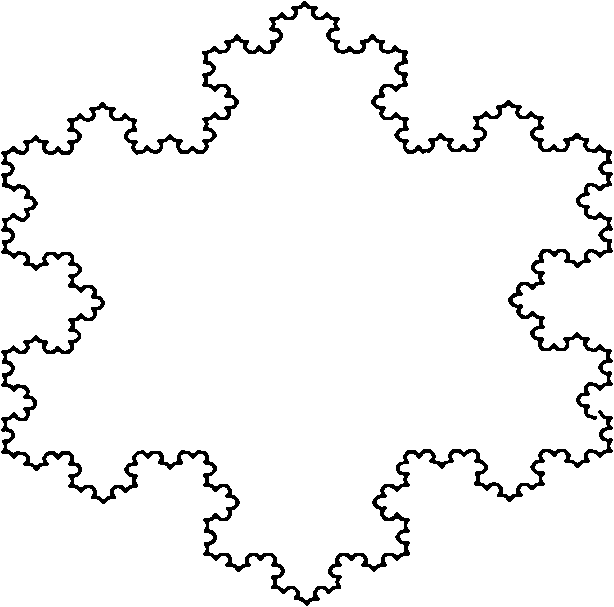
\includegraphics{Images/Img11.png}
    \bigskip
    \caption{The von Koch snowflake.}
    \label{fig:ch5_4.1}
\end{figure}

Brownian motion does not hit points, so it does not hit any of the corners. Yet the Hausdorff dimension of the boundary is larger than $1$, and ``most'' of the boundary points are not hit. The support of harmonic measure, i.e., the smallest closed set whose complement has measure $0$, is actually all of $\partial D$. We are interested in the essential support: a set on which $\omega^{x_0}$ is concentrated.

\mpagebreak

The construction of Lebesgue measure on the line starts out by defining
\begin{align*}
    m(A) = \inf\Big\{\sum_j |I_j| &: I_j~\text{is a countable collection of intervals} \\
    &\qquad\!\text{whose union contains}~A\Big\},
\end{align*}
where $|I_j|$ is just the length of $I_j$. Similarly we start out defining the Le\-besgue measure of $A \subseteq \R^2$ by replacing $I_j$ in the above by balls or squares.

If $\varphi(t)$ is a continuous and increasing function with $\varphi(0) = 0$, define
\begin{align}\label{eq:ch5_4.17}
    \Lambda_\varphi(A) = &\lim_{\delta\to 0}\inf\Big\{\sum_j \varphi(\diam B_j) : B_j~\text{is a collection of balls,} \\
    &\text{each with radius less than}~\delta\text{, whose union contains}~A\Big\}. \notag
\end{align}
$\Lambda_\varphi(A)$ is called the Hausdorff measure of $A$ with respect to the measure function $\varphi$. Except for the restriction that the radii must be less than $\delta$ and the taking of the limit as $\delta \to 0$, this is entirely analogous to the definition of Lebesgue measure.

When $\varphi_\alpha(t) = t^\alpha$ and $A \subseteq \R^d$, it is easy to see (Exercise \ref{ex:ch5_13}) that $\Lambda_{\varphi_\alpha}(A)$ will be $0$ for all $\alpha$ bigger than some $\alpha_0$, and infinite for all $\alpha$ less than $\alpha_0$. When $\alpha = \alpha_0$, it could be infinite, $0$, or some positive number. The number $\alpha = \inf\{\alpha : \Lambda_{\varphi_\alpha}(A) = 0\}$ is called the Hausdorff dimension of $A$. We will denote the measure $\Lambda_{\varphi_\alpha}$ simply by $\Lambda_\alpha$.

The first theorem we prove is the following.

\index{Makarov's theorems}

\begin{theorem}\label{thm:ch5_4.6}
Suppose $D$ is a simply connected domain other than $\C$. There exists $H \subseteq \partial D$ such that the Hausdorff dimension of $H$ is $1$ and $\omega^{x_0}(\partial D - H) = 0$.
\end{theorem}

Thus $\omega^{x_0}$ is concentrated on a set of Hausdorff dimension\index{Hausdorff dimension|)} at most $1$.

Let us say that a subset $A$ of $D$ is a dominating subset\index{Dominating subset} of $D$ if
\[
    \|f\|_\infty = \sup_{z\in A}|f(z)|
\]
for every $f$ that is analytic and bounded in $D$. If almost every boundary point $e^{\im\theta}$ of $\partial\D$ is such that $[\D - B(0,r)] \cap A \cap C_\theta \neq \emptyset$ for all $r$ close to $1$, then $A$ is a dominating subset for $\D$ (Exercise \ref{ex:ch5_14}). If $A$ is a dominating subset of $\D$, then $f(A)$ is a dominating subset of $f(\D)$ (Exercise \ref{ex:ch5_14}).

Let $f$ be a one to one analytic function mapping $\D$ to $D$.

\begin{lemma}\label{lem:ch5_4.7}
Let $\epsilon > 0$. There exists a dominating subset $\widetilde{A}$ of $D$ such that
\[
    \sum_{z\in\widetilde{A}}[\dist(z,\partial D)]^{1+\epsilon} < \infty.
\]
\end{lemma}

\begin{proof}
First, we assert that for almost every $\theta \in [0,2\pi)$,
\begin{equation}\label{eq:ch5_4.18}
    \liminf_{z\in C_\theta,z\to e^{\im\theta}} |f'(z)|(1-|z|)^{\epsilon/(1+\epsilon)} = 0.
\end{equation}
For if not, $\lim_{z\in C_\theta,z\to e^{\im\theta}} |f'(z)| = \infty$ on a set of positive measure. By The\-orem \ref{thm:ch5_3.4}(b), $f'$ is identically infinite, a contradiction.

Let $\eta > 0$. For each $\theta$ not in the null set, there exists $z_\theta \in C_\theta$ such that $1-|z_\theta| < \eta$ and $|f'(z_\theta)| \leq \eta(1-|z|)^{-\epsilon/(1+\epsilon)}$. Let $L_\theta$ be a subarc of $\partial\D$, centered at $e^{\im\theta}$, with length $1-|z_\theta|$. By Corollary \ref{cor:ch5_4.5}, we can find a countable subcollection of the set of arcs $\{L_\theta\}$ such that $\sum_j(1-|z_{\theta_j}|) < \infty$ and $\partial\D - \cup_j L_{\theta_j}$ has $0$ Lebesgue measure.

Let $A_\eta = \{f(z_{\theta_j})\}$. By Corollary \ref{cor:ch5_2.6},
\[
    \dist(f(z),\partial D) \leq c|f'(z)|(1-|z|).
\]
Hence
\begin{align*}
    [\dist(f(z_{\theta_j}),\partial D)]^{1+\epsilon} &\leq c\big[\eta(1-|z_{\theta_j}|)^{-\epsilon/(1+\epsilon)}(1-|z_{\theta_j}|)\big]^{1+\epsilon} \\
    &= c\eta^{1+\epsilon}(1-|z_{\theta_j}|).
\end{align*}
Therefore
\[
    \sum_j[\dist(f(z_{\theta_j}),\partial D)]^{1+\epsilon} \leq c\eta^{1+\epsilon}.
\]

Let $\widetilde{A} = \cup_{k>0}A_{2^{-k}}$. By Exercise \ref{ex:ch5_14}, $A$ is a dominating subset for $D$.
\end{proof}

\begin{proof}[Proof of Theorem \ref{thm:ch5_4.6}]
For each $z \in \widetilde{A}$, let $E_z = \partial D \cap B(z,2\dist(z,\partial D))$. Since $D$ is simply connected, by the proof of Proposition \chapref[II]{prop:ch2_1.14}, $\P^z(Z_{\tau_D} \in E_z) \geq c > 0$. Let $E = \cup_{z\in\widetilde{A}}E_z$.

We claim $\omega^{z_0}(E) = 1$. If not, there exists $F \subseteq \partial D-E$ with $\omega^{z_0}(F) > 0$. Let $h(z) = \P^z(Z_{\tau_D} \in F)$, let $\widetilde{h}$ be the conjugate harmonic function of $h$, and let $f = e^{h+\im\widetilde{h}}$. Then $\|f\|_\infty = e^{\|h\|_\infty}$, and by taking a suitable sequence $z \in D$ converging to a point in $F$, $\|h\|_\infty = 1$. If $z \in \widetilde{A}$, $|f(z)| = e^{h(z)}$, and $h(z) \leq 1-c$, so $|f(z)| \leq e^{1-c}$. This contradicts the fact that $\widetilde{A}$ is a dominating subset. Therefore $\omega^{z_0}(E) = 1$.

Label the points of $\widetilde{A}$ as $z_1,z_2,\ldots$, and for each $m$, let $\widetilde{A}_m = \{z_{k_m},z_{k_m+1},\ldots\}$, where $k_m$ is chosen large so that
\[
    \Big[\sum_{j=k_m}^\infty \dist(z_j,\partial D)\Big]^{1+\epsilon} < 2^{-m}
\]
and $\dist(z_j,\partial D) < 2^{-m}$ if $j \geq k_m$. Let $E_m = \cup_{z\in\widetilde{A}_m}E_z$. Then $\widetilde{A}_m$ is still a dominating subset of $D$, and so $\omega^{z_0}(E_m) = 1$. If $G_\epsilon = \cap_m E_m$, then $\omega^{z_0}(G_\epsilon) = 1$, $G_\epsilon \subseteq E_m$ for all $m$, and $\{B(z_j,2\dist(z_j,\partial D)); z_j \in \widetilde{A}_m\}$ is a cover of $G_\epsilon$ by balls with
\mpagebreak
\[
    \sum_{z_j\in\widetilde{A}_m} (\diam B(z_j,2\dist(z_j,\partial D)))^{1+\epsilon} \leq 2^{1+\epsilon}2^{-m}.
\]
Hence $\Lambda_{1+\epsilon}(G_\epsilon) = 0$. Finally, let $H = \cap_{\ell>0}G_{2^{-\ell}}$. Then $\omega^{z_0}(H) = 1$ and the dimension of $H$ is less than or equal to $1$.
\end{proof}

We now present the result that harmonic measure cannot be concentrated on a set of Hausdorff dimension strictly less than $1$. We suppose $f$ is one to one and continuous on $\D$ and analytic in $\D$.

\begin{lemma}\label{lem:ch5_4.8}
Let $\epsilon > 0$, $\delta \in (0,\epsilon)$, $r \in [1/2,1)$, and $A \subseteq \partial\D$. If $\diam f(A) \leq \epsilon$,
\begin{equation}\label{eq:ch5_4.19}
    |f(rz) - f(z)| \leq \epsilon, \qquad z \in A,
\end{equation}
and
\begin{equation}\label{eq:ch5_4.20}
    (1-r)|f'(rz)| \geq \delta, \qquad z \in A,
\end{equation}
then there exists $c > 2$ such that $A$ can be covered by at most $c(\epsilon/\delta)^2$ sets of diameter $1-r$.
\end{lemma}

\begin{proof}
Consider a grid of squares of mesh size $b\delta$, $b$ to be chosen later. Let $Q_k$ be the squares that contain points of $f(rA)$. Since $\diam f(A) \leq \epsilon$, \eqref{eq:ch5_4.19} implies $\diam f(rA) \leq 3\epsilon$. If $m$ is the number of squares, then
\[
    (b\delta)^2m = |Q_1 \cup \cdots \cup Q_m| \leq c\epsilon^2.
\]
Thus it suffices to show that $A_k = \{z \in A : f(rz) \in Q_k\}$ has diameter less than $1-r$ if $b$ is chosen appropriately.

Suppose $z_1,z_2 \in A_k$ with $|z_1 - z_2| > 1-r$. Then $|rz_1 - rz_2| > r(1-r)$. By Exercise \ref{ex:ch5_15} and \eqref{eq:ch5_4.20},
\begin{equation}\label{eq:ch5_4.21}
    \delta < (1-r^2)|f'(rz_1)| \leq c|f(rz_1) - f(rz_2)| \leq c_1b\delta,
\end{equation}
since $f(rz_1),f(rz_2) \in Q_k$. This is a contradiction if we choose $b = 1/2c_1$.
\end{proof}

\index{Makarov's theorems}

\begin{theorem}\label{thm:ch5_4.9}
Suppose $f$ is one to one and continuous on $\overline{\D}$ and analytic in $\D$. Let $D = f(\D)$. Suppose $\alpha < 1$, $C \subseteq \partial\D$, and $|C| > 0$. Then $\Lambda_\alpha(f(C)) > 0$.
\end{theorem}

\begin{proof}
Let
\begin{equation}\label{eq:ch5_4.22}
    \psi(r) = 2\beta\Big(\log(1/(1-r))\log\log\log(1/(1-r))\Big)^{1/2},
\end{equation}
where $\beta$ is the constant given in Theorem \ref{thm:ch5_3.10}. Since $\log f'$ is a Bloch function, there exist $r_0$ and $A \subseteq C$ such that $|A| > 0$ and
\mpagebreak
\[
    -\psi(r) \leq \log |f'(rz)| \leq \psi(r)
\]
if $z \in A$ and $r \in [r_0,1)$.

Hence
\[
    |f(z) - f(rz)| \leq \int_r^1 |f'(sz)|ds \leq \int_r^1 e^{\psi(s)}ds,
\]
$f(z)$ existing since the integral is finite.

We have the inequality
\[
    \int_r^1 e^{\psi(s)}ds \leq 2(1-r)e^{\psi(r)}
\]
if $r$ is close to $1$. To see this, $g(r) = \int_r^1 e^{\psi(s)}ds - 2(1-r)e^{\psi(r)}$ has $g'(r) > 0$ for $r$ close to $1$ and $\lim_{r\to 1-} g(r) = 0$.

Hence, increasing $r_0$ if necessary,
\[
    |f(z) - f(rz)| \leq 2(1-r)e^{\psi(r)},
\]
if $r \in [r_0,1)$, $z \in A$. Let $\{B_k\}$ be any collection of sets that are the intersection of open balls with $\partial D$ such that $\cup_k B_k$ contains $f(A)$, and let $A_k = \{z \in A : f(z) \in B_k\}$. Let $\epsilon_k = \diam B_k$, define $r_k$ so that $\epsilon_k = 2(1-r_k)e^{\psi(r_k)}$, and let $\delta_k = (1-r_k)e^{-\psi(r_k)}$. By Lemma \ref{lem:ch5_4.8}, $A_k$ can be covered by at most $c(\epsilon_k/\delta_k)^2$ sets of diameter $1-r_k$. So
\begin{align*}
    |A| &\leq \sum_k |A_k| \leq c\sum_k(\epsilon_k/\delta_k)^2(1-r_k) \\
    &= c\sum_k(1-r_k)e^{4\psi(r_k)} \leq c\sum_k\varphi_\alpha(\epsilon_k).
\end{align*}
Hence $\Lambda_\alpha(f(A)) \geq |A|/c > 0$.
\end{proof}

\begin{corollary}\label{cor:ch5_4.10}
Suppose $B \subseteq \partial D$ has positive harmonic measure. Then the Hausdorff dimension of $B$ is at least $1$.
\end{corollary}

\begin{proof}
By L\'evy's theorem (Theorem \ref{thm:ch5_1.2}), $C = f^{-1}(B)$ has positive harmonic measure in $\D$, hence $|C| > 0$. Theorem \ref{thm:ch5_4.9} says that $\Lambda_\alpha(B) = \Lambda_\alpha(f(C)) > 0$ for all $\alpha < 1$, which implies that $B$ has Hausdorff dimension at least $1$.
\end{proof}

Both for the lower and upper bounds stronger statements can be made. Rather than bounds on Hausdorff dimensions, one can even describe which Hausdorff measure functions give $0$ or infinite mass to the set on which harmonic measure is concentrated (see \cite{Makarov1985} or \cite{Pommerenke1992}; see also \cite{Wolff1993}).

If $D$ is multiply connected, the upper bound on the Hausdorff dimension still holds; see \cite{JonesWolff1988}. There is no lower bound in this case; given any $\alpha < 1$, sets of Hausdorff dimension $\alpha$ can be shown to be hit by two-dimensional Brownian motion (Exercise \ref{ex:ch5_27}), and so if $D$ is the complement of one of these sets, the support of harmonic measure will have Hausdorff dimension $\alpha$.

When $d > 2$ it is not true that the support of harmonic measure lies in a set of Hausdorff dimension of at most $d-1$ (see \cite{Wolff1987}). However, there exists $\epsilon$ depending only on $d$ such that the Hausdorff dimension of the support of harmonic measure is at most $d-\epsilon$ (see \cite{Bourgain1987}).

\section{The angular derivative problem}\label{ch5_sec5}

\subsecbkm{ch5_sec5.1}{Angular derivatives}

In this section we give an introduction to the angular derivative problem. We have seen in Theorem \ref{thm:ch5_1.14} that any simply connected domain can be mapped one to one onto the unit disk. We are now interested in: when is this mapping smooth? When does it have a derivative? More precisely, if $f : \D \to D$ is one to one and analytic, what are geometric conditions on $D$ such that $f'$ has a nontangential limit at a given boundary point? That is, does $\lim_{z\in C_\theta,z\to e^{\im\theta}} f'(z)$ exist and is it nonzero? This limit, when it exists, is called the angular derivative\index{Angular derivative}.

Sometimes instead of the above, one sees the definition of angular derivative as
\begin{equation}\label{eq:ch5_5.1}
    \lim_{z\in C_\theta,z\to e^{\im\theta}} \frac{f(z) - f(e^{\im\theta})}{z - e^{\im\theta}} = a,
\end{equation}
where $a \neq \infty$ and $f(e^{\im\theta})$ is the radial limit of $f$. The radial limit of $f$ at $e^{\im\theta}$ is $\lim_{r\to 1} f(re^{\im\theta})$.

These definitions are equivalent, since we have the following.

\begin{proposition}\label{prop:ch5_5.1}
$f$ has angular derivative $a$ at $e^{\im\theta}$ if and only if $f$ has a radial limit at $e^{\im\theta}$ and
\[
    \lim_{z\in C_\theta,z\to e^{\im\theta}} \frac{f(z) - f(e^{\im\theta})}{z - e^{\im\theta}} = a.
\]
\end{proposition}

\begin{proof}
Suppose $f$ has an angular derivative at $e^{\im\theta}$. The radial limit exists since $f(re^{\im\theta}) = e^{\im\theta}\int_0^r f'(se^{\im\theta})ds$ converges as $r \to 1$. Since $z(1-t)+te^{\im\theta} \in C_\theta$ if $t \in (0,1)$ and $z \in C_\theta$ by the convexity of $C_\theta$, then
\[
    \frac{f(e^{\im\theta}) - f(z)}{e^{\im\theta} - z} = \int_0^1 f'(z + (e^{\im\theta}-z)t)dt \to a
\]
as $z \to e^{\im\theta}$ with $z \in C_\theta$.

To prove the converse, suppose $z_n \in C_\theta$, $z_n \to e^{\im\theta}$. Let
\[
    g_n(s) = \frac{1}{e^{\im\theta} - z_n}[f(z_n + (e^{\im\theta} - z_n)s) - f(e^{\im\theta})].
\]
As $n \to \infty$, $g_n(s) \to a(s-1)$ uniformly over $|s| \leq 1/2$. Hence $g'_n(0) \to a$. However, $g'_n(0) = f'(z_n)$.
\end{proof}

Since the disk $\D$ and the half-space $H = \{\Im z > 0\}$ are mapped into each other by a smooth mapping, we may as well work with mappings from $H$ into $\D$. We will investigate the existence of the angular derivative at the boundary point 0 and we assume $f: H \to \D$ is such that $f(0) = 0$.

Set
\begin{equation}\label{eq:ch5_5.2}
    V_0 = \{x + \im y \in H : |x| < y\}.
\end{equation}
We want to know when $\lim_{z \in V_0,z \to 0} f(z)/z$ exists and is a finite positive real number. We will make some nontrivial simplifying assumptions in the remainder of the section:
\begin{obs}\label{obs:ch5_5.3}
    \textit{$\partial D$ has $\partial H$ as a tangent line at $0$, $V_0$ is contained in $D$, $-V_0$ is contained in $D^c$, and $f$ has a continuous extension to $\overline{H}$.}
\end{obs}

Let us make some comments about these assumptions. Saying $\partial D$ has a tangent at $0$ means that
\[
    \lim_{z \in \partial \D,z \to 0-} \arg f(z) = \pi \qquad \text{and} \qquad \lim_{z \in \partial \D,z \to 0+} \arg f(z) = 0,
\]
where $\arg w$ is the imaginary part of $\log w$. A necessary and sufficient condition for $f$ to have an extension to $\overline{H}$ is that $\partial D$ be a Jordan curve\index{Jordan curve} (see \cite{Pommerenke1975} for a proof); here we make this our assumption. Finally, there exist $f$ that have angular derivatives at $0$ but for which $\partial D$ does not have a tangent (Exercise \ref{ex:ch5_17}).

\begin{proposition}\label{prop:ch5_5.2}
If $D$ has a tangent at $0$, then $\lim_{z \in H,z \to 0} \arg(f(z)/z)$ exists.
\end{proposition}

\begin{proof}
Let $w(z) = \arg(f(z)/z) = \arg f(z) - \arg z$. The assumption that $D$ has a tangent at $0$ implies that $w$ restricted to $\partial H$ is continuous at $0$. Since $f$ has a continuous extension to $\partial H$, $w$ restricted to $\partial H$ is continuous away from $0$. Since $V_0 \subseteq D$ and $-V_0 \subseteq D^c$, $w$ is bounded. Since $w$ is harmonic in $H$, it follows by Theorem \chapref[II]{thm:ch2_1.15} that $w(z)$ is continuous at $0$ over $z \in H$.
\end{proof}

Since we are assuming $D$ has a tangent at 0, we need to look at the nontangential limit of $|f(z)|/|z|$. It is actually enough to look at the radial limit\index{Radial limit|(}. Let
\begin{equation}\label{eq:ch5_5.4}
    I = \{\im y : y > 0\}.
\end{equation}

\begin{proposition}\label{prop:ch5_5.3}
Suppose
\[
    \lim_{z \in I,z \to 0} |f(z)/z| = a \in (0,\infty) \qquad \text{and} \qquad \arg_{z \in H,z \to 0} \arg(f(z)/z) = 0.
\]
Then $\lim_{z \in V_0,z \to 0} |f(z)/z| = a$.
\end{proposition}

\begin{proof}
Let $V_1 = \{x + \im y : |x| < 2y\}$. Let $\epsilon > 0$. Since $f$ is one to one and nonzero in $H$, then $g(z) = \log(f(z)/z)$ is a single-valued analytic function in $H$. Since $\Im g(z) \to 0$ as $z \to 0$, then $|\Im g(z)| < \epsilon$ for $z = x + \im y \in V_1$ provided $y$ is sufficiently small. By Corollary \chapref[II]{cor:ch2_1.4}, $|\nabla\Im g(x + iy)| \leq c\epsilon/y$ if $x + iy \in V_0$ and $y$ is sufficiently small. Since $|\nabla\Re g| = |\nabla\Im g|$ by the Cauchy-Riemann equations,
\begin{align*}
    |\Re g(x + \im y) - \log a| &\leq |\Re g(\im y) - \log a| + |x|c\epsilon/y \\
    &\leq |\Re g(\im y) - \log a| + c\epsilon
\end{align*}
if $x+\im y \in V_0$ and $y$ is sufficiently small. Since $\epsilon$ is arbitrary and $\Re g(\im y) \to \log a$ as $y \to 0$, the result follows.
\end{proof}

\index{Radial limit|)}

For a generalization to the case where $\arg(f(z)/z)$ does not tend to $0$, see \cite{Pommerenke1975}.

We next convert the question of radial limits of $|f(z)/z|$ to one about the normal derivative\index{Normal derivative} of the Green function.

\begin{proposition}\label{prop:ch5_5.4}
Suppose $D$ is as above. Fix $w_0 \in D$. Then $D$ has an angular derivative at $0$ if and only if the normal derivative of $g_D(y,w_0)$ at $0$ is positive and finite.
\end{proposition}

\begin{proof}
Let $\Gamma = f^{-1}(I)$, where $I$ is defined in \eqref{eq:ch5_5.4}. A very similar argument to the proof of Proposition \ref{prop:ch5_5.3} shows that
\begin{equation}\label{eq:ch5_5.5}
    \lim_{z \in V_0,z \to 0}|f(z)|/|z| = \lim_{z \in \Gamma,z \to 0}|f(z)|/|z|.
\end{equation}
Since $f'(0)$ is real (because $\arg f'(0) = 0$) and positive, $\lim_{z \in \Gamma,z \to 0} \Im z/|z| \allowbreak = 1$. It is easy, by Proposition \chapref[II]{prop:ch2_3.8}, to see that $\lim_{z \to 0,z \in H} g_H(z,y_0)/\Im z$ exists and is positive for every $y_0 \in H$. So the expression in \eqref{eq:ch5_5.5} is equal to
\begin{align*}
    \lim_{z \in \Gamma,z \to 0} c|f(z)|/g_H&(z,f^{-1}(w_0)) \\
    &= \lim_{w \in I,w \to 0} c|f(f^{-1}(w))|/g_D(f^{-1}(w),f^{-1}(w_0)) \\
    &= \lim_{w \in I,w \to 0} c|w|/g_D(w,w_0),
\end{align*}
since $g_H(z,w) = g_D(f(z),f(w))$ by Exercise \ref{ex:ch5_18}.
\end{proof}

\subsecbkm{ch5_sec5.2}{Ratios of harmonic functions}
\index{Ratios of harmonic functions|(}

The following proposition will allow us to prove the existence of a normal derivative by proving upper and lower bounds on $g_D(\im y,w_0)/y$, $y > 0$. See \cite{Bass1994} for generalizations.

\begin{proposition}\label{prop:ch5_5.5}
Suppose $d = 2$, $N > 1$, $D$ is the intersection of the region above the graph of a Lipschitz function with $B(0,N)$, $0 \in \partial D$, and $w_0 \in D$. Suppose $u$ is positive and harmonic in $D$. Then
\begin{equation}\label{eq:ch5_5.6}
    \lim_{y\downarrow 0} u(\im y)/g_D(\im y,w_0) = \liminf_{z \in D,z \to 0} u(z)/g_D(z,w_0).
\end{equation}
\end{proposition}

\begin{proof}
Let $z, z_1$ be points in $D \cap B(0,|w_0|/2)$. By Exercise \ref{ex:ch5_21}, there exists $c_1$ such that
\[
    \frac{g_D(z,w_0)g_D(w_0,z_1)}{g_D(z,z_1)} \leq c[1 + \log^+(1/|z - w_0|) + \log^+(1/|z_1 - w_0|)] \leq c_1.
\]
If we let $z_1 \to 0$ in $D$, we see that
\begin{equation}\label{eq:ch5_5.7}
    g_D(z,w_0)/M(z,0) \leq c_1,
\end{equation}
where $M(z,0)$ is the Martin kernel with pole at $0$. As usual, we abbreviate $\P^w_{M(\cdot,0)}$ by $\P^w_0$.

Let $\ell = \liminf_{z \in D,z \to 0} u(z)/g_D(z,w_0)$. Our result is trivial if $\ell = \infty$, so let us suppose $\ell < \infty$. Let $\epsilon > 0$ and
\[
    A = \{z \in D \cap B(0,|w_0|/2) : u(z) - (\ell+\epsilon)g_D(z,w_0) > 0\}.
\]
Since $g_D(\cdot,w_0)$ and $u$ are harmonic in $D \cap B(0,|w_0|/2)$, $A$ is open. Let
\begin{equation}\label{eq:ch5_5.8}
    L_t = \big[u(Z_t) - (\ell + \epsilon)g_D(Z_t,w_0)\big]/M(Z_t,0).
\end{equation}
It is easy to see that $L_t$ is a martingale with respect to $\P^w_0$ for each $w \in D$, and by \eqref{eq:ch5_5.7}, $L_t$ is bounded below by $-c_1(\ell + \epsilon)$ when $Z_t$ is in $D \cap B(0,|w_0|/2)$.

If we use the definition of $\ell$ to choose $w$ close to $0$ with $u(w)/g_D(w,w_0) \allowbreak < \ell + \epsilon/2$, we see by the optional stopping theorem (Theorem \chapref[I]{thm:ch1_4.4}) and dominated convergence that
\[
    \E^w_0 L_{T_A \wedge \tau_D} < -\frac{\epsilon g_D(w,w_0)}{2M(w,0)}.
\]
So $\P^w_0(T_A < \tau_D) < 1$. By the zero-one law (Proposition \chapref[III]{prop:ch3_2.7}),
\[
    \P^w_0(\limsup_{t \to \tau_D} L_t > 0) = 0,
\]
or
\mpagebreak
\[
    \P^w_0(\limsup_{t \to \tau_D} u(Z_t)/g_D(Z_t,w_0) > \ell + \epsilon) = 0.
\]
Clearly, $\liminf_{t \to \tau_D} u(Z_t)/g_D(Z_t,w_0) \geq \ell$ under $\P_w$, and so the limit of $u(Z_t)/g_D(Z_t,w_0)$ exists and equals $\ell$, $\P^0_w$-a.s.

Let $y_n$ be any sequence tending to $0$ with $u(\im y_n)/g_D(\im y_n,w_0) \to a < \infty$. By the Harnack inequality applied to $g_D(z,w_0)$ and $u(z)$, there exists $c$ such that $|u(z)/g_D(z,w_0)-a| < \epsilon$ if $z \in B(\im y_n,cy_n)$ for some $n$. By the argument of Theorem \chapref[III]{thm:ch3_4.3} or Proposition \ref{prop:ch5_3.1}, we must have $\ell = a$. A similar argument holds for sequences $y_n$ tending to $0$ with $u(\im y_n)/g_D(\im y_n,w_0) \to \infty$. The proposition follows.
\end{proof}

\index{Ratios of harmonic functions|)}

\subsecbkm{ch5_sec5.3}{Domains contained in a half-space}

We will look at the cases when $D \subseteq H$, $D \supseteq H$, and more general domains separately. Let us here suppose $D \subseteq H$ and let us further suppose that

\begin{obs}\label{obs:ch5_5.9}
    \textit{$D$ is the region above the graph of a Lipschitz function $F$ that is bounded by $1$ and has Lipschitz constant at most $1$.}
\end{obs}

For domains satisfying \eqref{obs:ch5_5.9} we can give a complete answer to the angular derivative problem.

\begin{theorem}\label{thm:ch5_5.6}
Suppose $D$ satisfies \eqref{obs:ch5_5.3} and \eqref{obs:ch5_5.9}. Let $w_0 \in D$. $g_D(\cdot,w_0)$ has a normal derivative at $0$ (and hence the angular derivative exists) if and only if $\int_{-\infty}^{\infty} F(x)/x^2dx < \infty$.
\end{theorem}

To begin the proof of Theorem \ref{thm:ch5_5.6}, we first want to reduce to the case where $F(x)$ is $0$ if $|x| \geq 8$. Let
\[
    F_1(x) = \begin{cases}
        0 & \text{if}~|x| \geq 8,\\
        1 & \text{if}~|x| \leq 7,\\
        8-|x| & \text{if}~7 < |x| < 8
    \end{cases}
\]
and let $D_1$ be the union of $D$ and the region above the graph of $F_1$. $D_1$ still satisfies the conditions \eqref{obs:ch5_5.3} and \eqref{obs:ch5_5.9}. By the boundary Harnack principle in $D$ with the harmonic functions $u = g_{D_1}(\cdot,w_0)$ and $v = g_D(\cdot,w_0)$, we see $g_D(\cdot,w_0)/g_{D_1}(\cdot,w_0)$ is bounded above and below by positive constants in a neighborhood of $0$. So the normal derivative of $g_D$ at $0$ will be finite and positive if and only if the normal derivative of $g_{D_1}$ is positive and finite at $0$. Hence without loss of generality we may assume that $F(x) = 0$ if $|x| \geq 8$.

\begin{proof}[Proof of Theorem \ref{thm:ch5_5.6}]
Since $D \subseteq H$, then $g_D(z,w) \leq g_H(z,w)$ for all $z,w \in \allowbreak D$. An easy calculation with Proposition \chapref[II]{prop:ch2_3.8} shows that $g_H(\im y,w_0)/y$ converges to a finite positive limit as $y \downarrow 0$ for each $w_0$, hence $\lim_{y \downarrow 0} g_D(\im y,w_0)/y \allowbreak < \infty$. By Proposition \ref{prop:ch5_5.5} in $D \cap B(0,1)$ with $u(z) = \Im z$, it suffices to show $\liminf_{y \downarrow 0} g_D(\im y,w_0)/y > 0$.

\mpagebreak

Let $U = \{x + \im y : y = 10\}$. In $D \cap B(0,1)$, $g_D(z,w_0)$ and $\P^z(T_U < \tau_D)$ are both positive harmonic functions that vanish on $\partial D$. So by the boundary Harnack principle these two functions are comparable near $0$. It therefore suffices to show
\begin{equation}\label{eq:ch5_5.10}
    \frac{\P^{\im y}(T_U < \tau_D)}{y} \geq c
\end{equation}
for some positive constant $c$ and for $y$ close to $0$.

Let $h(x + \im y) = y$. This is harmonic and $(\P^z_h, X_t)$ is Brownian motion in $H$ conditioned to hit $U$ before $\partial H$.
\[
    \P^{\im y}(T_U < \tau_D)/y = c\P^{\im y}_h(T_U < \tau_D).
\]
Now Brownian motion in $H$ $h$-path transformed by this particular $h$ still has independent components. $X_t$ is still a Brownian motion and (see Exercise \ref{ex:ch5_19}) $Y_t$ has the same law as the modulus of a three-dimensional Brownian motion. Let
\[
    A = \big\{(x^1,x^2,x^3,x^4) : \big((x^2)^2 + (x^3)^2 + (x^4)^2\big)^{1/2} \geq F(x^1)\big\}.
\]
Let $W_t$ be a four-dimensional Brownian motion. What we look at is $\P^0(T_A < \tau_V)$, where $B(0,10)$ is the ball of radius 10 in $\R^3$, $V = \R \times B(0,10)$, and $T_A$ and $\tau_V$ are defined relative to $W_t$.

Let $A_k = \{x \in A : 2^{-(k+1)} < |x| \leq 2^{-k}\}$. By Lemma \ref{lem:ch5_5.7}, $\int_{-8}^8 F(x)/x^2dx = \infty$ if and only if $\sum 2^{2k}C(A_k) = \infty$, where $C(A_k)$ is the capacity (relative to $W_t$) of $A_k$. If $\sum 2^{2k}C(A_k) = \infty$, then by Wiener's test (Theorem \chapref[II]{thm:ch2_5.15}), $0$ is regular for $A$, hence $\P^0(T_A < \tau_V) = 1$. In this case $\P^y(T_A > \tau_V) \to 0$ as $|y| \to 0$, and so the normal derivative of $g_D$ is $0$ at $0$. On the other hand, $\sum 2^{2k}C(A_k) < \infty$ implies $\P^0(T_A = 0) = 0$. Then $\P^0(T_A > \tau_V) > 0$. Therefore (Exercise \ref{ex:ch5_20}) $\P^y(T_A > \tau_V)$ is bounded away from $0$ for $y$ in the intersection of $I$ with a neighborhood of $0$, which implies \eqref{eq:ch5_5.10}.
\end{proof}

\begin{lemma}\label{lem:ch5_5.7}
$\sum 2^{2k}C(A_k) = \infty$ if and only if $\int_{-8}^8 F(x)/x^2dx = \infty$.
\end{lemma}

\begin{proof}
Let $I$ be the interval $[0,1]$ and let
\[
    B = \big\{(x^1,x^2,x^3,x^4) : x^1 \in I, \big((x^2)^2 + (x^3)^2 + (x^4)^2\big)^{1/2} \leq F(x^1)\big\}.
\]
We show there exist constants $c_1$ and $c_2$ such that
\begin{equation}\label{eq:ch5_5.11}
c_1 \int_I F(x)dx \leq C(B) \leq c_2 \int_I F(x)dx.
\end{equation}
The lemma will follow by scaling and summing over the collections of intervals $(2^{-(k+1)},2^{-k}]$ and $[-2^{-k},2^{-(k+1)})$.

Let us form a collection of disjoint intervals. Divide $I$ into two equal subintervals. If there exists $x \in [0,1/2)$ such that $F(x) \geq 1$, we select $[0,1/2)$ as one of our intervals; otherwise we divide $[0,1/2)$ into two equal subintervals and continue. We also perform this procedure on $[1/2,1]$. We select an interval $J_i$ if there exists a point $x$ in it for which $F(x) \geq 2|I_i|$. More precisely, an interval $J=[k/2^m,(k+1)/2^m)$ is one of our intervals if there exists $x\in J$ with $F(x)\ge 2|J|$ and $J$ is not contained in any larger dyadic interval $J'$ for which there exists $y \in J'$ with $F(y) \geq 2|J'|$.

Since $F$ is Lipschitz with Lipschitz constant at most $1$, $F \geq |J_i|$ on the interval $J_i$ in our sequence. Since $J_i$ is not contained in any larger interval in the sequence, $F \leq 2|J_i|$ on $J_i$. Note $F = 0$, a.e., on $I - \cup_i J_i$.

Let $B_i = B \cap \{(x^1,x^2,x^3,x^4) : x^1 \in J_i\}$. By the estimate of Proposition \chapref[II]{prop:ch2_5.16} for the capacity of a cylinder, there exists $c$ such that
\begin{equation}\label{eq:ch5_5.12}
    c^{-1}|J_i|^2 \leq C(B_i) \leq c|J_i|^2.
\end{equation}
Therefore
\begin{align*}
    C(B) &\leq \sum_i C(B_i) \leq c\sum_i |J_i|^2 \\
    &\leq c\sum_i \int_{J_i} F(x)dx = c \int_I F(x)dx.
\end{align*}

If $J_i = [k/2^m,(k+1)/2^m)$, let $\widetilde{J}_i = [(k-1/2-\epsilon)/2^m,(k+1/2+\epsilon)/2^m]$, where $\epsilon$ will be chosen later and let $\widetilde{B}_i = B \cap \{(x^1,x^2,x^3,x^4): x^1 \in \widetilde{J}_i\}$. By Propositions \chapref[II]{prop:ch2_5.16} and \chapref[II]{prop:ch2_5.11}, there exists $c$ such that
\begin{equation}\label{eq:ch5_5.13}
    |J_i|^2 \leq cC(\widetilde{B}_i).
\end{equation}

By Proposition \chapref[II]{prop:ch2_5.8},
\begin{equation}\label{eq:ch5_5.14}
    C(B) = c \int \P^y(T_B < \infty)\sigma(dy),
\end{equation}
where $\sigma$ is normalized surface measure on $\partial B(0,6)$ and $T_B$ is defined in terms of $W_t$, a four-dimensional Brownian motion. If $|y| = 6$,

\tweakpage{0.5}

\begin{equation}\label{eq:ch5_5.15}
\P^y(T_B < \infty) \geq \sum_i \P^y(T_{\widetilde{B}_i} < \infty) - \sum_{i\neq j} \P^y(T_{\widetilde{B}_i} < \infty, T_{\widetilde{B}_j} < \infty).
\end{equation}
As in the proof of Theorem \chapref[II]{thm:ch2_5.15},
\begin{align}\label{eq:ch5_5.16}
    \P^y(T_{\widetilde{B}_i} < \infty, T_{\widetilde{B}_j} < \infty) &\leq \P^y(T_{\widetilde{B}_i} < \infty, T_{\widetilde{B}_j} \circ \theta_{T(\widetilde{B}_i)} < \infty) \\
    &\qquad+ \P^y(T_{\widetilde{B}_j} < \infty, T_{\widetilde{B}_i} \circ \theta_{T(\widetilde{B}_j)} < \infty) \notag
\end{align}
and
\begin{align}\label{eq:ch5_5.17}
    \P^y(T_{\widetilde{B}_i} < \infty,\,&T_{\widetilde{B}_j} \circ \theta_{T(\widetilde{B}_i)} < \infty) \\
    &= \E^y\big[\P^{W_{T(\widetilde{B}_i)}}(T_{\widetilde{B}_j} < \infty); T_{\widetilde{B}_i} < \infty\big]. \notag
\end{align}

\mnewpage

Let $x_i$ be the center of $J_i$ and let $r_{ij} = |x_i - x_j|$. If $w \in \widetilde{B}_i$, then by Proposition \chapref[I]{prop:ch1_5.8}
\begin{equation}\label{eq:ch5_5.18}
    \P^w(T_{\widetilde{B}_j} < \infty) \leq c(\epsilon)|J_j|^2r_{ij}^{-2}
\end{equation}
where $c(\epsilon)$ is a constant that goes to $0$ as $\epsilon \to 0$. Substituting in \eqref{eq:ch5_5.16} and \eqref{eq:ch5_5.17},
\begin{align*}
    \P^y(T_{\widetilde{B}_i} < \infty, T_{\widetilde{B}_j} < \infty) &\leq c(\epsilon)|J_i|^2r_{ij}^{-2}\P^y(T_{\widetilde{B}_i} < \infty) \\
    &\qquad+ c(\epsilon)|J_j|^2r_{ij}^{-2}\P^y(T_{\widetilde{B}_j} < \infty).
\end{align*}
Putting this in \eqref{eq:ch5_5.14} and \eqref{eq:ch5_5.15},
\begin{align}\label{eq:ch5_5.19}
    C(B) &\geq \sum_i C(\widetilde{B}_i) - c(\epsilon)\sum_{i\neq j}\big\{|J_j|^2 r_{ij}^{-2}C(\widetilde{B}_i)+|J_i|^2 r_{ij}^{-2}C(\widetilde{B}_j)\big\} \\
    &\geq\sum_i C(\widetilde{B}_i) - c(\epsilon)\sum_{i\neq j}C(\widetilde{B}_i)C(\widetilde{B}_j)r_{ij}^{-2}, \notag
\end{align}
using \eqref{eq:ch5_5.13}.

If $y \in \widetilde{J}_j$, $|y - x_i| \leq cr_{ij}$. Suppose $|J_j| \leq |J_i|$. By \eqref{eq:ch5_5.12},
\[
    C(\widetilde{B}_j)r_{ij}^{-2} \leq c|J_j|^2r_{ij}^{-2} \leq c|J_j| \int_{\widetilde{J}_j} \frac{dy}{|y - x_i|^2} \leq c|J_i| \int_{\widetilde{J}_j} \frac{dy}{|y - x_i|^2}.
\]
Then
\[
    \sum_{\{j:|J_j|\leq|J_i|,i\neq j\}} C(\widetilde{B}_j)r_{ij}^{-2} \leq c|J_i| \int_{J_i^c} \frac{dy}{|y - x_i|^2} \leq c|J_i||J_i|^{-1} \leq c.
\]
This gives us
\begin{align*}
    c(\epsilon) \sum_{i,j} C(\widetilde{B}_i)C(\widetilde{B}_j)r_{ij}^{-2} &\leq 2c(\epsilon) \sum_{|J_i|\geq|J_j|,i\neq j} C(\widetilde{B}_i)C(\widetilde{B}_j)r_{ij}^{-2} \\
    &\leq c(\epsilon)\sum_i C(\widetilde{B}_i) \leq \frac{1}{2}\sum_i C(\widetilde{B}_i)
\end{align*}
if $\epsilon$ is small enough. Finally, substituting in \eqref{eq:ch5_5.19},
\begin{align*}
    C(B) &\geq \sum_i C(\widetilde{B}_i)-\frac{1}{2}\sum_i C(\widetilde{B}_i) \geq c\sum_i |J_i|^2 \\
    &\geq c\sum_i \int_{J_i} F(x)dx = c\int_I F(x)dx.
\end{align*}
\end{proof}

\subsecbkm{ch5_sec5.4}{Domains containing a half-plane}

Next we turn to the case $D \supseteq H$. Let us suppose $D$ is the region above $-F(x)$, where $F(x)$ is a nonnegative Lipschitz function bounded by $1$ with Lipschitz constant at most $1$ and that $D$ satisfies \eqref{obs:ch5_5.3}. Let $w_0 \in D$. As above, there is no loss of generality in assuming $F(x) = 0$ if $|x| \geq 8$.

\begin{theorem}\label{thm:ch5_5.8}
Suppose $D$ is as above. Then the normal derivative of $g_D(\cdot,w_0)$ at $0$ is positive and finite (and hence the angular derivative exists) if and only if $\int_{-\infty}^{\infty} F(x)/x^2dx < \infty$.
\end{theorem}

We prove this theorem in a number of steps. Let $U = \{x+\im y : y = 10\}$.

\begin{proposition}\label{prop:ch5_5.9}
The normal derivative of $g_D(\cdot,w_0)$ is positive and finite if and only if
\[
    \int_{-8}^8 \frac{\P^x(T_U < \tau_D)}{|x|^2}dx < \infty.
\]
\end{proposition}

\begin{proof}
Since $H \subseteq D$, $g_D(z,w) \geq g_H(z,w)$ for all $z$ and $w$. As in Theorem \ref{thm:ch5_5.6},
\[
    \liminf_{y\downarrow 0} g_D(\im y,w_0)/y \geq \lim_{y\downarrow 0} g_H(\im y,w_0)/y > 0.
\]

We will show
\begin{equation}\label{eq:ch5_5.20}
    \limsup_{y\downarrow 0} g_D(\im y,w_0)/y < \infty.
\end{equation}
Since $g_D(\cdot,w_0)$ is harmonic in $H - \{w_0\}$,
\[
    \frac{g_D(\im y,w_0)}{y} = \frac{1}{y}\int_{\partial H} \frac{1}{\pi} \frac{y}{x^2 + y^2}g_D(x,w_0)dx = \int_{\partial H} \frac{1}{\pi} \frac{g_D(x,w_0)}{x^2 + y^2}dx.
\]
Because this increases as $y \downarrow 0$, convergence along a subsequence $y_n \downarrow 0$ implies the existence of the limit as $y \downarrow 0$.

As in the proof of Theorem \ref{thm:ch5_5.6}, the boundedness of \eqref{eq:ch5_5.20} is equivalent to the boundedness of $\P^{iy}(T_U < \tau_D)/y$ near $0$.
\[
    \P^{\im y}(T_U < \tau_D) = \E^{\im y}[\P^{X_{T(\partial H)}}(T_U < \tau_D)] = \int_{-\infty}^{\infty} P_H(\im y,x)\P^x(T_U < \tau_D)dx,
\]
where $P_H$ is the Poisson kernel for $H$. We have
\[
    P_H(\im y,x) = \frac{y}{\pi(y^2 + x^2)} \leq \frac{cy}{x^2},
\]
so
\[
    \frac{\P^{\im y}(T_U < \tau_D)}{y} \leq c\int_{-\infty}^{\infty} \P^x(T_U < \tau_D)/x^2 dx.
\]
On the other hand,
\mpagebreak
\[
    \frac{\P^{\im y}(T_U < \tau_D)}{y} \to c\int_{-\infty}^{\infty} \P^x(T_U < \tau_D)/x^2 dx
\]
as $y \to 0$ by the monotone convergence theorem.

To complete the proof, we observe that $F(x) = 0$ and so $\P^x(T_U < \tau_D) = 0$ if $|x| \geq 8$. Hence we can replace the integral $\int_{-\infty}^{\infty}$ by the integral $\int_{-8}^8$.
\end{proof}

\begin{lemma}\label{lem:ch5_5.10}
There exists $c$ such that if $x \in \partial H$, then $\P^x(T_U < \tau_D) \geq cF(x)$.
\end{lemma}

\begin{proof}
Let $x \in \partial H$. Since $F$ is Lipschitz with constant at most 1, $Q(x) \subseteq D$, where $Q(x)$ is the rectangle $[x-F(x)/4,x+F(x)/4] \times [-F(x)/4,6F(x)]$. Let $V(x)$ be the upper boundary of $Q(x)$. By scaling and the support theorem, $\P^x(T_{V(x)} < \tau_D) \geq c$. If $y \in V(x)$,
\[
    \P^y(T_U < \tau_D) \geq \P^y(T_U < \tau_{\partial H}) \geq cF(x)
\]
by Proposition \chapref[I]{prop:ch1_4.9}. So by the strong Markov property, $\P^x(T_U < \tau_D) \geq cF(x)$.
\end{proof}

The converse of Lemma \ref{lem:ch5_5.10} is not true and a slightly different argument is needed.

\begin{proof}[Proof of Theorem 5.8]
If $\int_{-8}^8 F(x)/x^2dx = \infty$, then by Lemma \ref{lem:ch5_5.10}, $\int_{-8}^8 \P^x(T_U < \tau_D)/x^2dx = \infty$, and hence the normal derivative of $g_D(\cdot,w_0)$ is infinite by Proposition \ref{prop:ch5_5.9}.

So let us suppose $\int_{-8}^8 F(x)/x^2dx < \infty$. Set $\overline{\mu}(dx) = 1_{[1,2]}(|x|)dx$, a measure on $\partial H$, and let $\overline{R} = D \cap \{x + \im y : 1/2 \leq x \leq 4\}$. We claim
\begin{equation}\label{eq:ch5_5.21}
    \int \P^x(T_U < \tau_{\overline{R}})\overline{\mu}(dx) \leq c \int_{1/2}^4 F(x)dx.
\end{equation}

Let us show how \eqref{eq:ch5_5.21} is used to prove the theorem. Let $\mu(dx) = 1_{[1,2]}(|x|)dx$ and $R = D \cap \{x + iy : 1/2 \leq |x| \leq 4\}$. By symmetry and an addition, \eqref{eq:ch5_5.21} implies that
\[
    \int \P^x(T_U < \tau_R)\mu(dx) \leq c \int_{1/2 \leq |x| \leq 4} F(x)dx.
\]
Let $\mu_k(dx) = 1_{[2^{-k-1},2^{-k+2}]}(|x|)dx$ and $R_k = D \cap \{x + \im y : 2^{-k-1} \leq |x| \leq 2^{-k+2}\}$. By scaling,
\[
    \int \P^x(T_U < \tau_{R_k})\frac{\mu_k(dx)}{\mu_k(\R)} \leq c2^k \int_{2^{-k-1} \leq |x| \leq 2^{-k+2}} F(x)dx.
\]
Note $\mu_k(\R) = c2^{-k}$. Since $x^{-2}$ is comparable to $2^{2k}$ for $|x| \in [2^{-k-1},2^{-k+2}]$, taking the sum over $k$ leads to
\mpagebreak
\begin{align*}
    \int_{-8}^8 \P^x(T_U < \tau_D)/x^2dx &\leq c\sum_k 2^{2k} \int \P^x(T_U < \tau_D)\mu_k(dx) \\
    &\leq c\sum_{k} 2^k \int_{\{2^{-k-1} \leq |x| \leq 2^{-k+2}\}} F(x)/x^2dx \\
    &\leq c\int_{-8}^8 F(x)/x^2dx.
\end{align*}
To obtain the last inequality we used the facts that for any $x$, $|x|$ is in at most eight of the intervals $[2^{-k-1},2^{-k+2}]$ and for $F(x)=0$ if $|x|\ge 8$. Proposition \ref{prop:ch5_5.9} then completes the proof.

So we must show \eqref{eq:ch5_5.21}. Let $S_k = \inf\{t : \Im Z_t = -2^{-k}\}$, $L_k = \{x+\im y : y = -2^{-k}\}$, and let $K = \inf\{k : S_k < \tau_D\}$.
\begin{equation}\label{eq:ch5_5.22}
    \P^x(T_U < \tau_{\overline{R}}) = \sum_{k=0}^{\infty} \P^x(T_U < \tau_{\overline{R}}, K = k).
\end{equation}

\begin{figure}[ht]
    \centering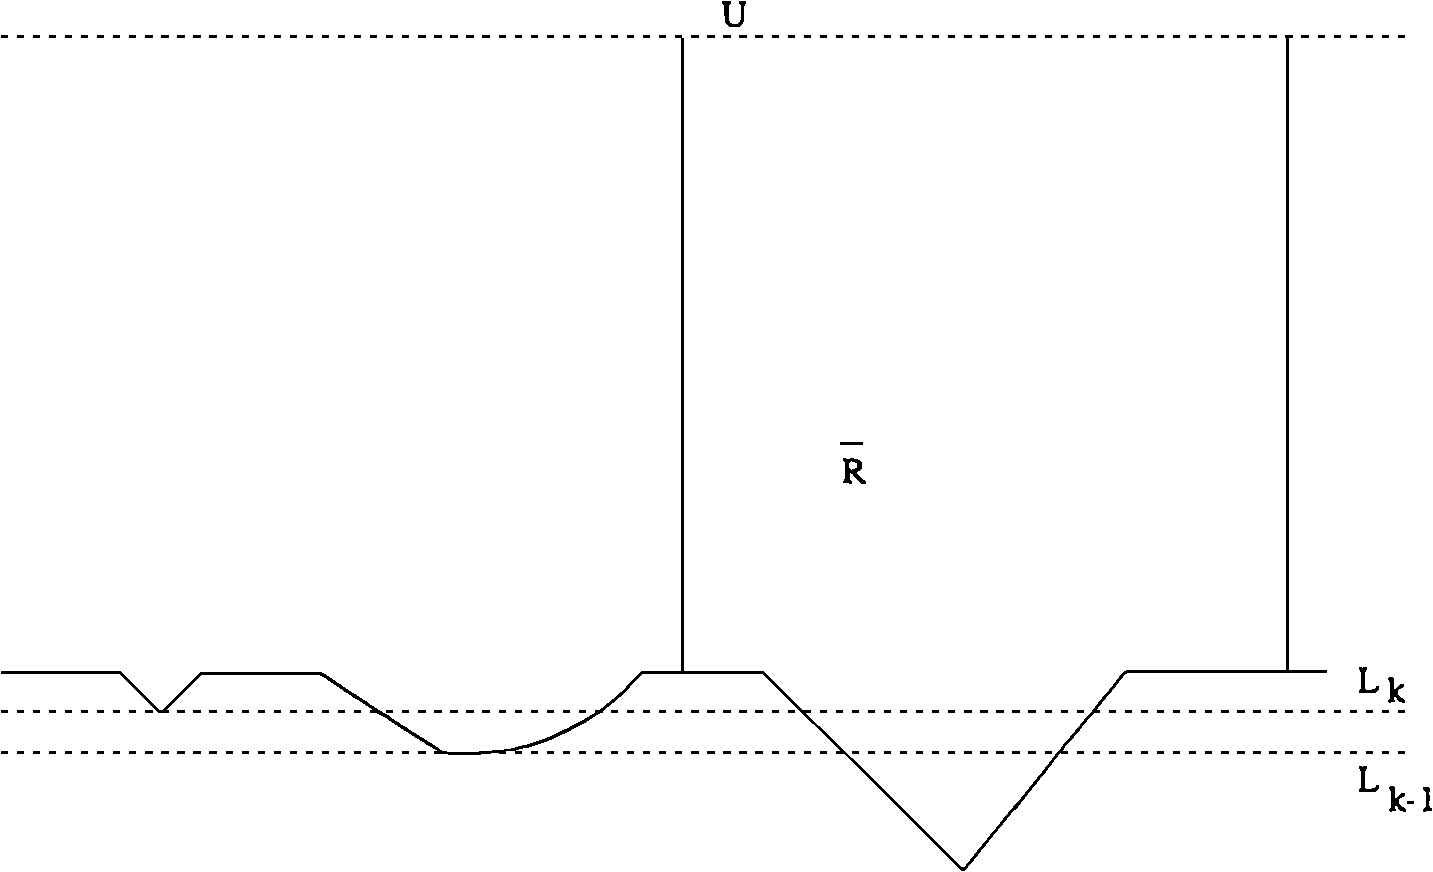
\includegraphics{Images/Img12.png}
    \bigskip
    \caption{Diagram for Theorem \ref{thm:ch5_5.8}.}
    \label{fig:ch5_5.1}
\end{figure}

If $T_U < \tau_{\overline{R}}$ and $K = k$, this means $Z_t$ hits $L_k \cap \overline{R}$ and then hits $U$ before hitting $L_{k-1}$. By the strong Markov property, this is less than or equal to
\begin{align}\label{eq:ch5_5.23}
    \P^x(Z_{S_k} \in L_k \cap \overline{R},\,&T_U \circ \theta_{S_k} < S_{k-1}) \\
    &= \E^x\big[\P^{Z_{S_k}}(T_U < S_{k-1}); Z_{S_k} \in L_k \cap \overline{R}\big]. \notag
\end{align}
If $y \in L_k$, $\P^y(T_U < S_{k-1}) \leq c2^{-k}$. Now
\mpagebreak
\begin{align}\label{eq:ch5_5.24}
    \int \P^x(Z_{S_k} \in L_k \cap \overline{R})\overline{\mu}(dx) &= c \int_1^2 \int_{L_k \cap \overline{R}} \frac{2^{-k}}{2^{-2k} + |x - w|^2}dw\, dx \\
    &\leq c\int_{L_k \cap \overline{R}} dx. \notag
\end{align}
Substituting \eqref{eq:ch5_5.23} and \eqref{eq:ch5_5.24} in \eqref{eq:ch5_5.22} and summing over $k$,
\begin{equation}\label{eq:ch5_5.25}
    \P^x(T_U < \tau_{\overline{R}}) \leq c\sum_{k} 2^{-k}|L_k \cap \overline{R}|.
\end{equation}
By Exercise \ref{ex:ch5_22}, the right-hand side is less than or equal to $c\int_{1/2}^4 F(x)dx$. This gives \eqref{eq:ch5_5.21}.
\end{proof}

\subsecbkm{ch5_sec5.5}{More general domains}

Our main result of the section is the following.

\begin{theorem}\label{thm:ch5_5.11}
Suppose $h$ is a Lipschitz function bounded by $1$ with Lips\-chitz constant at most $1$ and $h(0) = 0$. Suppose $h'(0)$ exists and is equal to $0$. Let $D$ be the region above the graph of $h$. If $J^- = \int_{-\infty}^\infty h^-(x)/x^2 dx < \infty$, then $D$ has an angular derivative at $0$ if and only if $J^+ = \int_{-\infty}^{\infty} h^+(x)/x^2 dx \allowbreak < \infty$.
\end{theorem}

Here $h^+$ and $h^-$ are the positive and negative parts of $h$. Note that the finiteness of $J^+$ and $J^-$ implies $h(0) = 0$ and $h'(0) = 0$.

It can also be shown (\cite{Burdzy1987}) that under the above hypotheses on $h$, if $J^- = \infty$ and $J^+ < \infty$, then the angular derivative does not exist at $0$.\index{Burdzy's theorem}

\begin{proof}
Let $D_1 = D \cap H$, $D_2 = D \cup H$. Suppose first that both integrals $J^-$ and $J^+$ are finite. Let $w_0 \in D$. By Theorems \ref{thm:ch5_5.6} and \ref{thm:ch5_5.8}, $g_{D_1}(\im y,w_0)/y$ and $g_{D_2}(\im y,w_0)/y$ both converge as $y \downarrow 0$ to finite nonzero constants. Since $D_1 \subseteq D \subseteq D_2$, the $\lim \sup$ and $\lim \inf$ of $g_D(\im y,w_0)/y$ are positive and finite. By Proposition \ref{prop:ch5_5.5} in $D_1 \cap B(0,1)$ with $u(z) = g_D(z,w_0)$, we see that $g_D(\im y,w_0)/g_{D_1}(\im y,w_0)$ converges to a positive finite limit as $y \downarrow 0$. Multiplying by $g_{D_1}(\im y,w_0)/y$ implies that $g_D(\im y,w_0)/y$ has a positive finite limit. By Proposition \ref{prop:ch5_5.4}, the angular derivative exists.

Now suppose $J^- < \infty$ but $J^+ = \infty$. Let $U = \{x + \im y : y = 10\}$, let $h(z) = \P^z(T_U < \tau_{D \cup H})$, and let $k(z) = \P^z(T_U < \tau_H) = c\Im z$. Since $H \subseteq H \cup D$, then $h(z) \geq k(z)$. Since $J^- < \infty$, then $h(\im y)/k(\im y) = ch(\im y)/y$ is bounded above and below for $y$ near $0$ by Theorem \ref{thm:ch5_5.8}.

For each $n$,
\mpagebreak
\begin{align*}
    \P_h^{\im y}&(T_{(H-D) \cap B(0,1/n)} < T_U) \\
    &\geq \E^{\im y}[h(Z_{T_U}); T_{(H-D) \cap B(0,1/n)} < T_U < \tau_{D \cup H}]/h(\im y) \\
    &\geq c\E^{\im y}[k(Z_{T_U}); T_{(H-D) \cap B(0,1/n)} < T_U < \tau_H]/k(\im y) \\
    &\geq c\P_k^{\im y}(T_{(H-D) \cap B(0,1/n)} < T_U),
\end{align*}
$c$ independent of $n$. Hence by Exercise \ref{ex:ch5_20}
\begin{equation}\label{eq:ch5_5.26}
    \P_h^0(T_{(H-D) \cap B(0,1/n)} < T_U) \geq c\P_k^0(T_{(H-D) \cap B(0,1/n)} < T_U).
\end{equation}

Since $J^+ = \infty$, it follows from the proof of Theorem \ref{thm:ch5_5.6}
\[
    \P_k^0(T_{(H-D) \cap B(0,1/n)} = 0) > 0
\]
for each $n$. The conclusion of the zero-one law (Corollary \chapref[I]{cor:ch1_3.6}) still holds for $(\P_k^0,Z_t)$ because the same proof works. Hence
\[
    \P_k^0(T_{(H-D) \cap B(0,1/n)} = 0) =1
\]
for each $n$. Using \eqref{eq:ch5_5.26},
\[
    \P_h^0(T_{(H-D) \cap B(0,1/n)} < T_U) > c,
\]
where $c$ is independent of $n$. By the continuity of the paths of $Z_t$ under $\P_h^0$, the Borel-Cantelli lemma, and the fact that $Z_t$ is never equal to $0$ for $t > 0$ under $\P_h^0$, we see that $\P_h^0(T_{H-D} = 0) \geq c$. By the conclusion of the zero-one law (Corollary \chapref[I]{cor:ch1_3.6}) for $(P_h^0,Z_t)$ as above, $\P_h^0(T_{H-D} = 0) = 1$. It follows (Exercise \ref{ex:ch5_20}) that if $\epsilon > 0$, then for $y$ sufficiently small, $\P_h^{\im y}(\tau_D > T_U) \leq \epsilon$, hence
\[
    \P^{\im y}(T_U < \tau_D)\leq c\epsilon y.
\]

Finally, by the boundary Harnack principle in $D$, $g_D(z,w_0)$ and $\P^z(T_U < \tau_D)$ are comparable for $z$ near $0$. Since $\epsilon$ is arbitrary, $g_D(\im y,w_0)/y \allowbreak\to 0$ as $y \downarrow 0$. By Proposition \ref{prop:ch5_5.4}, the angular derivative does not exist at $0$.
\end{proof}

A comparison theorem holds for the angular derivative: if $D_1 \subseteq D \subseteq D_2$ and $D_1$ and $D_2$ both have angular derivatives at $0$, then so does $D$. The existence of the angular derivative is a local property: if $D_1$ has an angular derivative at $0$ and $D_1 \cap B(0,r) = D_2 \cap B(0,r)$ for some $r$, then $D_2$ has an angular derivative at $0$. These two facts, the proofs of which can be found in \cite{Burdzy1987}, together with Theorem \ref{thm:ch5_5.11}, allow one to settle the question of the existence of the angular derivative for many interesting domains; see \cite{Burdzy1987} for details.

Analytic proofs of Burdzy's results can be found \cite{RodinWarschawski1986}, \cite{Carroll1988}, \cite{Gardiner1991}, and \cite{Sastry1993}. In the analysis literature, the angular derivative problem is sometimes converted to a problem concerning the behavior at $\infty$ of a domain contained in a strip by means of the mapping $z \to (-1/\pi)\log z$.

\mpagebreak

The proofs given above for the finiteness and positivity of the normal derivative of the Green function can be easily modified to cover the case when the dimension is greater than $2$; see \cite{Burdzy1987}.

There are still many cases where the angular derivative problem has not been solved. Even the case of domains above Lipschitz functions is still open.

\section{The corona problem}\label{ch5_sec6}

\subsecbkm{ch5_sec6.1}{Maximal ideals}

In this section we give a proof of the famous corona theorem. There are several proofs; the proof we give is due to \cite{Varopoulos1980b}. The first thing we want to do is to reduce the statement of the corona theorem to a concrete problem concerning the existence of a solution to a certain functional equation (Theorem \ref{thm:ch5_6.2}). We then prove the probabilistic analog of this equation (Theorem \ref{thm:ch5_6.7}), and finally deduce the analytic result from the probabilistic one.

Let $H^\infty$\index{H3@$H^\infty$} be the set of functions that are analytic on $\D$ and bounded on $\overline{\D}$. $H^\infty$ is an algebra under the operation of pointwise multiplication. $M$ is an ideal in this algebra if $M$ is a subring of $H^\infty$ and $f \in M$ and $g \in H^\infty$ implies $fg \in M$. Any ideal containing the constant function $1$ is, of course, equal to $H^\infty$ itself. If $z \in \D$, $M_z = \{f \in H^\infty : f(z) = 0\}$ is an example of an ideal, and in fact, $M_z$ is a maximal ideal\index{Maximal ideal}. That is, it is a proper subset of $H^\infty$ and is not properly contained in any other proper ideal (see Exercise \ref{ex:ch5_24}). If $\MC$ denotes the set of maximal ideals, $z \to M_z$ is an embedding of $\D$ into $\MC$. In a moment we will discuss a topology on $\MC$. The corona theorem is the assertion that in this topology, $\overline{\D} = \MC$. $\MC - \overline{\D}$ is what is left over if the face of the sun ($\MC$) is obscured by the shadow of the moon ($\overline{\D}$) during a full eclipse, the corona\index{Corona} of the sun. The corona theorem says that the corona is empty.

To put a topology on $\MC$, we need to very briefly discuss the Gel'fand mapping.

\begin{proposition}\label{prop:ch5_6.1}
If $M \in \MC$, then $H^\infty/M$ is isomorphic to $\C$. Let $f(M) = f + M$ denote the mapping from $H^\infty$ to $\C$. Then the mapping is linear, $fg(M) = f(M)g(M)$, $|f(M)| \leq \|f\|_\infty$, $1(M) = 1$, and $f(M) = 0$ if and only if $f \in M$.
\end{proposition}

Here $|f(M)| = \|f + M\| = \inf_{g\in M} \|f + g\|_\infty$.

\begin{proof}
Let us first show that $M$ is closed. Since the closure of an ideal is also an ideal, and $M$ is maximal, either $M = \overline{M}$ or $\overline{M} = H^\infty$. Let us show that the latter case cannot happen. If $1 \in \overline{M}$, there must exist $g \in M$ with $\|1 - g\| < 1$. Then the series $\sum_{n=0}^\infty(1-g)^n$ converges absolutely, and is equal to $g^{-1}$, since
\[
    g\sum_{n=0}^\infty(1-g)^n = [1-(1-g)]\sum_{n=0}^\infty(1-g)^n = 1.
\]
So $g^{-1} \in H^\infty$ and therefore $1 = gg^{-1} \in M$, contradicting the fact that $M$ is proper. Therefore $M$ is closed.

Let $B = H^\infty/M$, the quotient algebra. Since $M$ is maximal, $B$ is a field (Exercise \ref{ex:ch5_23}). We want to show it is isomorphic to $\C$. Suppose it is not. Then there exists $f \in B$ such that $f \neq \lambda + M$ for any $\lambda \in \C$. $(f - \lambda)$ is an element of $B$ that is not $0$, hence it has an inverse. Thus $(f - \lambda)^{-1} \in B$ for all $\lambda \in \C$. Clearly $f^{-1} \neq 0$, and by the Hahn-Banach theorem, there exists a bounded linear functional on $B$ such that $\|L\| = 1$ and $L(f^{-1}) \neq 0$.

Provided $|\lambda - \lambda_0| < 1/\|(f - \lambda_0)^{-1}\|$,
\[
    (f - \lambda)^{-1} = \sum_{n=0}^\infty(\lambda - \lambda_0)^n((f - \lambda_0)^{-1})^{n+1}.
\]
Then defining $F(\lambda) = L((f - \lambda)^{-1})$,
\[
    F(\lambda) = \sum_{n=0}^\infty L(((f - \lambda_0)^{-1})^{n+1})(\lambda - \lambda_0)^n.
\]
Since $\|L\| = 1$, the series converges uniformly, and still provided $|\lambda - \lambda_0| < 1/\|(f - \lambda_0)^{-1}\|$, $F$ is analytic. So $F$ is analytic in some neighborhood of any point $\lambda_0$, and therefore $F$ is entire.

Now if $|\lambda|$ is sufficiently large,
\[
    (f - \lambda)^{-1} = \frac{1}{\lambda}\sum \frac{f^n}{\lambda^n},
\]
and
\[
    |F(\lambda)| = |L((f - \lambda)^{-1})| \leq \frac{1}{|\lambda|}\sum \frac{\|f\|^n}{|\lambda|^n} \leq \frac{c}{|\lambda|}.
\]
By the maximum modulus theorem, for each $N$, $\sup_{|\lambda| \leq N} |F(\lambda)| \leq c/N$, from which we conclude $F \equiv 0$. We know, however, that $L(f^{-1}) \neq 0$, a contradiction. Therefore $B$ is isomorphic to $\C$.

The only remaining part of the proposition that takes some work is the assertion that $|f(M)| \leq \|f\|_\infty$. Suppose $f \in H^\infty$ with $\|f\|_\infty < 1$ but $|f(M)| = 1$. By looking at $e^{i\theta}f$ for suitable $\theta$, we may assume $f(M) = 1$. Then $(1-f)^{-1}$ exists and equals $\sum_{n=0}^\infty f^n$. Then
\[
    1 = 1(M) = (1-f)^{-1}(M)(1(M) - f(M)) = 0,
\]
a contradiction.
\end{proof}

For $f \in H^\infty$, define the Gel'fand transform $f \to \widehat{f}$ by letting $\widehat{f}$ map $\MC$ into $\C$ with $\widehat{f}(M) = f(M)$. Define a topology on $\MC$ by defining a basic neighborhood of $M' \in \MC$ to be a set of the form
\[
    V = \{M \in \MC : |\widehat{f}_j(M) - \widehat{f}_j(M')| < \epsilon, 1 \leq j \leq n\}
\]
for some $\epsilon > 0$ and $f_1,\ldots,f_n \in H^\infty$.

The main project in this section is to prove the following.

\begin{theorem}\label{thm:ch5_6.2}
Suppose $\delta > 0$, $n > 1$, and $f_1,\ldots,f_n \in H^\infty$ with
\begin{equation}\label{eq:ch5_6.1}
    \max_{1\leq j\leq n} |f_j(z)| \geq \delta, \qquad z \in \D.
\end{equation}
Then there exist $g_1,\ldots,g_n \in H^\infty$ such that
\begin{equation}\label{eq:ch5_6.2}
    f_1(z)g_1(z) + \cdots + f_n(z)g_n(z) = 1, \qquad z \in \D.
\end{equation}
\end{theorem}

The $f_j$ are called corona data and the $g_j$ corona solutions\index{Corona solutions}. As a corollary, we have the corona theorem\index{Corona theorem}.

\begin{corollary}\label{cor:ch5_6.3}
$\D$ is dense in $\MC$.
\end{corollary}

\begin{proof}[Proof of the corollary]
Suppose $\{M_z; z \in \D\}$ is not dense in $\MC$. Then there exists $N \in \MC$ and a neighborhood $V$ of $N$ of the form $V = \{M \in \MC : |\widehat{h}_j(M) - \widehat{h}_j(N)| < \delta, j=1,\ldots,n\}$ that contains no $M_z$, where $h_1,\ldots,h_n \in H^\infty$. Let $f_j = h_j - \widehat{h}_j(N)\cdot 1$. Then $f_j \in H^\infty$ and $V = \{M \in \MC : |f_j(M)| < \delta, j=1,\ldots,n\}$. Moreover, $\widehat{f}_j(N) = \widehat{h}_j(N) - \widehat{h}_j(N) = 0$, so each $f_j$ is in $N$. If $z \in \D$, then since $M_z \notin V$, $|f_j(z)| \geq \delta$ for at least one $j$.

Since $N$ is an ideal, $1 = f_1g_1 + \cdots + f_ng_n \in N$, where the $g_1,\ldots,g_n$ are given by Theorem \ref{thm:ch5_6.2}. This contradicts $N$ being proper.
\end{proof}

\subsecbkm{ch5_sec6.2}{Holomorphic martingales}

Let us return to the situation where $Z_t$ is two-dimensional Brownian motion. In this section we need to distinguish between complex-valued Brownian motion and $\R^2$-valued Brownian motion, so we write $Z_t = \Re Z_t + \im\Im Z_t$ and we let $\widehat{Z}_t$ denote the vector $(\Re Z_t, \Im Z_t)$.

\index{Holomorphic martingales|(}

\begin{definition}\label{def:ch5_6.4}
A complex-valued process $M_t$ is a holomorphic martingale if $\sup_t |M_t| \in L^p$ and $M_t = M_0 + \int_0^t H_s dZ_s$ for some predictable complex-valued process $H_s$.
\end{definition}

As one would expect, $\int_0^t H_s dZ_s$ is defined to be
\mpagebreak
\begin{align}\label{eq:ch5_6.3}
    \int_0^t (\!&\Re H_s + \im\Im H_s)d(\Re Z_s + \im\Im Z_s) \\
    &= \int_0^t (\Re H_s d\Re Z_s - \Im H_s d\Im Z_s) \notag \\
    &\qquad+ \im\int_0^t (\Re H_s d\Im Z_s + \Im H_s d\Re Z_s). \notag
\end{align}

The prototypes for holomorphic martingales are $M_t = f(Z_t)$ where $f$ is analytic. If we write $f = u + \im v$, then $u$ and $v$ are harmonic, and by It\^o's formula,
\[
    u(Z_t) = u(Z_0) + \int_0^t \big(\partial_x u(Z_s)d\Re Z_s + \partial_y u(Z_s)d\Im Z_s\big),
\]
and similarly for $v(Z_t)$. So by the Cauchy-Riemann equations
\begin{align}\label{eq:ch5_6.4}
    f(Z_t) &= (u + \im v)(Z_t) \\
    &= f(Z_0) + \int_0^t (\partial_x u + \im\partial_x v)(Z_s)d\Re Z_s \notag \\
    &\qquad+ \int_0^t (\partial_y u + \im\partial_y v)(Z_s)d\Im Z_s \notag \\
    &= f(Z_0) + \int_0^t H_s dZ_s, \notag
\end{align}
where $H_s = (\partial_x u)(Z_s) + \im(\partial_x v)(Z_s) = f'(Z_s)$.

Just as with analytic functions, the real and imaginary parts of holomorphic martingales are closely tied together.

\begin{lemma}\label{lem:ch5_6.5}
Suppose
\begin{equation}\label{eq:ch5_6.5}
    \Re M_t = \Re M_0 + \int_0^t K_s \cdot d\widehat{Z}_s
\end{equation}
for some $K_s$ predictable. Then $M_t$ is a holomorphic martingale if and only if
\begin{equation}\label{eq:ch5_6.6}
    \Im M_t = \Im M_0 + \int_0^t AK_s \cdot d\widehat{Z}_s,
\end{equation}
where
\begin{equation}\label{eq:ch5_6.7}
A = \begin{pmatrix} 0 & -1 \\ 1 & 0 \end{pmatrix}.
\end{equation}
\end{lemma}

\begin{proof}
We may suppose without loss of generality that $M_0 = 0$. Suppose $M_t$ is holomorphic martingale, so that $M_t = \int_0^t H_s dZ_s$. Then
\mpagebreak
\[
    \Re M_t = \int_0^t [\Re H_s d\Re Z_s - \Im H_s d\Im Z_s]
\]
and
\[
    \Im M_t = \int_0^t [\Im H_s d\Re Z_s + \Re H_s d\Im Z_s].
\]
Hence $K_s = \begin{pmatrix} \Re H_s \\ -\Im H_s \end{pmatrix}$ and $AK_s = \begin{pmatrix} \Im H_s \\ \Re H_s \end{pmatrix}$, and so indeed $\Im M_t = \int_0^t AK_s \cdot d\widehat{Z}_s$.

Conversely, suppose \eqref{eq:ch5_6.5} and \eqref{eq:ch5_6.6} hold. If $K_s = \begin{pmatrix} B_s \\ C_s \end{pmatrix}$, we let $H_s = B_s - \im C_s$, and see that $M_t = \int_0^t H_s dZ_s$.
\end{proof}

We define the space $\HC^p$\index{H4@$\HC^p$}, $1 \leq p \leq \infty$, to be the set of holomorphic martingales $M_t$ such that $\sup_{t<\infty} |M_t| \in L^p$. We are especially interested in the spaces $\HC^\infty$. We saw that if $f \in H^\infty$, then $f(Z_{t\wedge\tau_D}) \in \HC^\infty$. One of the key ideas is how to construct an analytic function from an $\HC^\infty$ martingale.

\index{Holomorphic martingales|)}

\begin{proposition}\label{prop:ch5_6.6}
Suppose $M \in \HC^\infty$. Let $f$ be a function whose real and imaginary parts are harmonic in $\D$ and $f$ has boundary values $f(e^{\im\theta}) = \E_\theta^0M_\tau$. Then $f \in H^\infty$.
\end{proposition}

This could be expressed as $f(e^{\im\theta}) = \E^0[M_\tau\mid Z_\tau = e^{\im\theta}]$. Saying that $f$ has boundary values $f(e^{\im\theta})$ means that the nontangential limits of the real and imaginary parts of $f$ are equal to the real and imaginary parts of $f(e^{\im\theta})$ for almost every $\theta$.

\begin{proof}
It is clear that $f$ is bounded. What we need to show is that $f$ is analytic in $\D$. Write $u = \Re f$ and $v = \Im f$. By Lemma \ref{lem:ch5_6.5}, $\Re M_\tau = \int_0^\tau K_s d\widehat{Z}_s$ and $\Im M_\tau = \int_0^\tau AK_s d\widehat{Z}_s$ where $A$ is the matrix given by \eqref{eq:ch5_6.7} and $K_s$ is some predictable process.

Suppose $h$ is a $L^2$ function on $\partial\D$ and let $h$ also denote its harmonic extension. Let $\widetilde{h}$ denote the conjugate harmonic function to $h$. By Exercise \ref{ex:ch5_25}, the nontangential limit of $\widetilde{h}$ exists at almost every point of the boundary; if we denote the boundary values by $\widetilde{h}$ also, then $\widetilde{h} \in L^2(\partial\D)$. Then
\begin{align*}
    \frac{1}{2\pi} \int_0^{2\pi} v(e^{\im\theta})h(e^{\im\theta})d\theta &= \E^0[v(Z_\tau)h(Z_\tau)] \\
    &= \E^0[(\Im M_\tau)h(Z_\tau)]
\end{align*}
by Proposition \chapref[III]{prop:ch3_2.7}. Since $\Im M_t$ and $h(Z_t)$ are both martingales, the integration by parts formula shows this is equal to
\begin{align*}
    \E^0\lrang{\Im M,h(Z)}_t &= \E^0 \int_0^\tau AK_s \cdot \nabla h(Z_s)ds \\
    &= \E^0 \int_0^\tau (A^t\nabla h)(Z_s) \cdot K_s ds.
\end{align*}

\mnewpage

Now $A^t\nabla h = -\nabla\widetilde{h}$. So reversing the above calculation, this is equal to
\[
    -\E^0 \int_0^\tau (\nabla\widetilde{h})(Z_s) \cdot K_s ds = -\E^0[(\Re M_\tau)\widetilde{h}(Z_\tau)] = -\E^0[u(Z_\tau)\widetilde{h}(Z_\tau)].
\]

Let $u$ be the harmonic extension of $u$ and let $\widetilde{u}$ be the conjugate harmonic function to $u$. Then similarly, since $u(Z_t)$ and $v(Z_t)$ are martingales,
\begin{align*}
    \E^0[\widetilde{u}(Z_\tau)h(Z_\tau)] &= \E^0\lrang{\widetilde{u}(Z)h(Z)}_\tau \\
    &= \E^0 \int_0^\tau \nabla\widetilde{u}(Z_s) \cdot \nabla h(Z_s)ds \\
    &= \E^0 \int_0^\tau (A\nabla u)(Z_s) \cdot \nabla h(Z_s)ds \\
    &= \E^0 \int_0^\tau \nabla u(Z_s) \cdot (A^t\nabla h)(Z_s)ds \\
    &= -\E^0 \int_0^\tau \nabla u(Z_s) \cdot \nabla \widehat{h}(Z_s)ds.
\end{align*}
Reversing the calculation, we see that this is $-\E^0[u(Z_\tau)\widetilde{h}(Z_\tau)]$.

We conclude $\int_0^{2\pi} v(e^{\im\theta})h(e^{\im\theta})d\theta = \int_0^{2\pi} \widetilde{u}(e^{\im\theta})h(e^{\im\theta})d\theta$ whenever $h$ is in $L^2(\partial\D)$. It follows that $v = \widetilde{u}$ a.e., which shows that the harmonic extension of $v$ is the conjugate harmonic function to $u$, or $u + \im v$ is analytic.
\end{proof}

We can now state the corona theorem\index{Corona theorem} for martingales.

\begin{theorem}\label{thm:ch5_6.7}
Suppose $F_1,\ldots,F_n \in \HC^\infty$ and there exists $\delta > 0$ such that
\[
    \max_{1\leq j\leq n} |F_j(t)| > \delta, \qquad \textnormal{a.s.},
\]
for each $t$. Then there exist $G_1,\ldots,G_n \in \HC^\infty$ such that
\[
    F_1G_1 + \cdots + F_nG_n = 1, \qquad \textnormal{a.s.},
\]
for all $t$.
\end{theorem}

A first guess would be to let $G_j(t) = \overline{F}_j(t)/\sum|F_j(t)|^2$, where $\overline{F}_j$ is, of course, the complex conjugate. There is no reason to expect $G_j$ to be holomorphic, and what we do instead is look at $\overline{F}_j(t)/\sum|F_j(t)|^2 + \sum_{k=1}^n W_{jk}(t)F_k(t)$ for suitable $W$.

Let us set $F(t) = (F_1(t),\ldots,F_n(t))$ and let $\overline{F}(t) = (\overline{F}_1(t),\ldots,\overline{F}_n(t))$ be the complex conjugates. $F_j(t)$ is holomorphic, and we denote by $F'_j(t)$ the predictable process such that $F_j(t) = F_j(0) + \int_0^t F'_j(t) dZ_t$. $F'(t)$ and $\overline{F}'(t)$ are the corresponding vectors. $\|F(t)\|$ will denote $(\sum_{j=1}^n |F_j(t)|^2)^{1/2}$. Let
\begin{equation}\label{eq:ch5_6.8}
    L_j(t) = \overline{F}_j(t)/\|F(t)\|^2.
\end{equation}

Note since $\Re Z_s$ and $\Im Z_s$ are independent, $d\lrang{\Re Z,\Im Z}_t = 0$, or
\begin{equation}\label{eq:ch5_6.9}
    d\lrang{Z,Z}_t = 0, \qquad d\lrang{Z,\overline{Z}}_t = 2\,dt.
\end{equation}

We need some lemmas.

\begin{lemma}\label{lem:ch5_6.8}
\[
    L_j(t) = L_j(0) + \int_0^t A_j(t)dZ_t + \int_0^t B_j(t)d\overline{Z}_t + \int_0^t C_j(t)dt,
\]
where
\[
    A_j(t) = -\overline{F}_j(t)\frac{\overline{F}(t) \cdot F'(t)}{\|F(t)\|^4},
\]
\[
    B_j(t) = \frac{F'_j(t)}{\|F(t)\|^2} - \overline{F}_j(t)\frac{F(t) \cdot \overline{F}'(t)}{\|F(t)\|^4},
\]
and
\[
    C_j(t) = \overline{F}_j(t)\frac{4|F(t) \cdot F'(t)|^2 - 2\|F(t)\|^2\|F''(t)\|^2}{\|F(t)\|^6} - 2\overline{F}'_j(t)\frac{\overline{F}(t) \cdot F'(t)}{\|F(t)\|^4}.
\]
\end{lemma}

\begin{proof}
It is easier to compute $\overline{L}_j(t)$ and then take complex conjugates. Let
\[
    H(t) = \|F(t)\|^2 = \sum|F_j(t)|^2 = \sum F_j(t)\overline{F}_j(t).
\]
By It\^o's formula and \eqref{eq:ch5_6.9},
\begin{align}\label{eq:ch5_6.10}
    dH(t) &= \sum F_j(t)d\overline{F}_j(t) \\
    &\qquad+ \sum \overline{F}_j(t)dF_j(t) + \sum \lrang{F_j,\overline{F}_j}_t \notag \\
    &= \sum F_j(t)\overline{F}'_j(t)d\overline{Z}_t + \sum \overline{F}_j(t)F'_j(t)dZ_t \notag \\
    &\qquad+ 2\sum F'_j(t)\overline{F}'_j(t) dt. \notag
\end{align}
Then
\begin{equation}\label{eq:ch5_6.11}
    d\lrang{H}_t = 2(F(t) \cdot F'(t))(\overline{F}(t) \cdot F'(t))dt.
\end{equation}
If $K = H^{-1}$,
\begin{equation}\label{eq:ch5_6.12}
    dK(t) = -H(t)^{-2}dH(t) + 2H(t)^{-3}d\lrang{H}_t.
\end{equation}
Also,
\begin{equation}\label{eq:ch5_6.13}
    d\overline{L}_j(t) = F_j(t)dK(t) + K(t)dF_j(t) + d\lrang{F_j,K}_t.
\end{equation}
Combining \eqref{eq:ch5_6.10}, \eqref{eq:ch5_6.11}, \eqref{eq:ch5_6.12}, and \eqref{eq:ch5_6.13} and taking complex conjugates proves the lemma.
\end{proof}

A random variable $U$ is said to be in $\BMO$\index{BMO2@$\BMO$} if the martingale $\E[U\mid \FC_t]$ is in $\BMO$.

\begin{lemma}\label{lem:ch5_6.9}
Suppose
\[
    X_t = X_0 + \int_0^t A_s d\Re Z_s + \int_0^t B_s d\Im Z_s
\]
is in $\BMO$. Suppose $H_s$ is predictable and $\sup_s |H_s| \leq c < \infty$, a.s.
\begin{enumerate}[label=(\alph*)]
    \item The martingales
    \begin{align*}
        \int_0^\tau H_sA_sd\Re Z_s, \quad &\int_0^\tau H_sB_sd\Re Z_s, \quad \int_0^\tau H_sA_sd\Im Z_s, \quad \text{and} \\
        &\quad \int_0^\tau H_sB_sd\Im Z_s
        % Note: \quad is used here
    \end{align*}
    are all in $\BMO$.
    \item The random variables
    \[
        \int_0^\tau H_sA_s^2ds, \quad \int_0^\tau H_sA_sB_sds, \quad \text{and} \quad \int_0^\tau H_sB_s^2ds
        % Note: \quad is used here
    \]
    are all in $\BMO$.
\end{enumerate}
\end{lemma}

\begin{proof}
All the stochastic integral terms in (a) are similar. Let us look at
\[
    Y_t = \int_0^t H_sA_sd\Re Z_s.
\]
Then
\begin{align*}
    \E[|Y_\tau - Y_t|^2\mid \FC_t] &= \E\Big[\int_t^\tau H_s^2A_s^2ds\mid\FC_t\Big] \leq c\E\Big[\int_t^\tau [A_s^2 + B_s^2]ds\mid\FC_t\Big] \\
    &= c\E\big[|X_T - X_t|^2\mid \FC_t\big] \leq c\|X\|^2_{\BMO}.
\end{align*}

The three terms in (b) are similar. Let us let $U_\tau = \int_0^\tau H_sA_sB_sds$ and $U_t = \E[U_\tau\mid \FC_t]$. Then if $t < \tau$,
\begin{align*}
    \E[|U_\tau - U_t|\mid \FC_t] &= \E\Big[\Big|\int_t^\tau H_sA_sB_sds - \E\Big[\int_t^\tau H_sA_sB_sds\mid \FC_t\Big]\Big|\mid \FC_t\Big] \\
    &\leq 2\E\Big[\int_t^\tau |H_sA_sB_s|ds\mid \FC_t\Big] \\
    &\leq c\E\Big[\int_t^\tau [A_s^2 + B_s^2]ds\mid \FC_t\Big].
\end{align*}
As above, this is bounded by $c\|X\|^2_{\BMO}$. By Theorem \chapref[I]{thm:ch1_6.11} and Exercise \ref{ex:ch5_26}, $U_\tau \in \BMO$.
\end{proof}

\begin{lemma}\label{lem:ch5_6.10}
Suppose $N \in \BMO$ and $\E[NM_\infty] = 0$ for all $M \in \HC^2$. Then $N \in \HC^2$.
\end{lemma}

\begin{proof}
Since $N \in \BMO$, then $N \in \MC^2$, and we need to show that $N$ is holomorphic. Let $N_t = \E[N\mid \FC_t]$. By the martingale representation theorem (Corollary \chapref[I]{cor:ch1_5.14}), $N_t = N_0 + \int_0^t a_sd\Re Z_s + \int b_sd\Im Z_s$ for some $a_s$, $b_s$ predictable and complex-valued. If we set $A_s = (a_s - \im b_s)/2$ and $B_s = (a_s + \im b_s)/2$, then
\[
    N_t = N_0 + \int_0^t A_sdZ_s + \int_0^t B_sd\overline{Z}_s.
\]

Let $M_t = \int_0^t S_sdZ_s$ where $S_s$ is predictable, bounded, and $0$ after some fixed time $t_0$. Then $M_t \in \HC^2$ and
\[
    0 = \E[NM_\infty] = \E\lrang{N,M}_\infty = 2\int_0^\infty B_sS_sds,
\]
using \eqref{eq:ch5_6.9}. Since this holds for all such $S_s$, then $B_s = 0$, a.s.\ for almost every $s$, or $N_t = \int_0^t A_sdZ_s$ is holomorphic.
\end{proof}

\begin{proof}[Proof of Theorem 6.7]
Let
\begin{equation}\label{eq:ch5_6.14}
    H_{jk}(t) = \frac{\overline{F}_j(t)F'_k(t) - \overline{F}_k(t)F'_j(t)}{\|F(t)\|^4}
\end{equation}
and
\begin{equation}\label{eq:ch5_6.15}
    K_{jk}(t) = 4\frac{F(t) \cdot F'(t)}{\|F(t)\|^6}[\overline{F}_k(t)F'_j(t) - \overline{F}_j(t)F'_k(t)].
\end{equation}
Note both $H_{jk}$ and $K_{jk}$ are antisymmetric.

Let
\[
    U_{jk}(t) = \int_0^t H_{jk}(s)d\overline{Z}_s + \int_0^t K_{jk}(s)ds.
\]
By Lemma \ref{lem:ch5_6.9}, $\E[|U_{jk}(\infty)\mid \FC_t] \in \BMO$. By Fefferman's inequality (Proposition \chapref[IV]{prop:ch4_7.4}),
\[
    L(M) = \E[U_{jk}(\infty)M_\infty]
\]
is a bounded linear functional on $\MC^1$. Since $\MC^1 \subseteq L^1(dP)$, we can extend $L$ to a bounded linear functional on $L^1(dP)$. There thus exists a complex-valued random variable $V_{jk} \in L^\infty(dP)$ such that
\[
    L(M) = \E[V_{jk}M_\infty]
\]
for all $M \in \HC^1$, and hence
\[
    \E[U_{jk}(\infty)M_\infty] = \E[V_{jk}M_\infty]
\]
for all $M \in \HC^1$.

\mpagebreak

Recall $U_{jk}$ is antisymmetric. We may assume without loss of generality that $V_{jk}$ is also antisymmetric, for if we replace $V_{jk}$ by $V'_{jk} = (V_{jk} - V_{kj})/2$,
\begin{align*}
    \E[V'_{jk}M_\infty] &= (\E[V_{jk}M_\infty] - \E[V_{kj}M_\infty])/2 \\
    &= (\E[U_{jk}(\infty)M_\infty] - \E[U_{kj}(\infty)M_\infty])/2
    &= \E[U_{jk}(\infty)M_\infty].
\end{align*}

By Lemma \ref{lem:ch5_6.10} and the fact that $\HC^2 \subseteq \HC^1$, we see that $\E[U_{jk}(\infty) - V_{jk}\mid \FC_t]$ is holomorphic.

Next we define
\begin{equation}\label{eq:ch5_6.16}
    W_{jk}(t) = -\E[U_{jk}(\infty) - V_{jk}\mid \FC_t] + \int_0^t H_{jk}(s)d\overline{Z}_s + \int_0^t K_{jk}(s)ds.
\end{equation}
Then $W_{jk}(\infty) = V_{jk} \in L^\infty$.

Finally, let
\[
    G_j(t) = L_j(t) + \sum_{k=1}^n W_{jk}(t)F_k(t).
\]
Clearly $G_j \in L^\infty$. Since $W_{jk}$ is antisymmetric, $\sum_{j,k} F_j(t)W_{jk}(t)F_k(t) = 0$, and so $\sum_{j=1}^n F_j(t)G_j(t) = 1$. All that remains is to show that the $G_j(t)$ are holomorphic. Making the substitutions, we have
\begin{equation}\label{eq:ch5_6.17}
    dG_j(t) = dL_j(t) + \sum_{k=1}^n[W_{jk}(t)dF_k(t) + F_k(t)dW_{jk}(t) + d\lrang{F_k,W_{jk}}_t].
\end{equation}
In view of \eqref{eq:ch5_6.9} and the fact that $F_k(t)$ and $\E[U_{jk}(\infty) - V_{jk}|\FC_t]$ are holomorphic,
\[
    d\lrang{F_k,W_{jk}}_t = 2F'_k(t)H_{jk}(t) dt.
\]
Substituting this, \eqref{eq:ch5_6.14}, \eqref{eq:ch5_6.15}, and \eqref{eq:ch5_6.17} in \eqref{eq:ch5_6.16} shows $G_j(t)$ is holomorphic.
\end{proof}

\tweakpage{1}

We can now prove Theorem \ref{thm:ch5_6.2}.

\begin{proof}[Proof of Theorem 6.2]
Let $f_j$ be in $H^\infty$ with $\max_{1\leq j\leq n}|f_j(z)| \geq \delta > 0$. Let $F_j(t) = f_j(Z_{t\wedge\tau})$. By Theorem \ref{thm:ch5_6.7}, there exists $G_j$ holomorphic in $\HC^\infty$ such that $\sum_{j=1}^n F_j(t)G_j(t) = 1$. Let $g_j(e^{\im\theta}) = \E_\theta^0G_j(\tau)$. By Proposition \ref{prop:ch5_6.6}, each function $g_j$ equals the boundary values of an analytic function in $H^\infty$; let us denote that function by $g_j$ also. Since $\sum F_j(\tau)G_j(\tau) = 1$, then
\[
    1=\sum \E_\theta^0[F_j(\tau)G_j(\tau)] = \sum \E_\theta^0[f_j(e^{\im\theta})G_j(\tau)] = \sum f_j(e^{\im\theta})g_j(e^{\im\theta})
\]
for almost all $\theta$. Hence $\sum f_j(z)g_j(z) = 1$ for all $z$ in the interior of $\D$.
\end{proof}

The corona theorem has also been proved for many other domains in $\C$. See \cite{Behrens1970,Behrens1971}, \cite{JonesMarshall1985}, and \cite{GarnettJones1985}. It is still an open problem whether the corona is empty for every planar domain. (Where the proof breaks down is in Proposition \ref{prop:ch5_6.6}; in multiply connected domains there is not a single-valued conjugate harmonic function.) There does exist a Riemann surface in which the analog of Theorem \ref{thm:ch5_6.2} fails; \cite[see][Chap.~4]{Gamelin1978}.

The corona theorem was first proved by Carleson as a consequence of his solution of an interpolation problem\index{Interpolation problem}; see \cite{Carleson1962}.

\section{Exercises and further results}\label{ch5_sec7}

\begin{exercise}\label{ex:ch5_1}
Suppose $f$ is entire and nonconstant. Show $\lrang{f(Z)}_t \to \infty$ a.s.\ as $t \to \infty$.

\hint Use the recurrence of two-dimensional Brownian motion.
\end{exercise}

\begin{exercise}\label{ex:ch5_2}
State and prove a version of the Phragm\'en-Lindel\"of theorem\index{Phragm\'en-Lindel\"of theorem} for $W_\alpha$, the wedge of aperture $\alpha$.
\end{exercise}

\begin{exercise}\label{ex:ch5_3}
If $S = \{0 < \Im z < \pi/2\}$ and $z \in S$, find $\P^z(Z_{\tau_S} \in dt)$ for $t \in \{\Im z = 0\}$.
\end{exercise}

\begin{exercise}\label{ex:ch5_4}
Show that the $f$ defined in the proof of Theorem \ref{thm:ch5_1.14} is single-valued.

\hint For $\delta < \dist(z_0,\partial D)/2$, let $\gamma_\delta$ consist of the curve that starts at $z_0 + \im\delta$ and goes once around $B(z_0,\delta)$ clockwise. Let $\Delta_\delta$ be the difference between the starting value and the ending value of $f(z)$ as $z$ follows $\gamma_\delta$ once around. Argue that it suffices to show that $\Delta_\delta = 0$. By connecting $\gamma_\delta$ to $\gamma_\epsilon$ by a straight line segment that is traversed once in each direction, show that $\Delta_\delta = \Delta_\epsilon$ for all $\epsilon < \delta$. Finally, use estimates of $g$ in small neighborhoods of $z_0$ to show $\lim_{\epsilon \to 0} \Delta_\epsilon = 0$.
\end{exercise}

\begin{exercise}\label{ex:ch5_5}
Suppose $\delta > 0$. Suppose $X_n$ is an integer-valued process such that $X_{n+1} - X_n = 1$ or $-1$ with probability 1 and $\P(X_{n+1} - X_n = 1\mid \FC_n) \geq 1/2 + \delta$, a.s., if $X_n > 0$. Show that $X_n \to \infty$ a.s.

\hint Let $P_n = \P(X_{n+1} - X_n = 1\mid \FC_n)$. Let $U_n$ be a sequence of independent identically distributed random variables that are independent of the $X$s and have a uniform distribution on $[0,1]$, that is $\P(U_n < a) = a$ if $a \in [0,1]$. Define $Y_{n+1} = Y_n + 1$ if $X_{n+1} - X_n = +1$ and $U_n < (1/2+\delta)/P_n$. Otherwise let $Y_{n+1} = Y_n - 1$. Show $Y_n$ is the sum of independent identically distributed random variables that take the value $+1$ with probability $1/2+\delta$ and the value $-1$ with probability $1/2-\delta$. Conclude from Exercise \chapref[I.8]{ex:ch1_18} that $Y_n \to \infty$ a.s. Show that $X_n \geq Y_n$, a.s.
\end{exercise}

\begin{exercise}\label{ex:ch5_6}
Suppose that $D$ is a Jordan domain\index{Jordan domain} (so that by \cite{Pommerenke1975} $D$ is the image of $\D$ under a one to one function $f$ that is analytic in $\D$ and continuous on $\partial\D$). Use conformal mapping to show that the Martin boundary\index{Martin boundary} of $D$ may be identified with the Euclidean boundary of $D$. Show that the boundary Harnack principle\index{Boundary Harnack principle} holds in $D$.
\end{exercise}

\mnewpage

\begin{exercise}\label{ex:ch5_7}
Suppose $u$ is a positive harmonic function in $\D$ that converges radially at $e^{\im\theta}$. Show $u$ converges nontangentially at $e^{\im\theta}$.
\end{exercise}

\begin{exercise}\label{ex:ch5_8}
Show that if $M_t$ is a continuous martingale, the two sets $(\lim_{t\to\infty} M_t~\text{exists})$ and $(\lrang{M}_\infty < \infty)$ differ by a set of probability $0$.
\end{exercise}

\begin{exercise}\label{ex:ch5_9}
Show that $f(z) = \sum_{k\geq 0} z^{2^k}$ is a Bloch function.
\end{exercise}

\begin{exercise}\label{ex:ch5_10}
Complete the proof of \eqref{eq:ch5_4.10} in Hall's lemma (that is, consider the cases $\rho \leq 1/2$ and $b \leq 1/2$).
\end{exercise}

\begin{exercise}\label{ex:ch5_11}
Prove a version of Theorem \ref{thm:ch5_4.4} where instead of cubes $Q(x)$ centered at points $x$ there are balls $B(x)$ centered at $x$.
\end{exercise}

\begin{exercise}\label{ex:ch5_12}
Prove Corollary \ref{cor:ch5_4.5}.
\end{exercise}

\begin{exercise}\label{ex:ch5_13}
In the notation of \eqref{eq:ch5_4.17}, show that if $A \subseteq \R^d$, there exists $\alpha_0$ such that $\Lambda_{\varphi_\alpha}(A) = 0$ if $\alpha > \alpha_0$ and $\Lambda_{\varphi_\alpha}(A) = \infty$ if $0 < \alpha < \alpha_0$.
\end{exercise}

\begin{exercise}\label{ex:ch5_14}
Show that if almost every boundary point $e^{\im\theta}$ of $\partial\D$ is such that $[\D - B(0,r)] \cap A \cap C_\theta \neq \emptyset$ for all $r$ close to $1$, then $A$ is a dominating subset of $\D$. Show that if $A$ is a dominating subset of $\D$ and $f$ is a one to one analytic mapping of $\D$ onto $D$, then $f(A)$ is a dominating subset of $D$.
\end{exercise}

\begin{exercise}\label{ex:ch5_15}
Justify the second inequality in \eqref{eq:ch5_4.21}.

\hint Use the distortion theorem.
\end{exercise}

\begin{exercise}\label{ex:ch5_16}
Let $D$ be a domain in $\R^d$ whose Martin boundary coincides with its Euclidean boundary, $w_0 \in D$, $z \in \partial D$. A function $f$ has a minimal fine limit\index{Minimal fine limit} $a$ at $z$ if $\lim_{t\to\tau_D} f(X_t) = a$ almost surely with respect to $\P^{w_0}_{M(\cdot,z)}$, where $M(x,z)$ is the Martin kernel for $D$ with pole at $z$. A set $A$ is minimal thin\index{Minimal thin} at $z$ if $1_A$ has minimal fine limit $0$ at $z$. Show that $A$ is minimal thin at $z$ in $D$ if and only if
\[
    \limsup_{x\to z,x\in D-A} g_{D-A}(x,w_0)/g_D(x,w_0) > 0.
\]
\end{exercise}

\begin{exercise}\label{ex:ch5_17}
Find a domain $D$ at which the angular derivative at $0$ exists, but $\partial D$ does not have a tangent at $0$.
\end{exercise}

\begin{exercise}\label{ex:ch5_18}
Show that if $f$ is a one to one map of $H$ onto $D$, then $g_H(z,w) = g_D(f(z),f(w))$.
\end{exercise}

\begin{exercise}\label{ex:ch5_19}
Let $\P_1^x$ be the law of $|X_t|$, where $X_t$ is three-dimensional Brownian motion started at $(x,0,0)$. Let $Y_t$ be one-dimensional Brownian motion killed on hitting $0$, and let $\P_2^x$ be the law of the $h$-path transform of $Y_t$, where $h(x) = x$. Show $\P_1^x = \P_2^x$ for all $x \geq 0$.

\hint Show that the same stochastic differential equation is satisfied by both processes and use Exercise \chapref[I.8]{ex:ch1_33}.
\end{exercise}

\begin{exercise}\label{ex:ch5_20}
Let $D \subseteq \C$ be the domain above the graph of a Lipschitz function with $0 \in \partial D$. Let $A \subseteq D$ be the region between two Lipschitz functions $\Gamma_1$ and $\Gamma_2$ with $\Gamma_1(0) = \Gamma_2(0) = 0$. Let $h$ be a positive harmonic function in $D$ that vanishes on $\partial D \cap B(0,1)$. Show that if $x_0 \in D$ and $\epsilon$ is sufficiently small, then
\[
    \P_h^y(T_A < T_{B(x_0,\epsilon)}) \to \P_h^0(T_A < T_{B(x_0,\epsilon)})
\]
as $y \downarrow 0$ (see Exercise \chapref[III]{ex:ch3_14} for the definition of $\P_h^0$).
\end{exercise}

\begin{exercise}\label{ex:ch5_21}
If $D$ is a bounded Lipschitz domain in $\R^2$, show there exists $c$ such that
\[
    \frac{g_D(x,y)g_D(y,z)}{g_D(x,z)} \leq c\big[1 + \log^+(1/|x-y|) + \log^+(1/|y-z|)\big].
\]

\hint Cf.\ Theorem \chapref[III]{thm:ch3_3.6}.
\end{exercise}

\begin{exercise}\label{ex:ch5_22}
If $F$ is a nonnegative Lipschitz function bounded by $1$, $D$ is the region above $-F$, and $L_k$ is the line $\{\Im z = -2^{-k}\}$, show
\[
    \sum_{k=0}^\infty 2^{-k}|L_k \cap [0,1]| \leq c\int_0^1 F(x)dx.
\]
\end{exercise}

\begin{exercise}\label{ex:ch5_23}
If $M$ is a maximal ideal in $H^\infty$, show the quotient algebra\index{Quotient algebra} $H^\infty/M$ is a field.
\end{exercise}

\begin{exercise}\label{ex:ch5_24}
If $M_z = \{f \in H^\infty : f(z) = 0\}$, show using elementary methods (that is, not using the corona theorem) that $M_z$ is a maximal ideal in $H^\infty$.
\end{exercise}

\begin{exercise}\label{ex:ch5_25}
Let $h$ be a function in $L^2(\partial\D)$. Denote the harmonic extension of $h$ by $h$ also and let $\widetilde{h}$ be the conjugate harmonic function. Show $\widetilde{h}$ has nontangential limits, a.s. If we denote the nontangential limit by $\widetilde{h}$ also, show $\widetilde{h} \in L^2(\partial\D)$.

\hint Imitate the proof of the boundedness of the Hilbert transform on $L^2(\R)$.
\end{exercise}

\begin{exercise}\label{ex:ch5_26}
Suppose there exists $c$ such that $\E[|U_\infty - \E[U|\FC_t]||\FC_t] \leq c$, a.s., for each $t$. Show $U \in \BMO$.
\end{exercise}

\begin{exercise}\label{ex:ch5_27}
Suppose $\epsilon > 0$ and $A$ is a Borel set whose Hausdorff dimension is greater than $\epsilon$. Show $\P^0(T_A < \infty) = 1$.
\end{exercise}

\notessection
\addcontentsline{toc}{section}{Notes}

Much of Sect.\ \ref{ch5_sec1} is adapted from \cite{Durrett1984}. Theorem \ref{thm:ch5_1.3} is taken from \cite{RevuzYor1991}. Our approach to the Phragm\'en-Lindel\"of theorem is new. The proof of Theorem \ref{thm:ch5_1.11} is from \cite{Folland1984}. We learned this proof of Theorem \ref{thm:ch5_1.14}
from D.\ Marshall.

\mpagebreak

The proof of Picard's theorem using Brownian motion is due to \cite{Davis1975}. We modified a version given in \cite{Durrett1984}. A discussion of Picard's ``big'' theorem and an alternate proof of Theorem \ref{thm:ch5_2.3} are in \cite{Davis1979}. See \cite{Davis1973} for Lemma \ref{lem:ch5_2.5}. Lemma \ref{lem:ch5_2.4} is from \cite{Ahlfors1979}.

The results in Sect.\ \ref{ch5_sec3} up through Theorem \ref{thm:ch5_3.7} are taken from \cite{Durrett1984}. A probabilistic proof of Proposition \ref{prop:ch5_3.8} was given in \cite{Durrett1984}; our proof is slightly different. For a discussion of Bloch functions, see Pommerenke [2]. Our proof of Theorem \ref{thm:ch5_3.10} follows \cite{Banuelos1986b}.

The proof of Theorem \ref{thm:ch5_4.1} given here is due to \cite{Oksendal1983}. Our proof of Hall's lemma is an adaptation of one given in \cite{Duren1970}. For Theorem \ref{thm:ch5_4.4}, we followed the presentation in \cite{deGuzman1975}. The proof of Theorem \ref{thm:ch5_4.6} follows \cite{Makarov1985}, while the proof of Theorem \ref{thm:ch5_4.9} follows the presentation in \cite{Pommerenke1992}.

The approach given in Sect.\ \ref{ch5_sec5} follows \cite{Burdzy1987}, except that we removed the use of excursion theory. The general results about angular derivatives (Propositions \ref{prop:ch5_5.1}, \ref{prop:ch5_5.2}, and \ref{prop:ch5_5.3}) were from \cite{Pommerenke1975}. Proposition \ref{prop:ch5_5.5} is a special case of a result from \cite[][1 XII 14]{Doob1984}.

The discussion of maximal ideals is from \cite{Duren1970}. The remainder of the section follows \cite{Varopoulos1980b}.